\chapter{NUMERICAL RESULTS}  \label{NumericalResults}

This chapter focuses on the statistical analyses covered by the proposed technique in Chapter \ref{Proposal} to numerically introduce random process models for the  measured \acp{CFR} of in-home \ac{PLC} and hybrid \ac{PLC}-\ac{WLC} channels. In this context, a systematic presentation of these analyses is as follows: Section \ref{sec:NR1} describes details about the data sets used in the numerical analyses and the adoptions for carrying out the numerical analyses. Section \ref{sec:NR2} addresses the results of \ac{CFR} modeling of \ac{PLC} channels. Section \ref{sec:NR3} focuses on \ac{CFR} modeling of hybrid \ac{PLC}-\ac{WLC} channels in the \textit{short-path} scenario while Section \ref{sec:NR4} discusses the results related to hybrid \ac{PLC}-\ac{WLC} channels in the \textit{long-path} scenario. Section \ref{sec:NR5} addresses a brief summary on this chapter.

%%%%%%%%%%%%%%%%%%%%%%%%%%%%%%%%%%%%%%%%%%%%%%%%%%%%%%%%%%%%%%%%%%%%%%%
\section{SIMULATIONS DESCRIPTIONS}\label{sec:NR1}
%%%%%%%%%%%%%%%%%%%%%%%%%%%%%%%%%%%%%%%%%%%%%%%%%%%%%%%%%%%%%%%%%%%%%%%

The statistical analyses are performed by means of two data sets constituted by \ac{CFR} estimates of in-home \ac{PLC} and hybrid \ac{PLC}-\ac{WLC} channels, which were acquired through a measurement campaign detailed in \cite{Thiago:Characterization} and \cite{thiago:hyb}, and summarized in Appendix \ref{ap:b}. These data sets cover the frequency band between $1.7$ and $100$~MHz. Regarding the \ac{PLC} portion of the measurement campaign, a total of $245$ different combinations of outlets pairs were measured, allowing the acquisition of $148,037$ different \ac{CFR} estimates, with approximately $604$ consecutive \ac{CFR} estimates for each individual measure. The methodology applied to obtain the \ac{CFR} estimates is the one discussed in \cite{Thiago:FR} and it relies on a measurement setup based on the \ac{HS-OFDM} scheme \cite{Moises:OFDM,Picorone}. Note that the \ac{HS-OFDM} scheme is a kind of sounding technique for estimating \ac{CFR} in the discrete-time domain when the data communication channel is in the baseband. This scheme estimates \ac{CFR} of in-home \ac{PLC} channels by encompassing offset correction \cite{Gardner:Interpolation}, timing synchronization \cite{Hanzo:OFDMSync}, \ac{CFR} estimation \cite{Thiago:FR}, and enhancement of \ac{CFR} estimates \cite{Cardoso:CEzeropad,Ouzzif:CP}. After applying the aforementioned techniques, the average of $L_1 \in \mathbb{N}_+$ consecutive \ac{CFR} estimates is obtained, respecting the coherence time of the \ac{PLC} channel, and then stored as a valid \ac{CFR} of \ac{PLC} channel estimate. This last step is applied aiming to reduce the noise influence on the \ac{CFR} estimates. It is important to emphasize that the measurement setup covers signal generation and acquisition boards, rugged computers and coupling devices \cite{Luis:AI,Coupling:PLC}.

Considering the hybrid \ac{PLC}-\ac{WLC} portion of the measurement campaign, $293$ different combinations of locations for both hybrid-\ac{PLC} and hybrid-Wireless transceivers were evaluated. As a result, a total of $175,428$ different \ac{CFR} estimates were acquired, with approximately $600$ consecutive \ac{CFR} estimates for each individual channel acquisition. Two different cases were considered during the measurement campaign, named \textit{short-path channel} and \textit{long-path} channel, respectively. Regarding the \textit{short-path} channel, the \ac{WLC} transceiver was randomly positioned within a $2$~m radius circle centered at the outlet in which the \ac{PLC} transceiver was connected, this scenario was responsible for estimating around $136,683$ \acp{CFR} in $200$ different combinations of locations for both \ac{PLC} and \ac{WLC} transceivers. On the other hand, in the \textit{long-path} channel scenario, the \ac{WLC} transceiver was randomly placed into an area defined as a swept circle, having an outer and inner radius of $6$~m and $2$~m, respectively, centered in the outlet in which the \ac{PLC} transceiver was connected. This case allowed to obtain $38,745$ \ac{CFR} estimates in $93$ different combinations of locations for both \ac{PLC} and \ac{WLC} transceivers. Similarly to the \ac{PLC} measurement campaign described before, the channel estimation methodology applied to obtain the \ac{CFR} estimates was the one discussed in \cite{Thiago:FR}. The measurement setup was also similar, composed of signal generation and acquisition boards, rugged computers, a coupling device \cite{Luis:AI} for the \ac{PLC} transceiver and an antenna for the \ac{WLC} transceiver. Once more, the \ac{HS-OFDM} scheme \cite{Moises:OFDM,Picorone} was used for estimating the \ac{CFR} of in-home hybrid \ac{PLC}-\ac{WLC} channels. Finally, after applying the aforementioned scheme, averages of $L_2 \in \mathbb{N}_+$ and of $L_3 \in \mathbb{N}_+$ consecutive \ac{CFR} estimates were obtained, for the \textit{short-path} and \textit{long-path} channels respectively, respecting the coherence time of hybrid \ac{PLC}-\ac{WLC} channels in their corresponding scenarios. The obtained estimates were stored as valid \acp{CFR} of hybrid \ac{PLC}-\ac{WLC} channels. Similar to the \ac{PLC} channel, this last step was applied for reducing the noise influence on the \ac{CFR} estimates. 

It is important to emphasize that one \ac{CFR} estimate is obtained during a time interval corresponding to one \ac{HS-OFDM} symbol period $(T_{\textrm{sym}})$ duration and, as a consequence, it assumes that the time interval duration of the \ac{HS-OFDM} symbol must be shorter than the coherence time of the \ac{PLC} or hybrid \ac{PLC}-\ac{WLC} channel. Based on the set of parameters of the estimation technique, an enhanced channel estimate is obtained every $T_{\textrm{sym}}=(2N + L_{cp}) T_s = 23.04$~$\mu$s, where $N=2048$ is the number of \ac{BPSK} modulated subcarriers of the \ac{HS-OFDM} symbol, $L_{cp}=512$~samples is the length of the so-called \ac{CP}, $f_s=200$~MHz is the sampling rate and $T_s=1/f_s=5~$ns is the sampling period. According to \cite{Canete:AIPLC}, $600~\mu$s is the minimum time period within which the in-home \ac{PLC} channel can be considered time invariant in Spain, while \cite{Thiago:Characterization} pointed out $950~\mu$s for the Brazilian in-home \ac{PLC} channels. In addition, \cite{thiago:hyb} shows that  $156~\mu$s and $39.5~\mu$s are the minimum time period within which the in-home hybrid \ac{PLC}-\ac{WLC} \textit{short-path} and \textit{long-path} channels, respectively, can be considered time invariant. 

Regardless of the location and communication media, the time interval duration of each \ac{CFR} estimation ($T_{\textrm{sym}}$) complies with the coherence time and, as a consequence, we can take it as an advantage to reduce the noise impulsiveness influence on the \ac{CFR} estimates, with exception of the \textit{long-path} channel case in the hybrid \ac{PLC}-\ac{WLC} scenario because of its short coherent time. The attenuation of noise influence is accomplished by taking the average of $L_1=10$, $L_2=5$ and $L_3=1$ consecutive \ac{CFR} estimates within the coherence time of \ac{PLC} channel, \ac{PLC}-\ac{WLC} \textit{short-path} and \ac{PLC}-\ac{WLC} \textit{long-path} channels, respectively. 

Moreover, the assumed value of $N$ and the chosen frequency band ($1.7-100$)~MHz, results in \ac{CFR} estimates with a corresponding frequency resolution of $\Delta f=48.83$~kHz, which is shorter than the coherence bandwidth of Brazilian and Spanish in-home PLC channels \cite{Canete:AIPLC,Thiago:Characterization} as well as shorter than the coherence bandwidth of Brazilian in-home hybrid \ac{PLC}-\ac{WLC} channels \cite{thiago:hyb}. Being shorter than the coherence bandwidth means that each sample of a valid \ac{CFR} estimates is representative for carrying out the statistical analyses. Furthermore, for sake of clearness, all numerical results are presented in the continuous-time domain rather than the discrete-time one.

In order to perform the statistical analyses of the valid \ac{CFR} of \ac{PLC} and hybrid \ac{PLC}-\ac{WLC} channels, the following statistical distributions were adopted: Beta, Birnbaum-Saunders, Gamma, Logistic, Log-normal, Normal, Rayleigh, Rician, t Location-Scale, and Uniform. These statistical distributions cover the well-established ones in the telecommunication field and apply to model a random variable belonging to $\mathbb{R}_+$. Regarding the valid \ac{CFR} phase, the Beta, Logistic, Normal, t Location-Scale and Uniform distributions were considered. As described in Chapter \ref{Proposal}, once the best statistical distribution for modeling the valid \ac{CFR} magnitudes and phases are chosen, the parameters defining the statistical distributions are used for performing the interpolation by using the cubic Splines and, as a consequence, generating a continuous waveform in the frequency domain. This procedure is performed individually over each parameter of the statistical distributions along the frequency domain. In order to apply the interpolation technique based on the cubic Splines, $L_b$ samples of the \ac{CFR} estimates, which are related to frequencies located in the frequency band $(1.7-100$~MHz), were heuristically chosen as frontiers/edges of the subbands, resulting in $L=L_b-1$ subbbands, to be interpolated by the cubic Splines. This heuristic approach was adopted because it could result in subband bandwidth in which the use of the third-order (cubic) Splines is satisfactory. Note that the number of subbands was carefully chosen by adopting a procedure consisting in the generation of nonuniform (random) spacing among $L_b$ edges, which were initially linearly spaced along the desired frequency band. Based on previous quantitative investigation of the number of edges/frontiers, $L_b \in \mathbb{N}|L_b= 10, 11, 12, \ldots 50$ was chosen as the number of edges/frontiers. In order to quantitatively evaluate the suitability of the approximation carried out over the chosen number of subbands, the \ac{MSE} value was considered. In accordance with the literature, \ac{MSE} can be given by
\begin{equation}
MSE=\dfrac{1}{N}\sum\limits_{k=0}^{N-1} ( \zeta_{u}(2\pi k/N)- \zeta_{u}[k])^2,
\end{equation}
in which $\zeta_{u}(2\pi k/N) = \zeta_{u}(\omega)|_{\omega = 2\pi k/N}$ and $\zeta_{u}[k]$ are the parameters value outputted by \textbf{Step~\#3} (see Section \ref{sec:P1}). For presenting the results related to the choice of subbands, a Monte Carlo simulation composed of $3000$ sample for each value of $L_b$ was carried out for generating the expected value of the \ac{MSE}.  The number of subbands is chosen based on the \ac{MSE} value. Finally, but not the least, the feasibility of the number of subbands is associated with the computational complexity for obtaining all polynomials.

%%%%%%%%%%%%%%%%%%%%%%%%%%%%%%%%%%%%%%%%%%%%%%%%%%%%%%%%%%%%%%%%%%%%%%%
\section{UNCORRELATED CFR MODEL OF PLC CHANNELS}\label{sec:NR2}
%%%%%%%%%%%%%%%%%%%%%%%%%%%%%%%%%%%%%%%%%%%%%%%%%%%%%%%%%%%%%%%%%%%%%%%

In this section, the statistical modeling of the valid \acp{CFR} data set related to in-home \ac{PLC} channels, which were acquired through the measurement campaign, described in \cite{Thiago:Characterization}, is presented. For illustrative purpose, Fig. \ref{respfreq} portrays five valid and consecutive estimates of the \ac{CFR} magnitude. Each valid \ac{CFR} estimate was obtained by averaging  $L_1$ consecutive \ac{CFR} estimates of the \ac{PLC} channel associated with an in-home electric power circuit, which was measured during the measurement campaign. Note that the \ac{PLC} channel attenuation ranges from approximately $-30$~dB up to $0$~dB. In addition, these plots shows that in-home \ac{PLC} channels present a small time-varying behavior during a time interval shorter than $1$~ms once each valid \ac{CFR} estimate covers a time interval equal to $\Delta T = L_1 T_{\textrm{sym}} \approx 230.4~\mu$s and, as a consequence, $5\Delta T = 1.15$~ms. 

\begin{figure}[h]
	\centering
	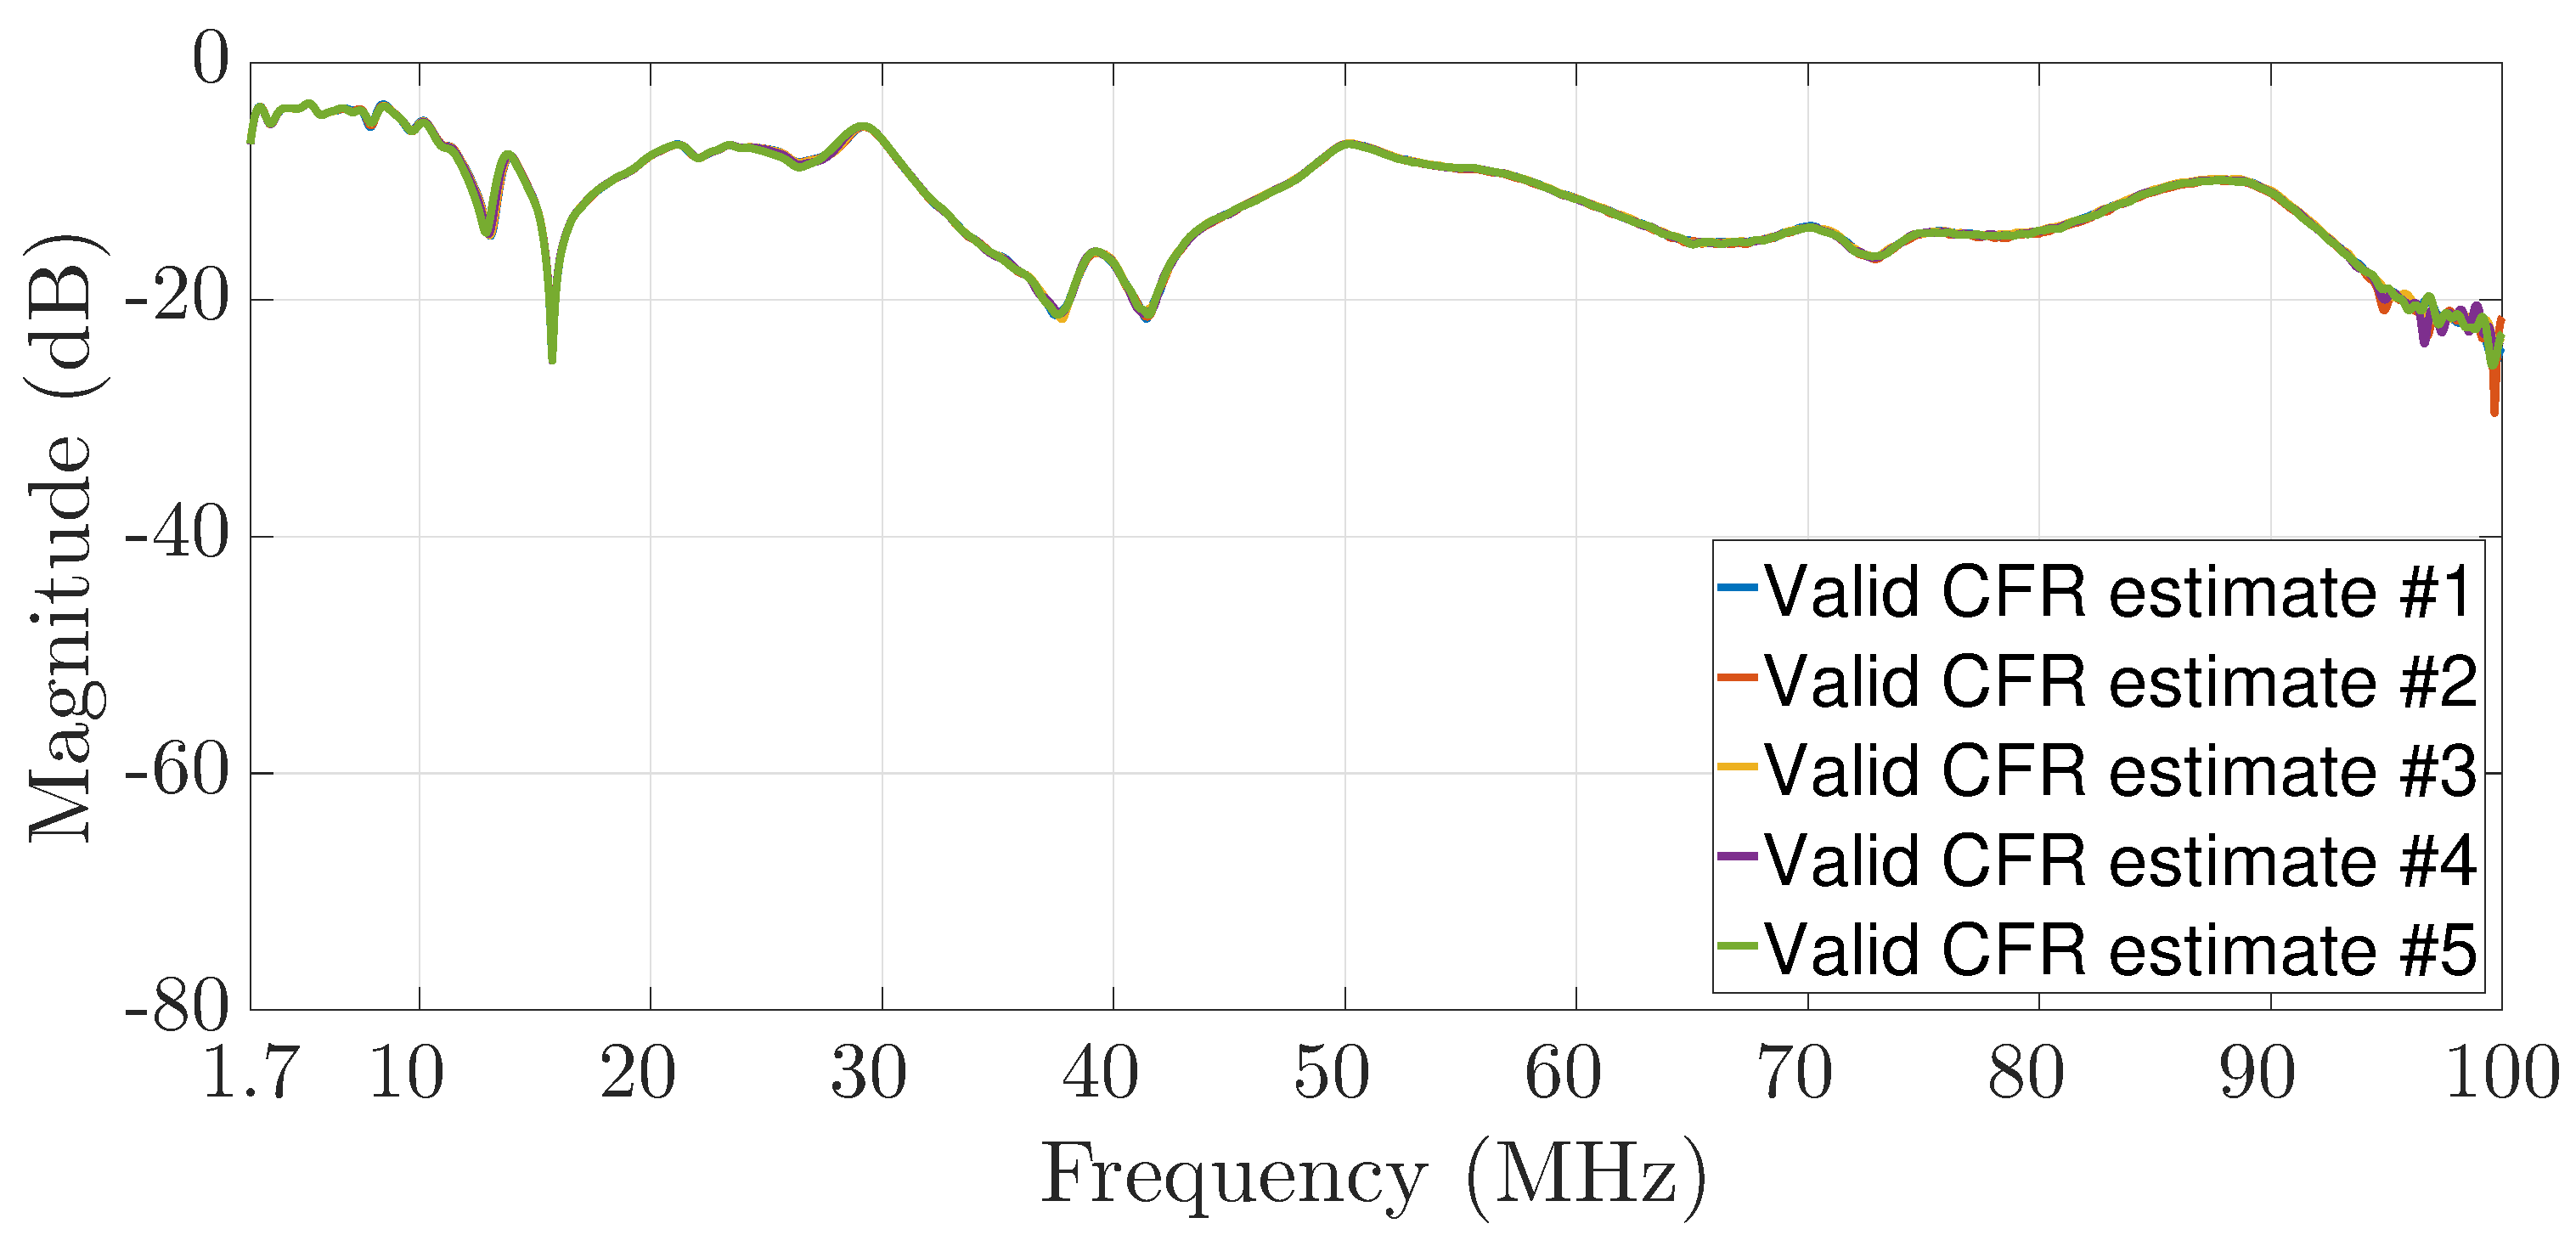
\includegraphics[width=0.9\textwidth]{images/respfreq_17.eps}
	\caption{Five consecutive and valid CFR Magnitudes of the measured in-home PLC channel.}
	\label{respfreq}
\end{figure}

Fig. \ref{MAG_percent} illustrates the relative frequency of statistical distributions that had modeled, in accordance with the adopted criteria, the magnitude of the whole data set of valid \ac{CFR} estimates. It is noted that there is not only a single distribution that models the majority of the magnitudes, but three different statistical distributions that stand out as possible candidates to model the \ac{CFR} magnitudes, among the chosen statistical distributions. As a matter of fact, in 35\% of the \ac{CFR} estimates data set the Beta distribution resulted in the best model, in 30\% of it the Birnbaum-Saunders distribution offered the best modeling and in 24\% of it the Log-normal distribution yielded the best modeling. 

\begin{figure}[h!]
	\centering
	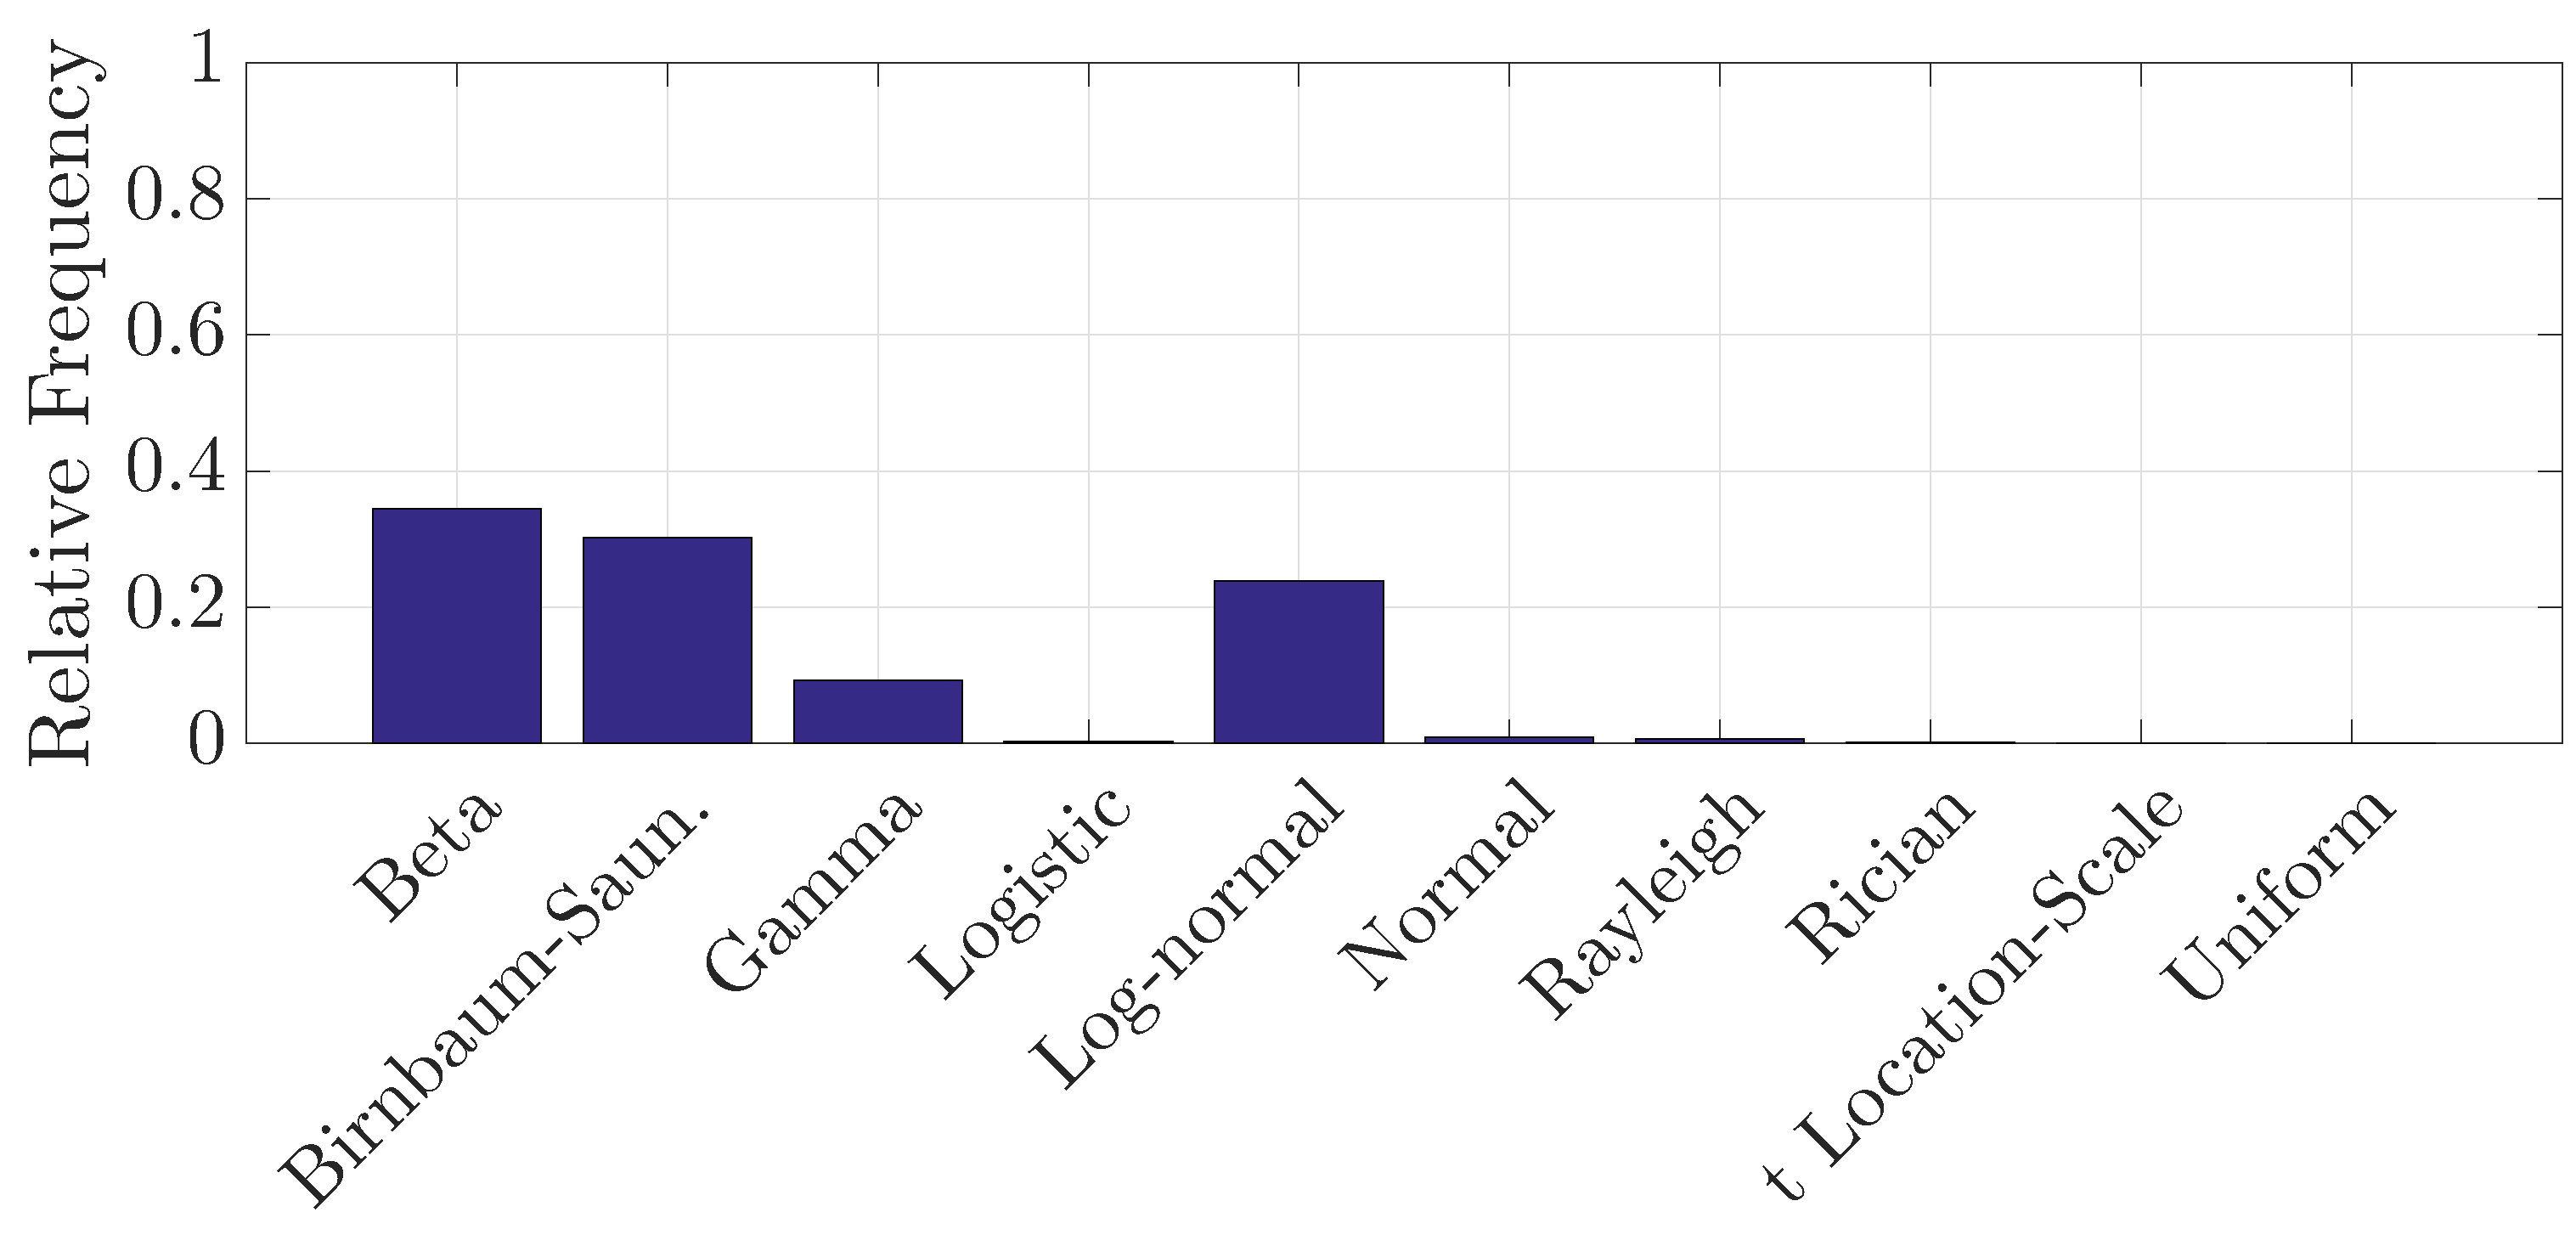
\includegraphics[width=0.9\textwidth]{images/Mag_percent.eps}
	\caption{The relative frequency associated with the chosen statistical distribution that best models the CFR magnitude in accord with the adopted criteria.}
	\label{MAG_percent}
\end{figure}

In order to evaluate which of the three statistical distributions is the best choice for modeling the magnitude of the \ac{CFR} estimates, we use the log-likelihood ratio $\rho_{MLE} (f)$ (\ref{eq:log-lik}) as defined in subsection \ref{sec:P1}, where the set of statistical distribution is denote by $\mathcal{A}\in\{${Beta, Birnbaum-Saunders, Gamma, Logistic, Log-normal, Normal, Rayleigh, Rician, t Location-Scale, Uniform}$\}$. It is important to emphasize that the choice of $\rho_{MLE} (f)$ is for illustrating the results in continuous-time domain.  Fig. \ref{fig:Log_like} shows the values of $\rho_{MLE}(f)$ for the three best statistical distributions candidates to model the magnitude of the valid \ac{CFR} estimates. The threshold value $1.2$, corresponding to a deviation of $20\%$ from the best achievable result, was heuristically chosen as the upper bound, indicated by a red dashed line, under which the statistical distribution can be considered good enough to model the \ac{CFR} of in-home \ac{PLC} channels. Note that the vertical axis was limited to the range between $0$ and $5.0$ to facilitate the visualization and the comparison among the log-likelihood ratio ($\rho_{MLE} (f)$) curves. These curves emphasize the suitability of the Beta distribution to model the samples of the magnitude of the valid \ac{CFR} estimates. Overall, the results showed in Fig. \ref{MAG_percent} and Fig. \ref{fig:Log_like} strongly suggest the use of the Beta distribution to model the magnitude of the valid \ac{CFR} estimates of the measured in-home Brazilian \ac{PLC} channels. In other words, the magnitude of the valid \ac{CFR} estimates of in-home \ac{PLC} channels can be modeled by using only one statistical distribution (i.e., the Beta distribution).

%\begin{figure}[h!]
%	\centering
%	\psfrag{AAA}[c][c][1.3]{$\rho_{MLE} (f)$}
%	\subfloat[]{\includegraphics[width=0.9\textwidth]{images/Log_Beta_17.eps}}\\~\\
%	\psfrag{AAA}[c][c][1.3]{$\rho_{MLE} (f)$}
%	\subfloat[]{\includegraphics[width=0.9\textwidth]{images/Log_Birn_17.eps}}\\~\\
%	\psfrag{AAA}[c][c][1.3]{$\rho_{MLE} (f)$}
%	\subfloat[]{\includegraphics[width=0.9\textwidth]{images/Log_LogN_17.eps}}
%	\caption{The log-likelihood ratio for the following statistical distributions: (a) Beta, (b) Birnbaun-Saunders, and (c) Log-normal.}
%	\label{fig:Log_like}
%\end{figure}

\begin{figure}[h!]
	\centering
	\psfrag{AAA}[c][c][1.3]{$\rho_{MLE} (f)$}
	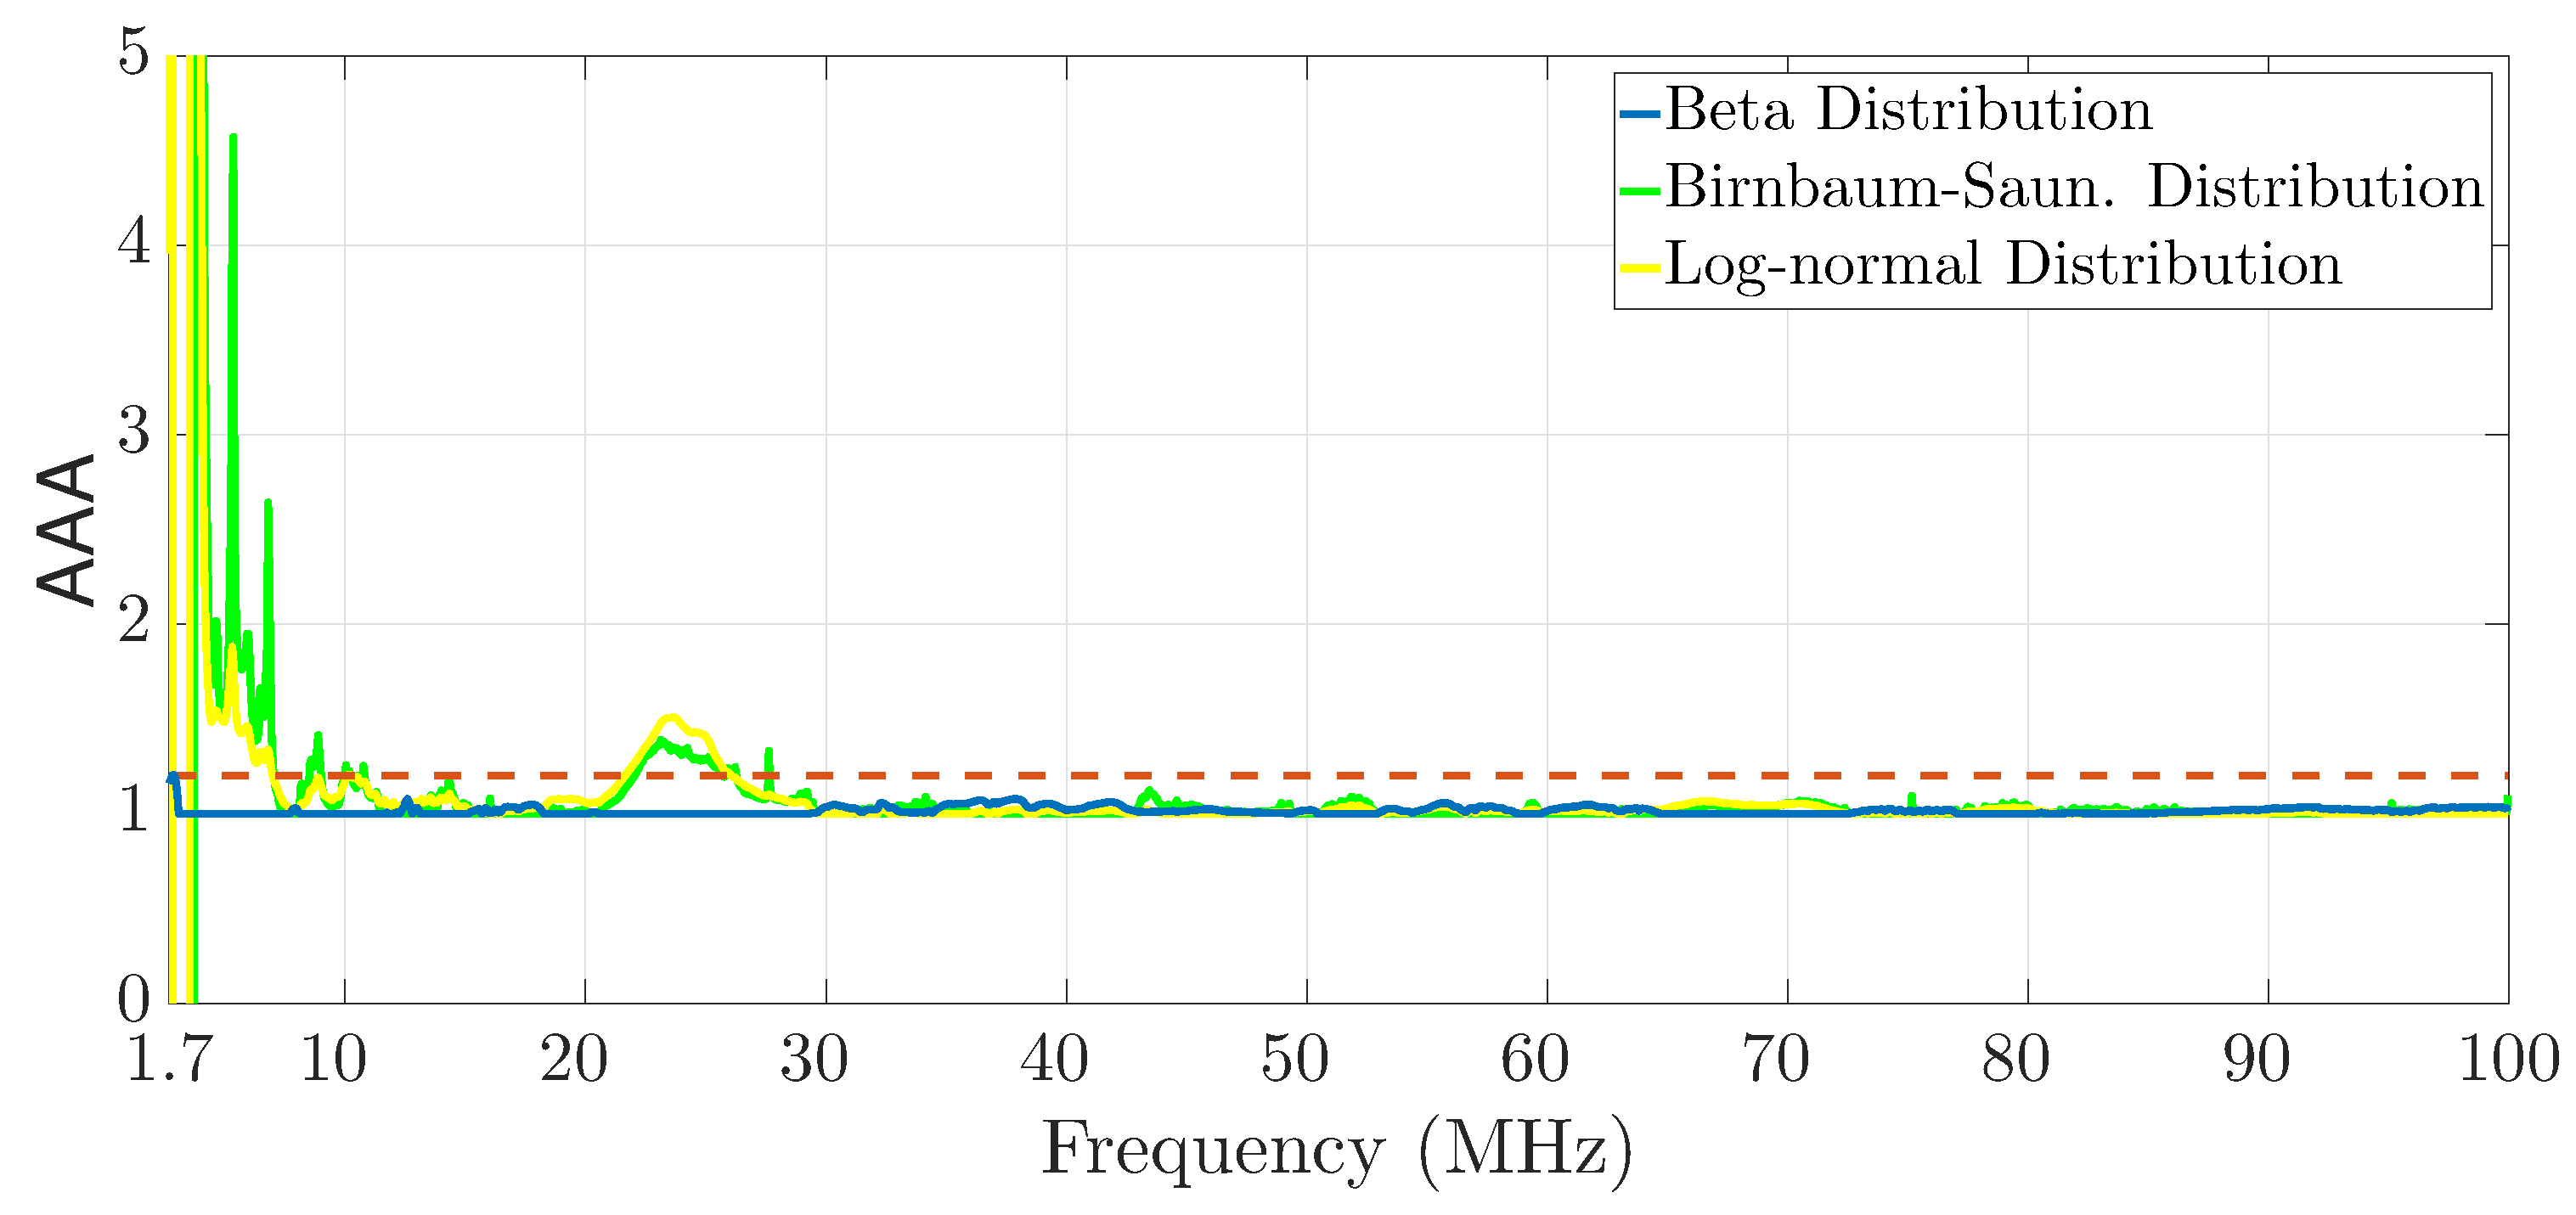
\includegraphics[width=0.9\textwidth]{images/LLH_BETA_BIRN_LogN_1.7.eps}
	\caption{The log-likelihood ratio for the following statistical distributions: Beta, Birnbaun-Saunders, and Log-normal.}
	\label{fig:Log_like}
\end{figure}

The statistical analysis of the magnitude of the valid \ac{CFR} estimates shows that the parameters of the Beta distribution assume different values as frequency changes. If $\mathcal{C}_{k} = \{\zeta_{1}[k],\zeta_{2}[k]\}$ is the set of parameters for the statistical distribution modeling the magnitude of the valid \ac{CFR} estimates of in-home \ac{PLC} channels, where $k=0,1,\cdots,N-1$, $\zeta_{1}[k] = \alpha[k]$ and $\zeta_{2}[k] = \beta[k]$, are the two shape parameters ($U=2$) of the Beta distribution associated with the $k$-th sample of the valid \ac{CFR} in the discrete-time domain. Then, Fig. \ref{mag_example} and Fig. \ref{mag_example2} portrays the statistical models for two different values of frequency: $f=52.1$~MHz ($k=1067 \rightarrow f= 1067\Delta f$) and $f=78.1$~MHz ($k=1600 \rightarrow f = 1600\Delta f$), respectively. The parameters of the Beta distribution are $\alpha(1067 \Delta f) = \zeta_{1}[1067]=0.717$ and $\beta( 1067 \Delta f) = \zeta_{2}[1067] = 10.435$; $\alpha(1600 \Delta f) = \zeta_{1}[1600] = 0.780$ and $\beta( 1600 \Delta f) = \zeta_{2}[1600]=17.772$ for $f=52.1$~MHz and $f=78.1$~MHz, respectively.

\begin{figure}[h!]
	\centering
	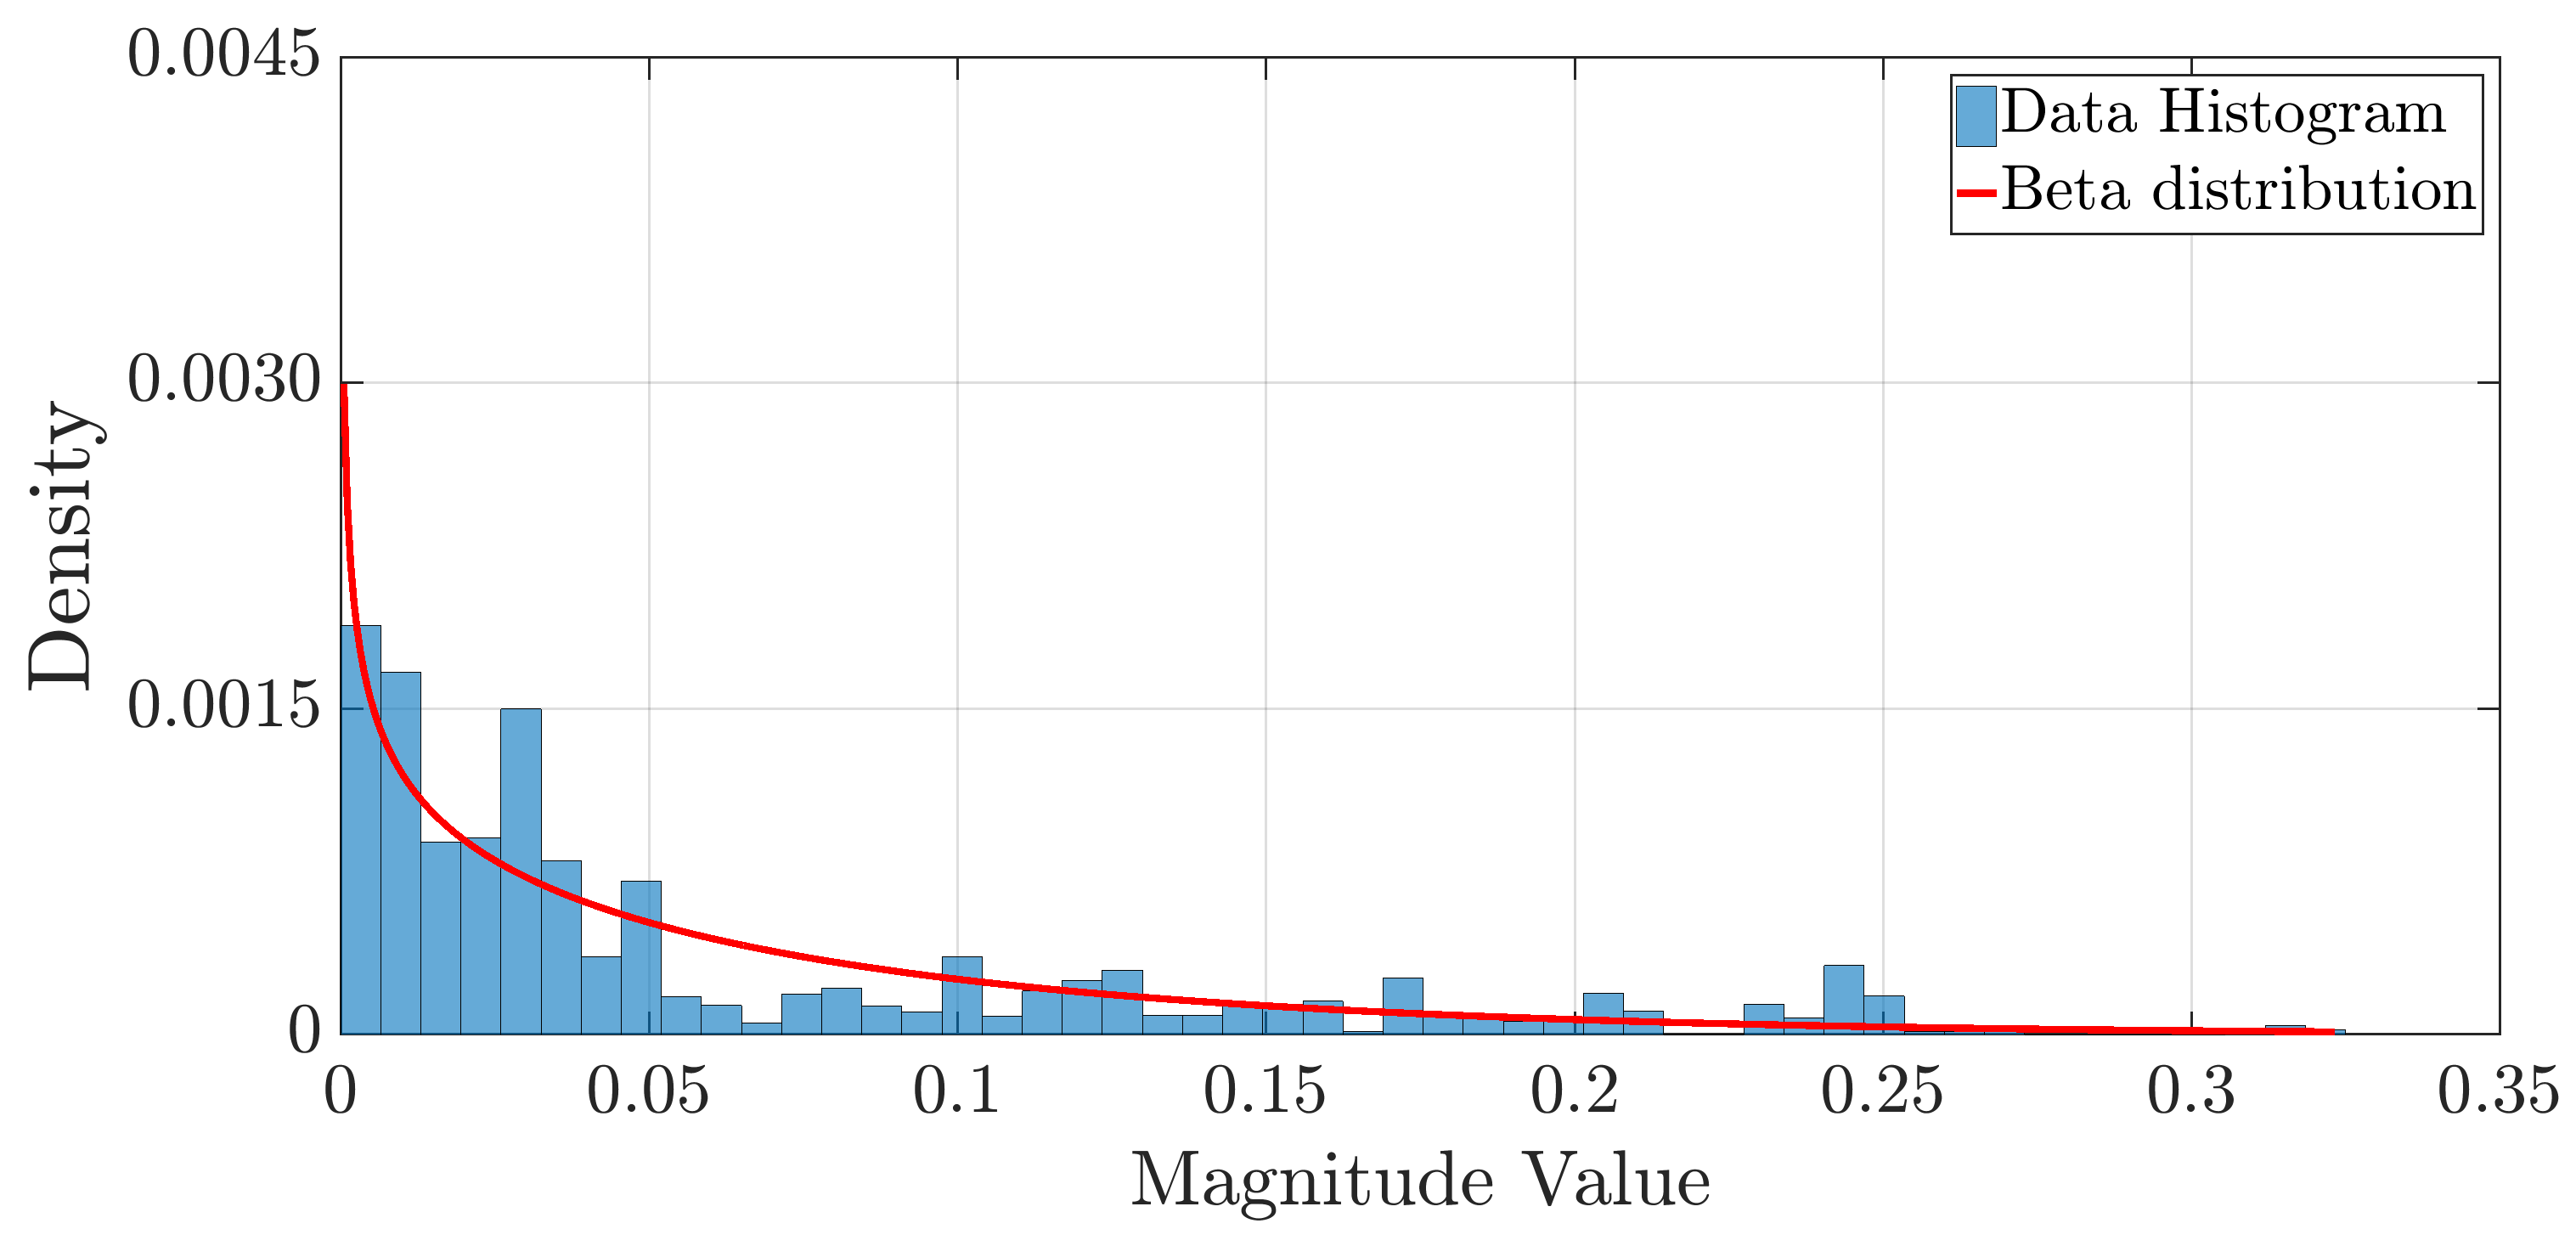
\includegraphics[width=0.9\textwidth]{images/Mag_hist_2.eps}
	\caption{The relative frequency of the magnitude of the valid CFR estimates at the sample $k = 1067$ ($k\Delta f= 52.1$~MHz) and the modeling based on the Beta distribution.}
	\label{mag_example}
\end{figure}

\begin{figure}[h!]
	\centering
	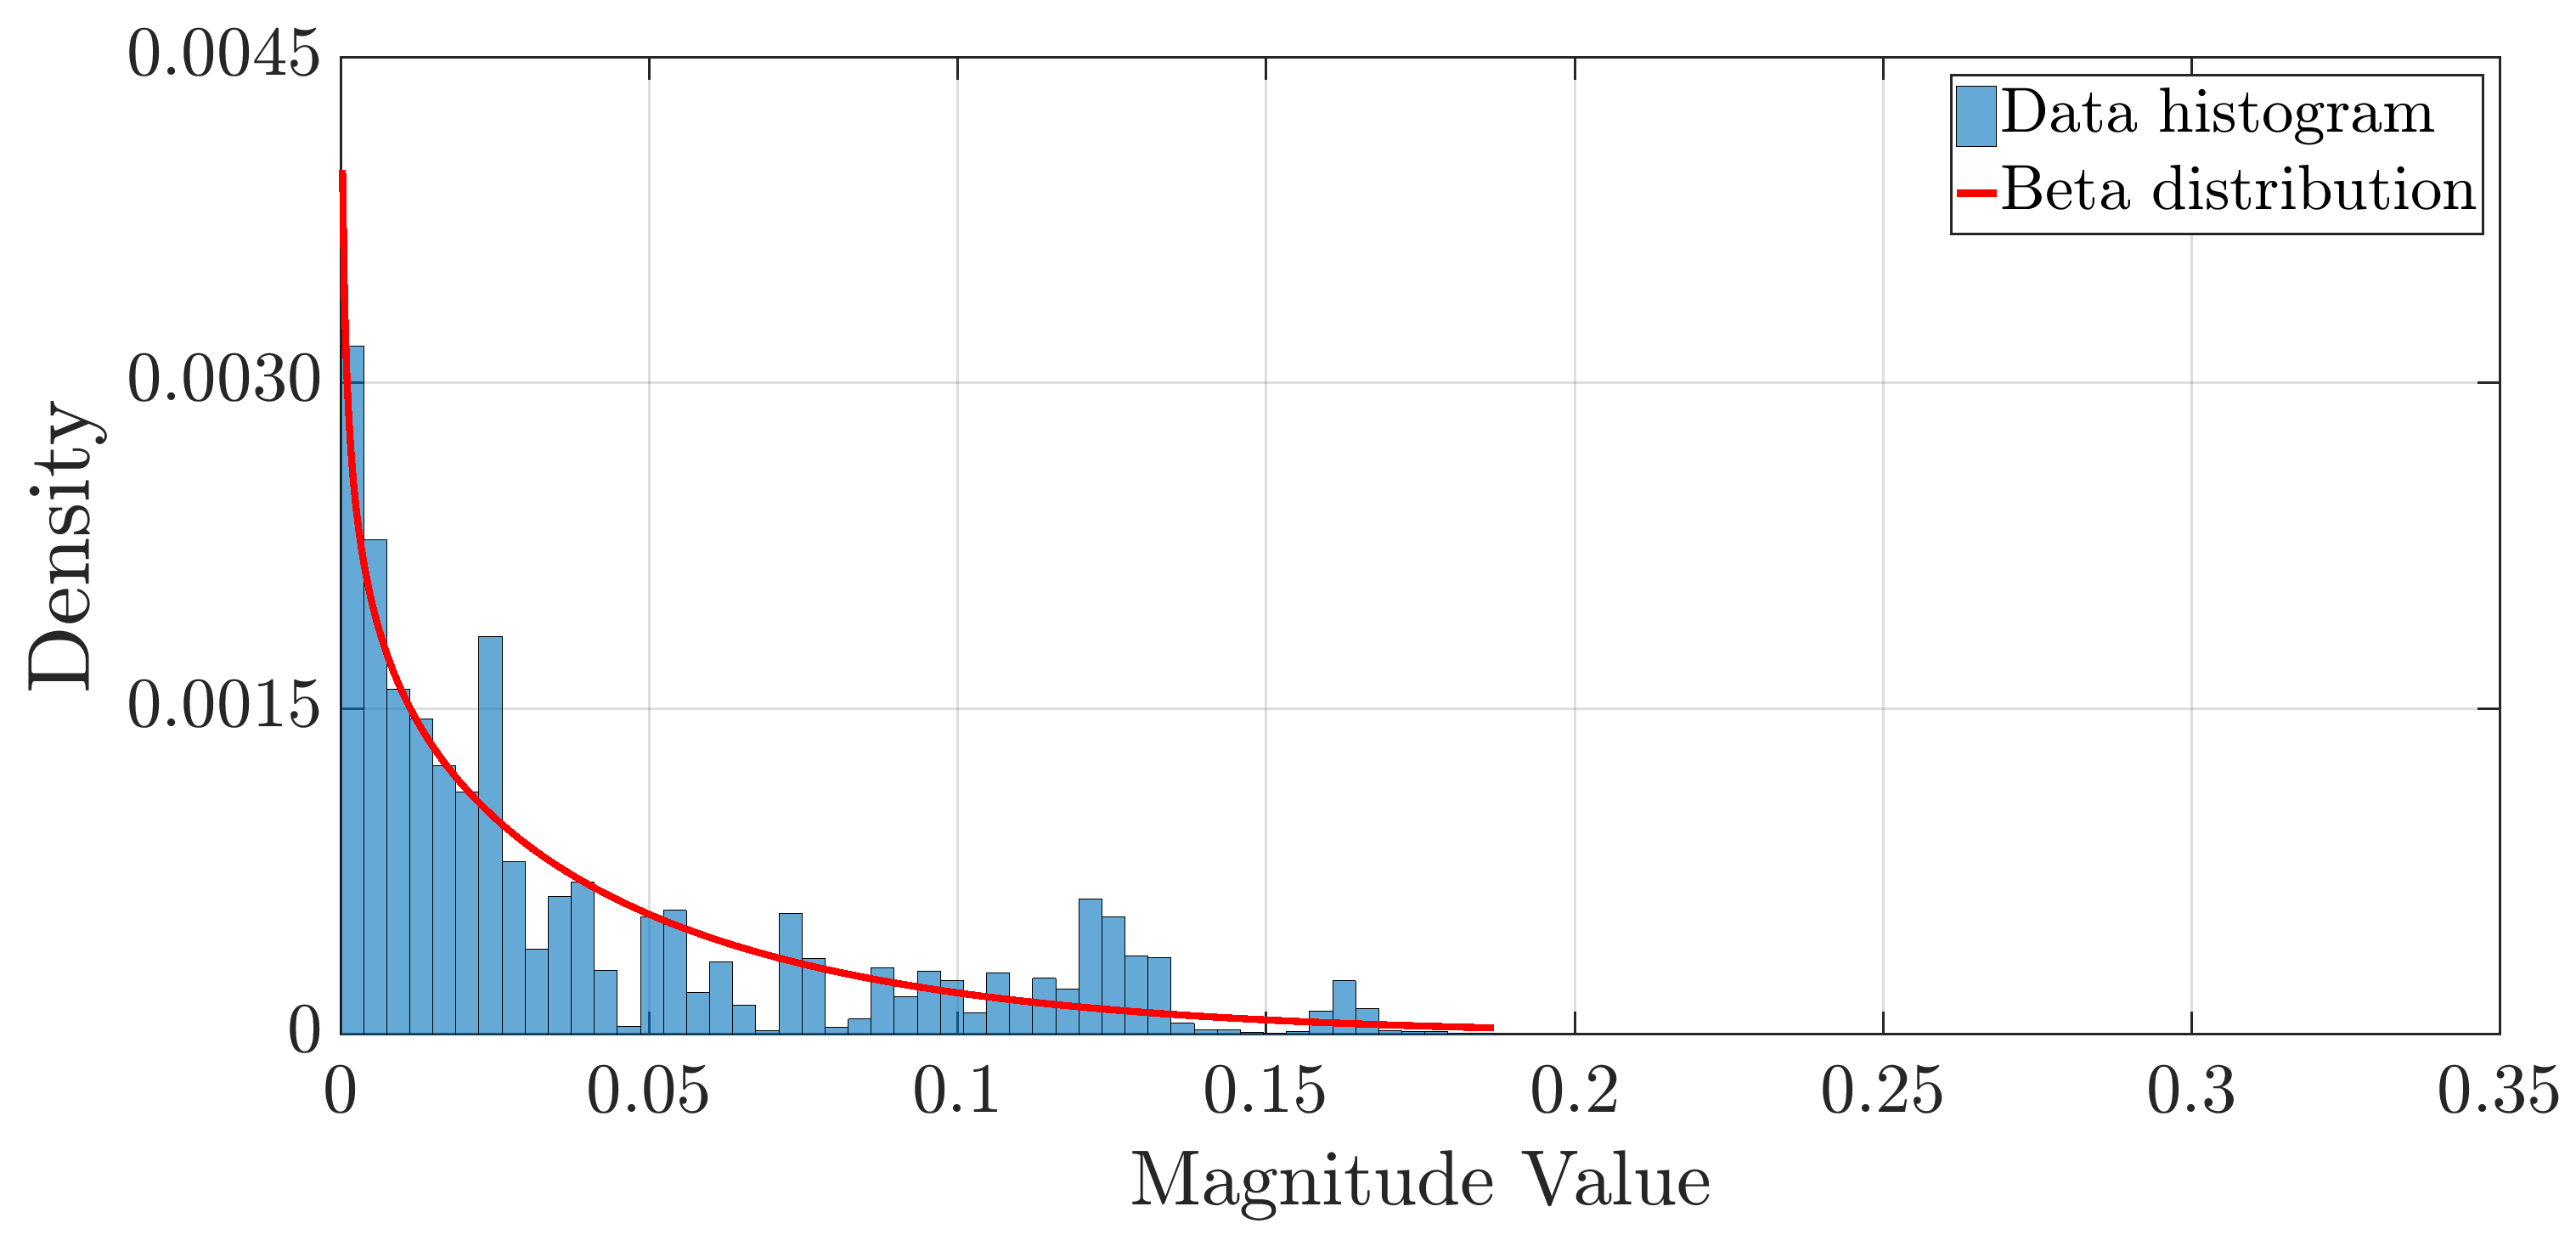
\includegraphics[width=0.9\textwidth]{images/Mag_hist2_2.eps}
	\caption{ The relative frequency of the magnitude of the valid CFR estimates at the sample $k = 1600$ ($k\Delta f= 78.1$~MHz) and the modeling based on the Beta distribution.}
	\label{mag_example2}
\end{figure}

Fig. \ref{fig:boundsPLC} illustrates the \ac{MSE} results in terms of the number of subbands for the in-home \ac{PLC} channels. According to this plot, independent of the chosen criterion to select the non-uniformity of the subbands, the \ac{MSE} value does not change significantly as the number of subbands becomes higher than $19$. Due to a trade off between the precision of the interpolation and complexity of the computation, $L=19$ was chosen as the number of subbands. By interpolating the parameters values $\alpha[k]$ and $\beta[k]$ of the Beta distributions using $L=19$ subbands and the Algorithm \ref{Algo2}, the continuous curves of parameters $\hat{\alpha}(\omega)$ and $\hat{\beta}(\omega)$ are yielded. Finally, the curves $\hat{\alpha}(f)$ and $\hat{\beta}(f)$ are easily obtained because $\omega \in [0,\pi)$ directly corresponds to the frequency band between $0$ and $100$~MHz. Figs. \ref{Fit_alfa} and \ref{Fit_beta} illustrates the curves for the parameters $\alpha(f)$ and $\beta(f)$, which are obtained by applying frequency domain interpolation technique detailed in \cite{mitra} and the curves obtained by using the cubic Spline interpolation with $L=19$ subbands. For the sake of comparison Fig. \ref{Fit_alfa_poli} shows the curves for parameter $\alpha(f)$ obtained, by applying the frequency domain interpolation technique detailed in \cite{mitra} and by using the interpolation technique discussed in \cite{Luis:AI} applied over $L=19$ subbands denoted by $20$ equally spaced interval bounds, over the desired frequency bandwidth. On this figure is possible to notice the presence of edge effects that occurs in the boundaries between two polynomials, which are interpolating the values of the parameters in two consecutive frequency subbands. Note that Table \ref{table_alfa}, in Appendix \ref{ap:c}, lists the cubic Spline coefficients for modeling the parameter $\alpha(f)$ of the valid \ac{CFR} magnitude while Table \ref{table_beta}, also in  Appendix \ref{ap:c}, lists the cubic Spline coefficients for modeling the parameter $\beta(f)$. As a result, the Beta distribution and its coefficients waveform  $\hat{\alpha}(f)$ and $\hat{\beta}(f)$ define the random process representing the magnitude of the \ac{CFR} of the in-home \ac{PLC} channel.
  
\begin{figure}[h!]
	\centering
	\subfloat[]{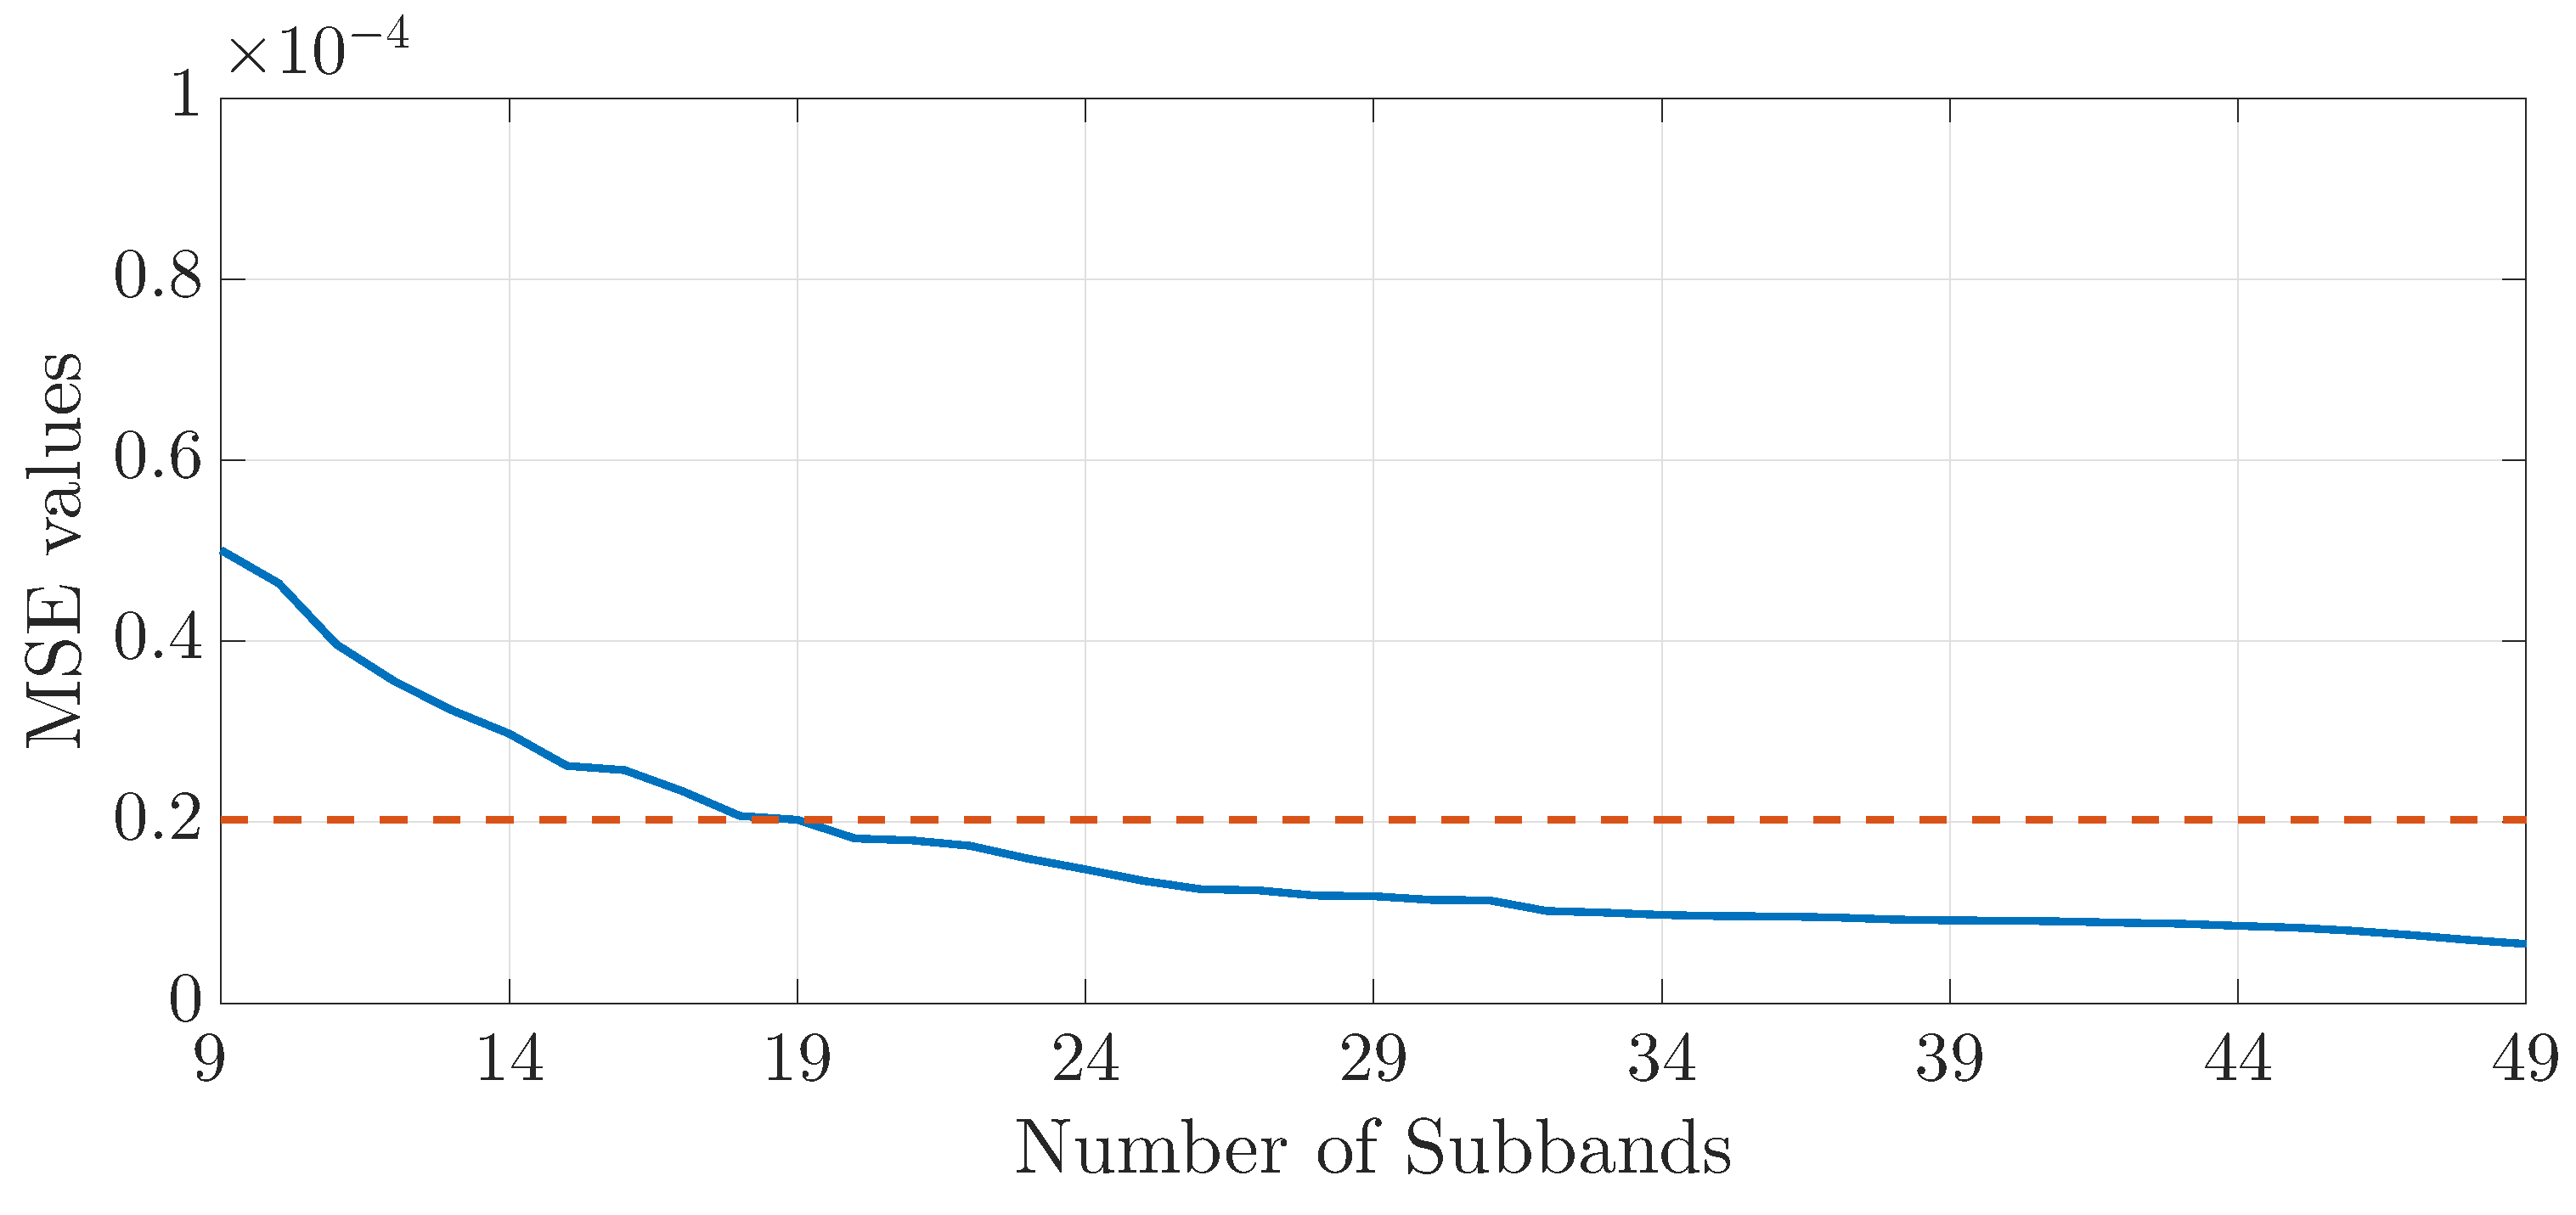
\includegraphics[width=0.9\textwidth]{images/alfa_bounds.eps}}\\~\\
	\subfloat[]{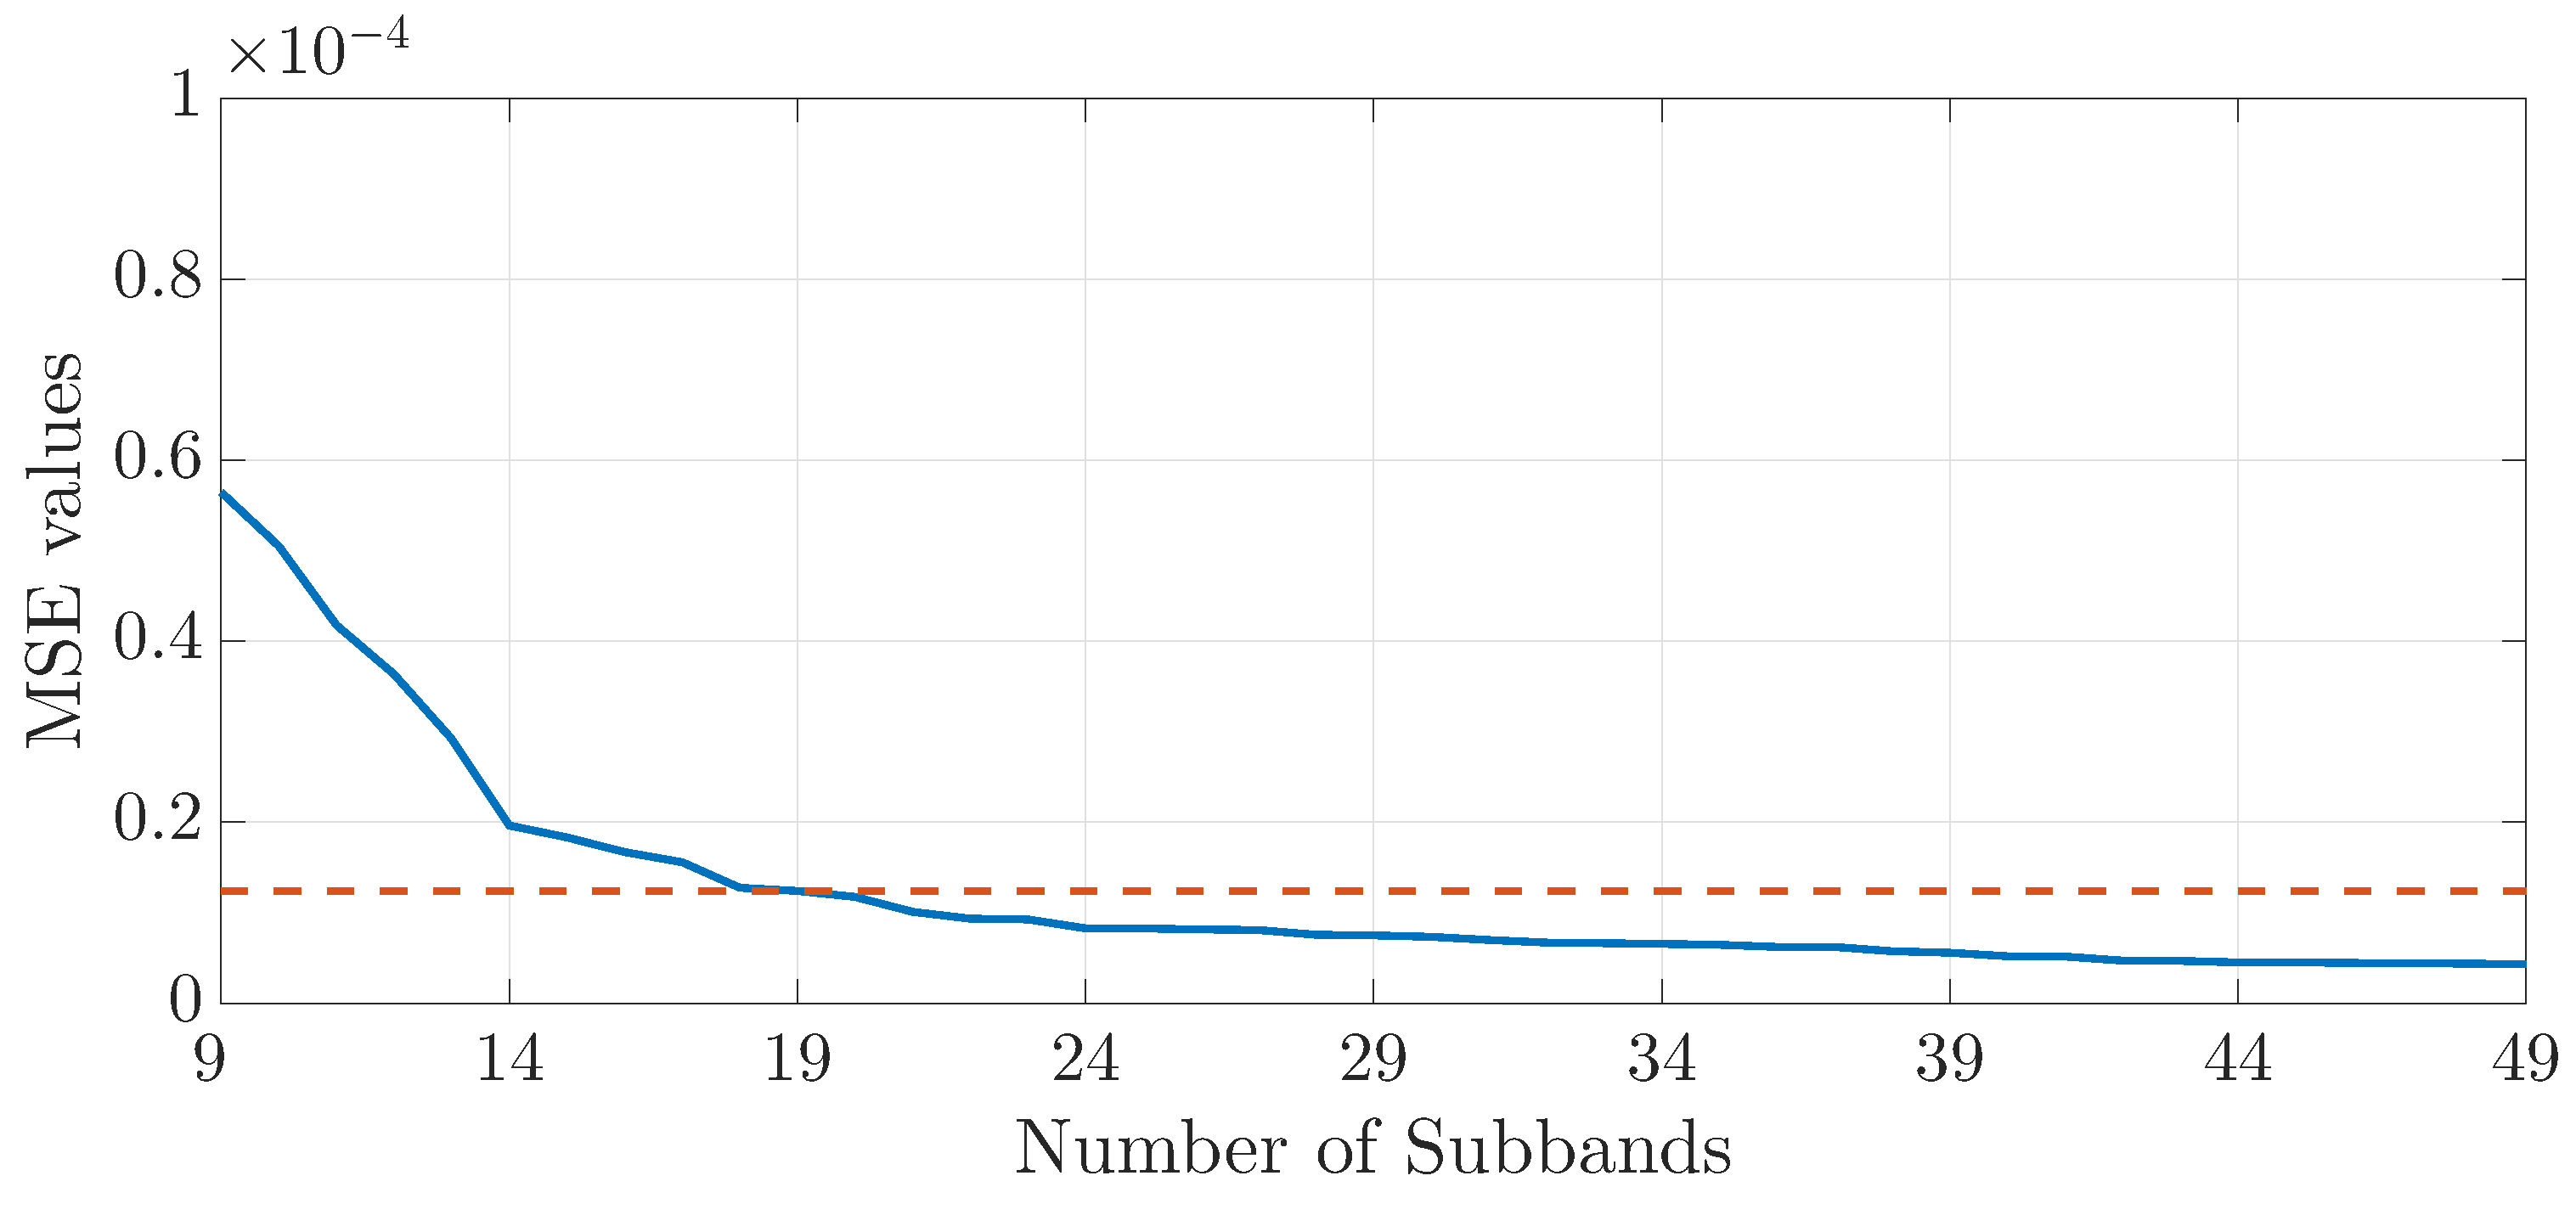
\includegraphics[width=0.9\textwidth]{images/beta_bounds.eps}}\\~\\
	\caption{The MSE values for the parameters from PLC scenario: (a) $\alpha$ parameter, (b) $\beta$ parameter.}
	\label{fig:boundsPLC}
\end{figure}
  
\begin{figure}[h]
	\centering
	\psfrag{Interval Boundsaa}[c][c][1]{Interval Bounds}
	\psfrag{AAA}[c][c][1]{$~~~~~{\alpha}(k \Delta f)$}
	\psfrag{BBB}[c][c][1]{$~\hat{\alpha}(f)$}
	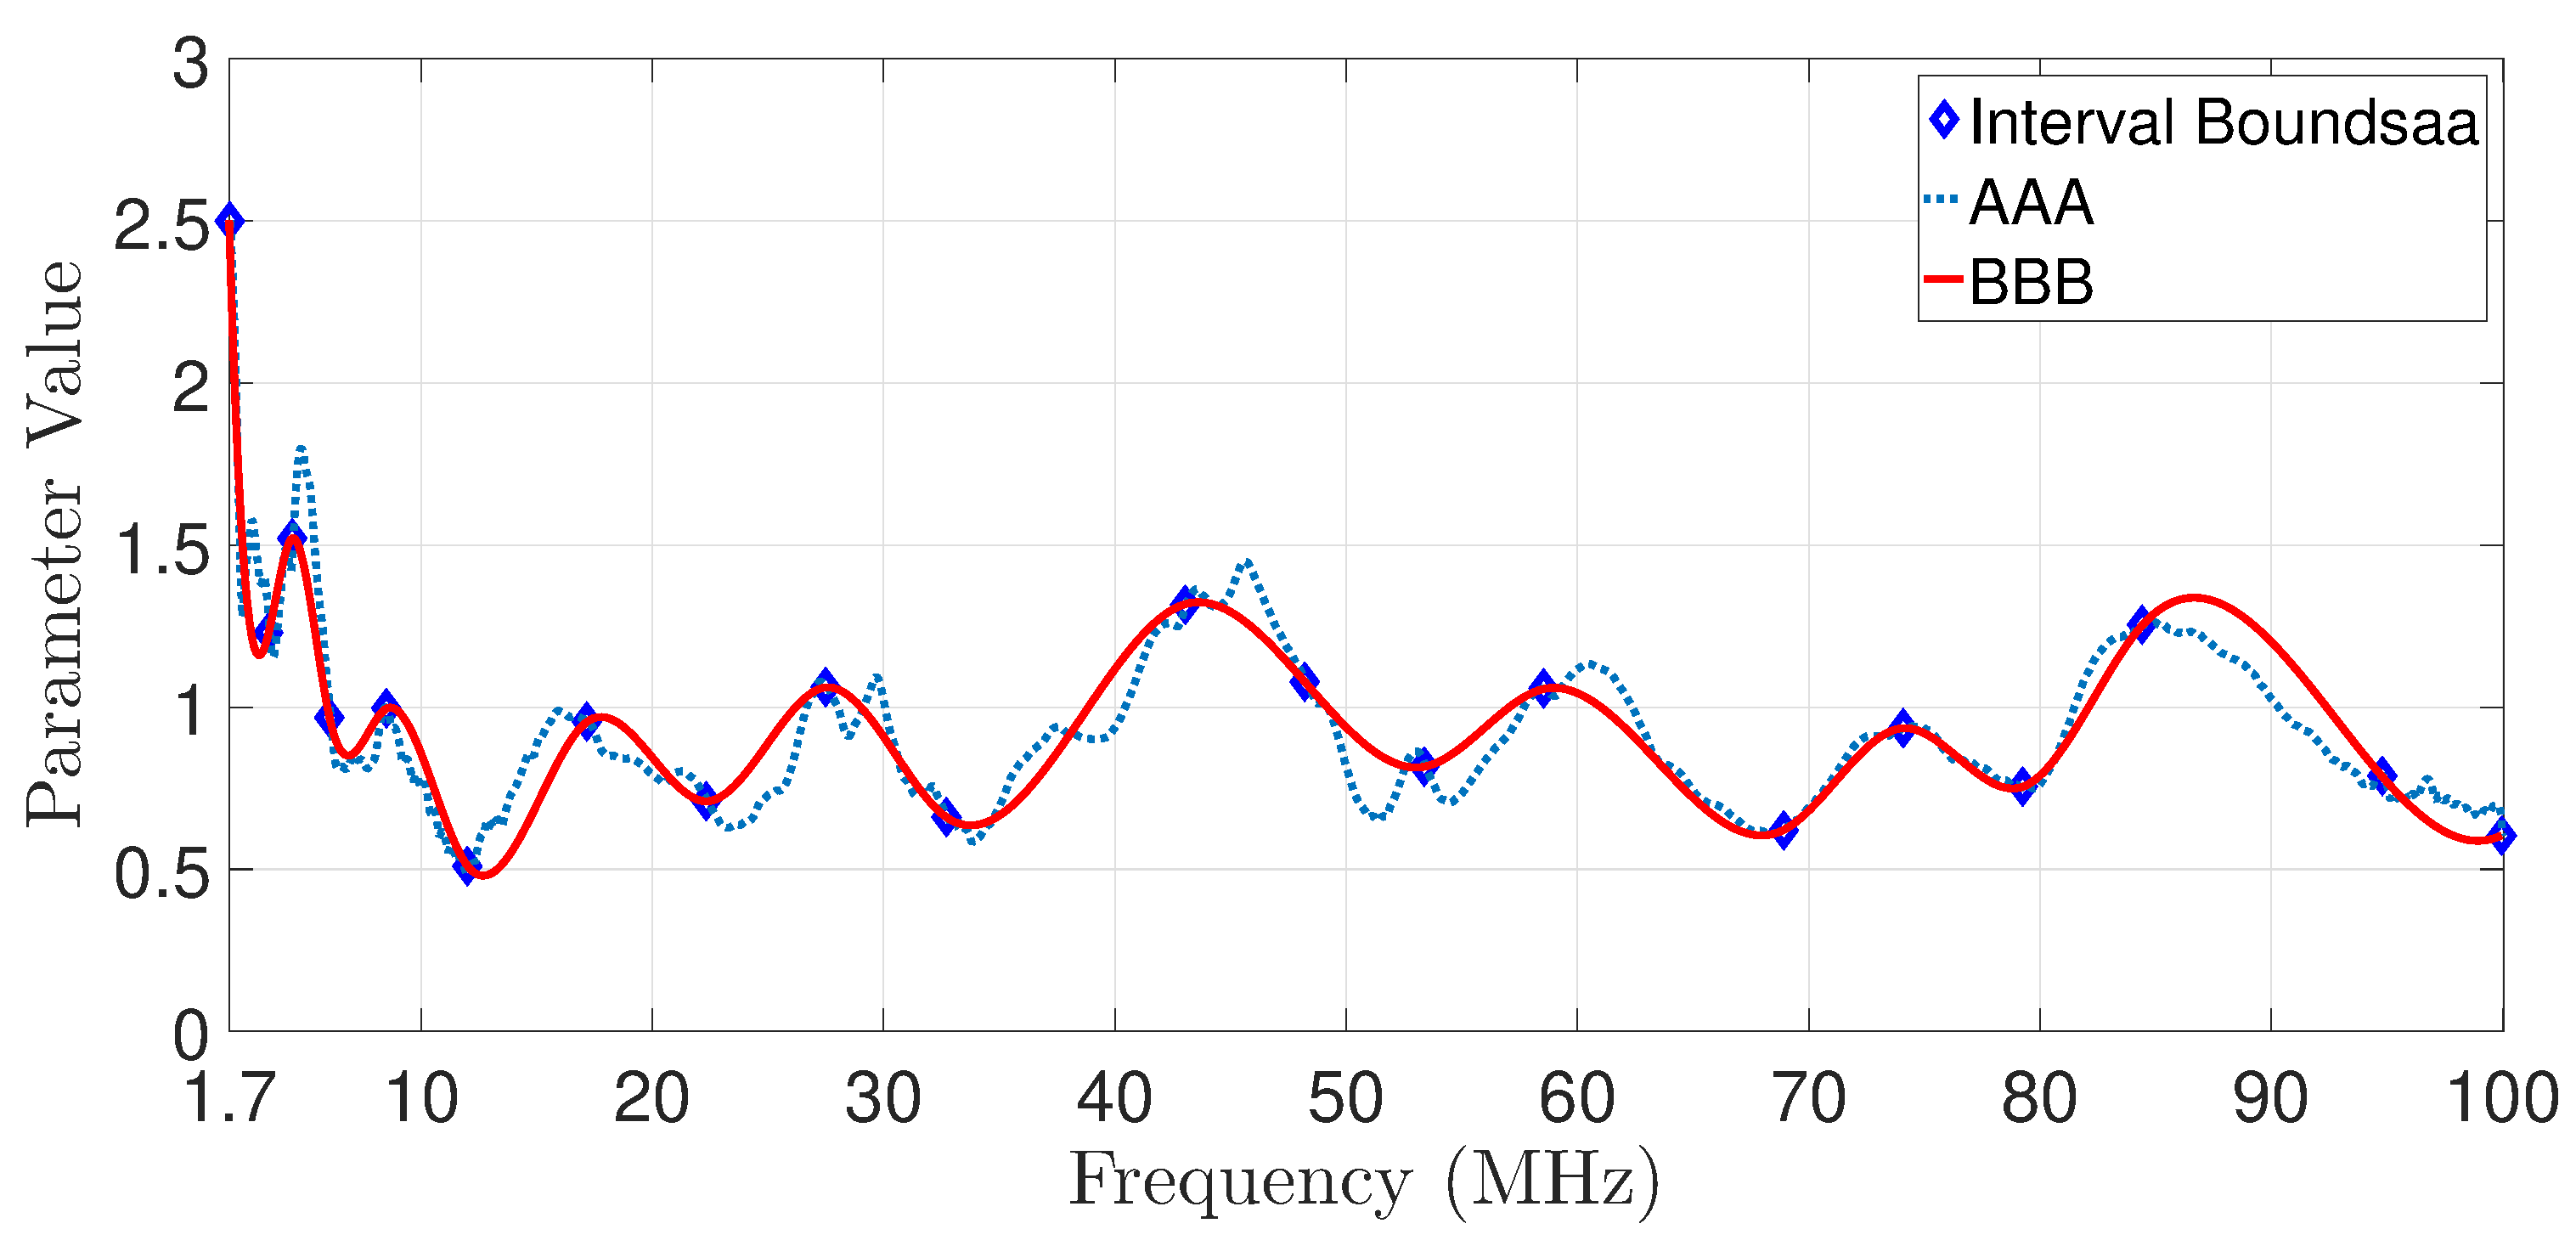
\includegraphics[width=0.9\textwidth]{images/Alfa_fit_17.eps}
	\caption{The result of the interpolation technique based on cubic Splines applied to obtain $\alpha(f)=\zeta_1(f)$ for the Beta distribution (${\alpha}(k \Delta f)$ are the original values of the parameter and $\hat{\alpha}(f)$ is the interpolated curve).}
	\label{Fit_alfa}
\end{figure}

\begin{figure}[h]
	\centering
	\psfrag{Interval Subbandsaa}[c][c][1]{Interval Bounds$~~~$}
	\psfrag{AAA}[c][c][1]{$~~~~~{\alpha}(k \Delta f)$}
	\psfrag{BBB}[c][c][1]{$~~~~~~~~~~~~~~~l^{th}$ Polynomial}
	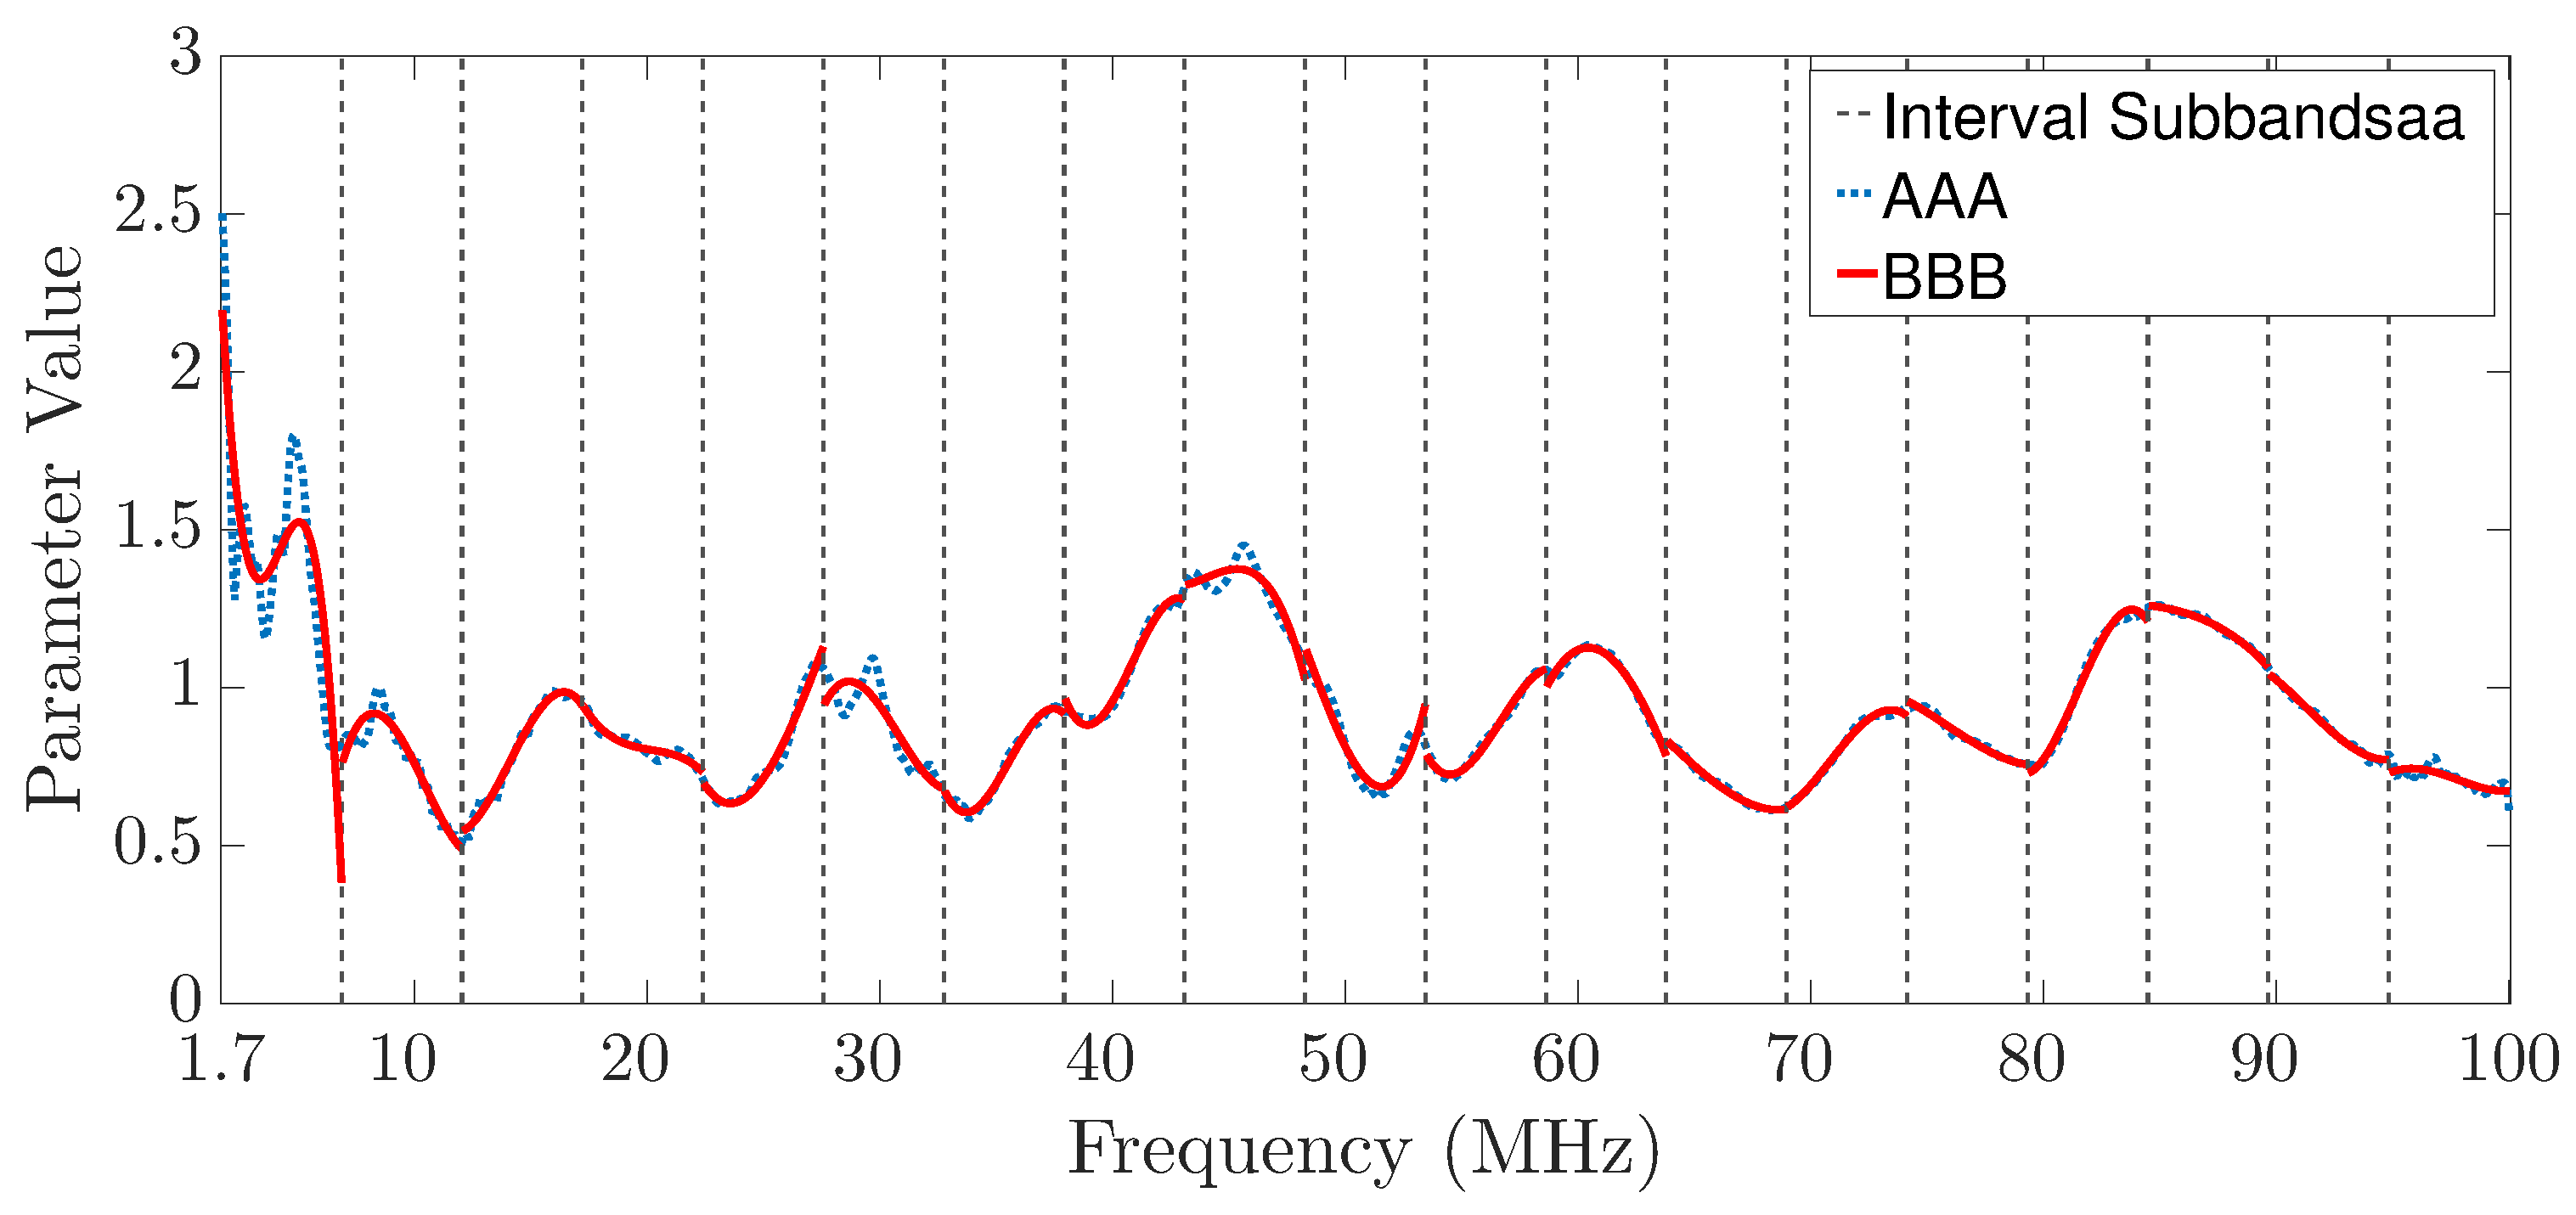
\includegraphics[width=0.9\textwidth]{images/SPLINE_Polynomials.eps}
	\caption{The result of the interpolation technique based on cubic Splines applied to obtain $\alpha(f)=\zeta_1(f)$ for the Beta distribution (${\alpha}(k \Delta f)$ are the original values of the parameter and $\hat{\alpha}(f)$ is the interpolated curve).}
	\label{Fit_alfa_poli}
\end{figure}

\begin{figure}[h]
	\centering
	\psfrag{Interval Boundsaa}[c][c][1]{Interval Bounds}
	\psfrag{AAA}[c][c][1]{$~~~~~{\beta}(k \Delta f)$}
	\psfrag{BBB}[c][c][1]{$~\hat{\beta}(f)$}
	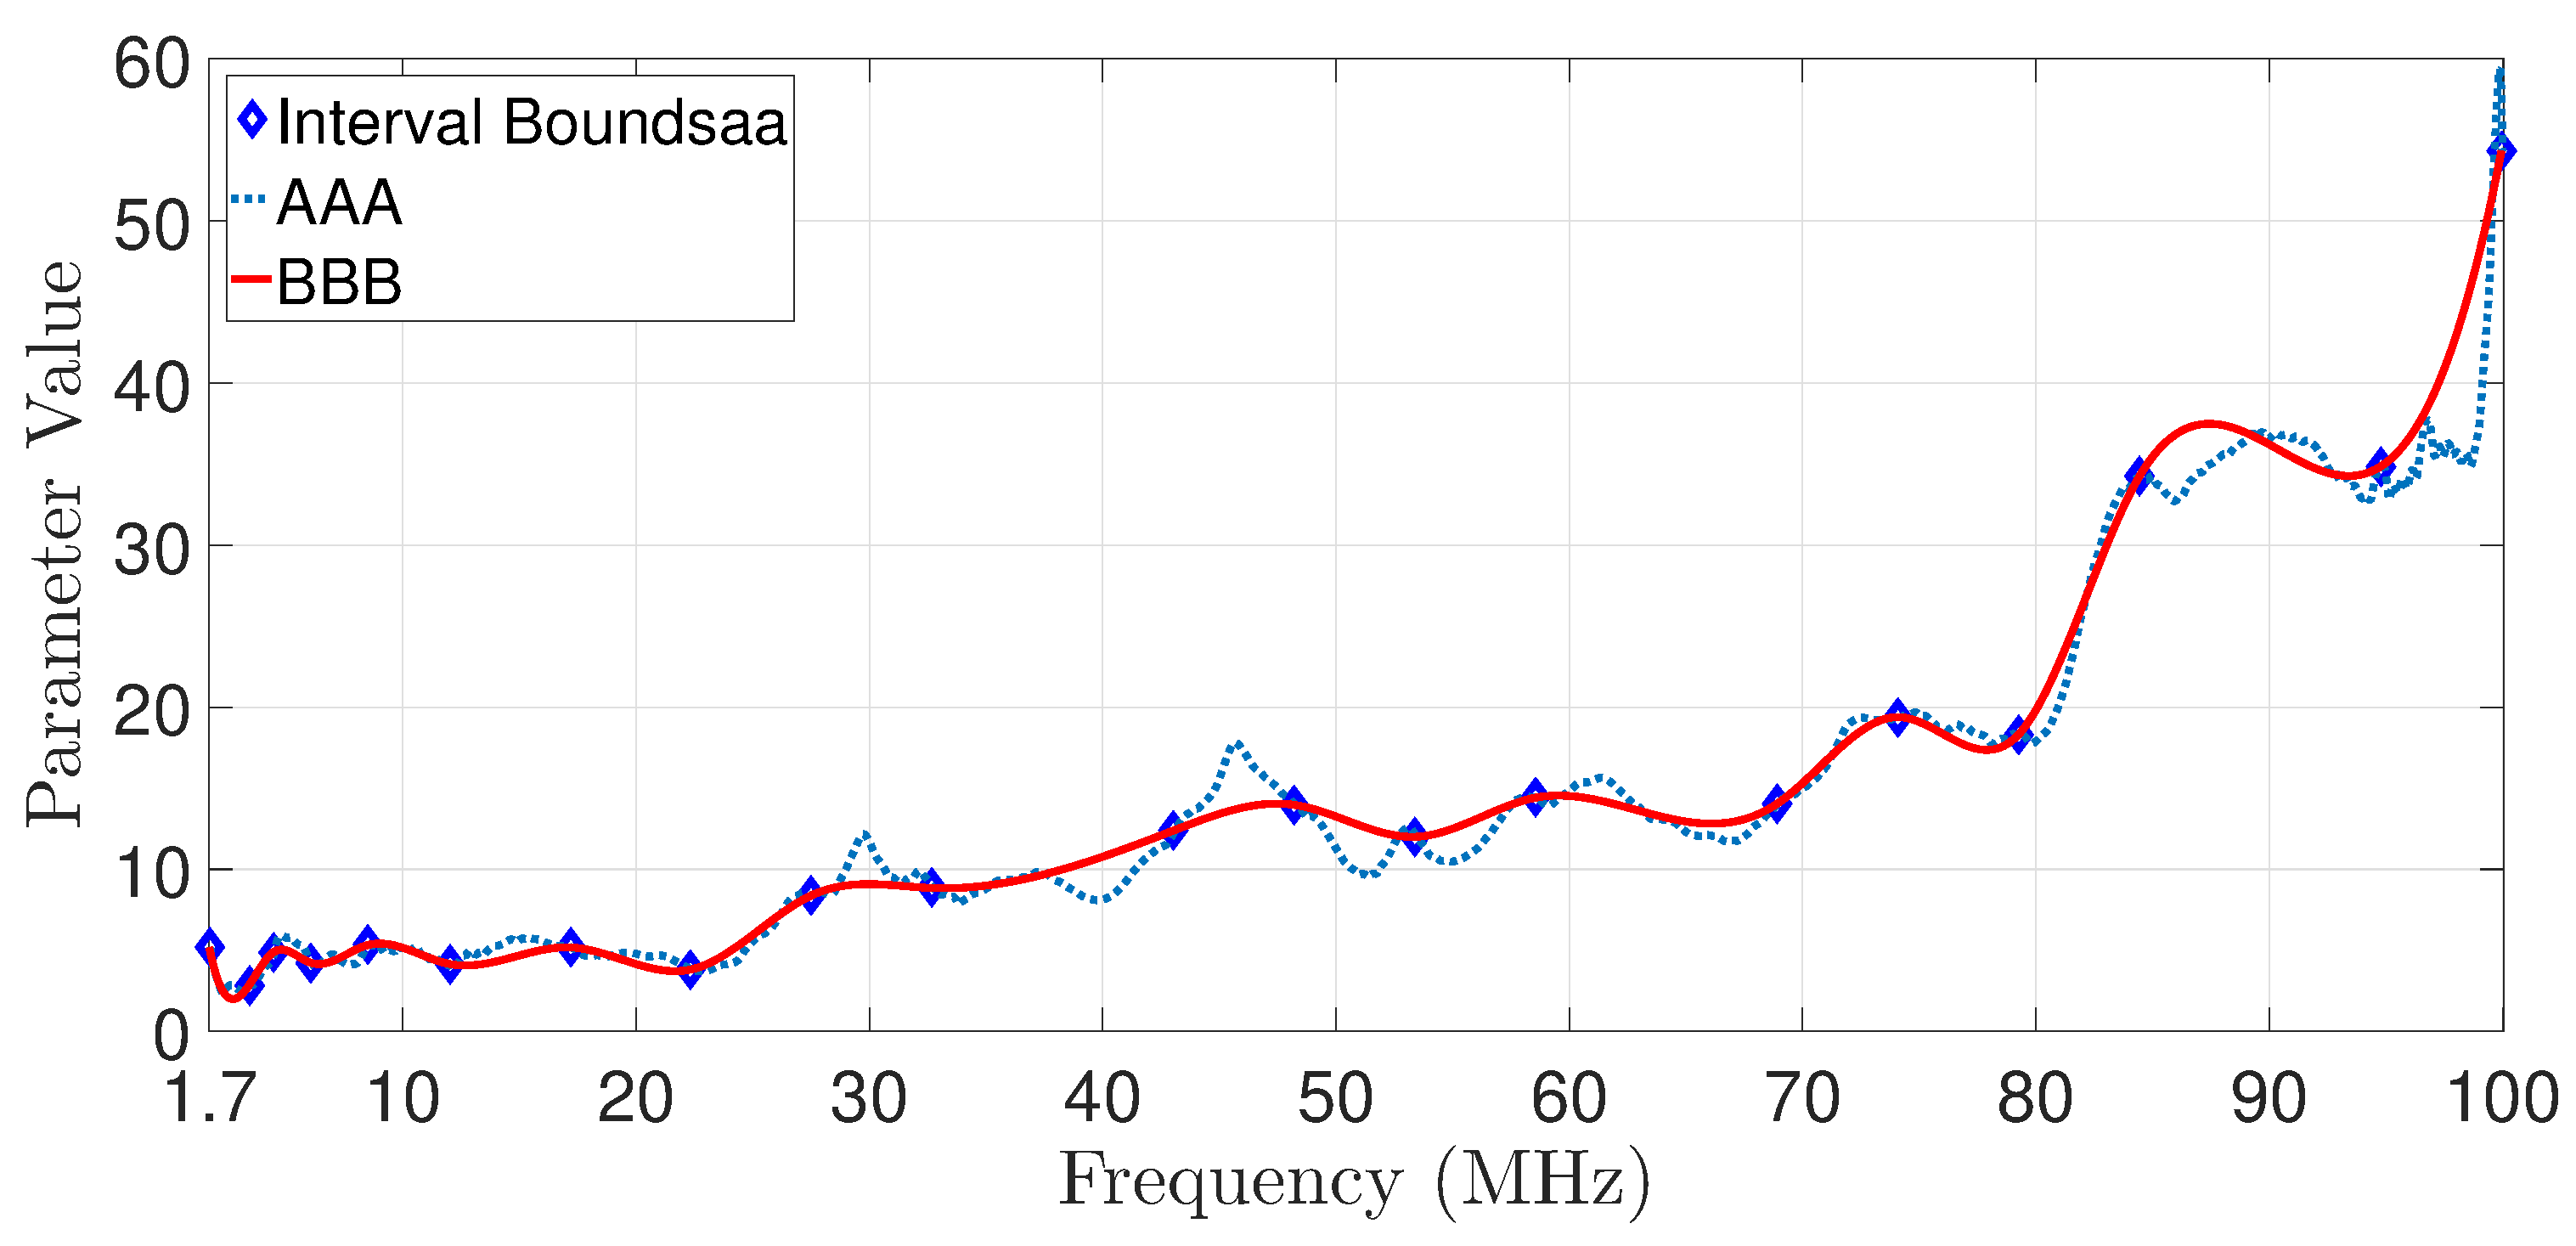
\includegraphics[width=0.9\textwidth]{images/Beta_fit_17.eps}
	\caption{The result of the interpolation technique based on cubic Splines applied to obtain $\beta(f)=\zeta_2(f)$ for the Beta distribution (${\beta}(k \Delta f)$ are the original values of the parameter and $\hat{\beta}(f)$ is the interpolated curve).}
	\label{Fit_beta}
\end{figure}

Fig. \ref{Phase_percent} portrays the relative frequency of statistical distributions that had modeled, in accordance with the adopted criteria, the phase of the whole set of valid \ac{CFR} estimates. Note that 100\% of the data set is best modeled by the Uniform distribution. On this scenario, differently from the statistical modeling of the \ac{CFR} magnitude, the statistical modeling of the phase of the valid \ac{CFR} estimates illustrates that each sample of it can be modeled by the same set of parameters of the Uniform distribution. In other words, $\Theta_k \in [0, 2\pi]$ denotes the interval of values that the phase of the valid \ac{CFR} estimates can assume and it defines the support for the Uniform distribution. 

Fig. \ref{phase_example} and Fig. \ref{phase_example2} portrays the statistical models regarding the frequencies $f=52.1$~MHz ($k=1067 \rightarrow f = 1067\Delta f$) and $f=78.1$~MHz ($k=1600 \rightarrow f = 1600\Delta f$), respectively. Independent of the frequency values, the phase model of the valid \ac{CFR} estimates remains the same. As a result, by using the Uniform distribution defined in the interval $[0, 2\pi]$, the random process representing the phase of the \ac{CFR} of the in-home \ac{PLC} channel is yielded.

\begin{figure}[h!]
	\centering
	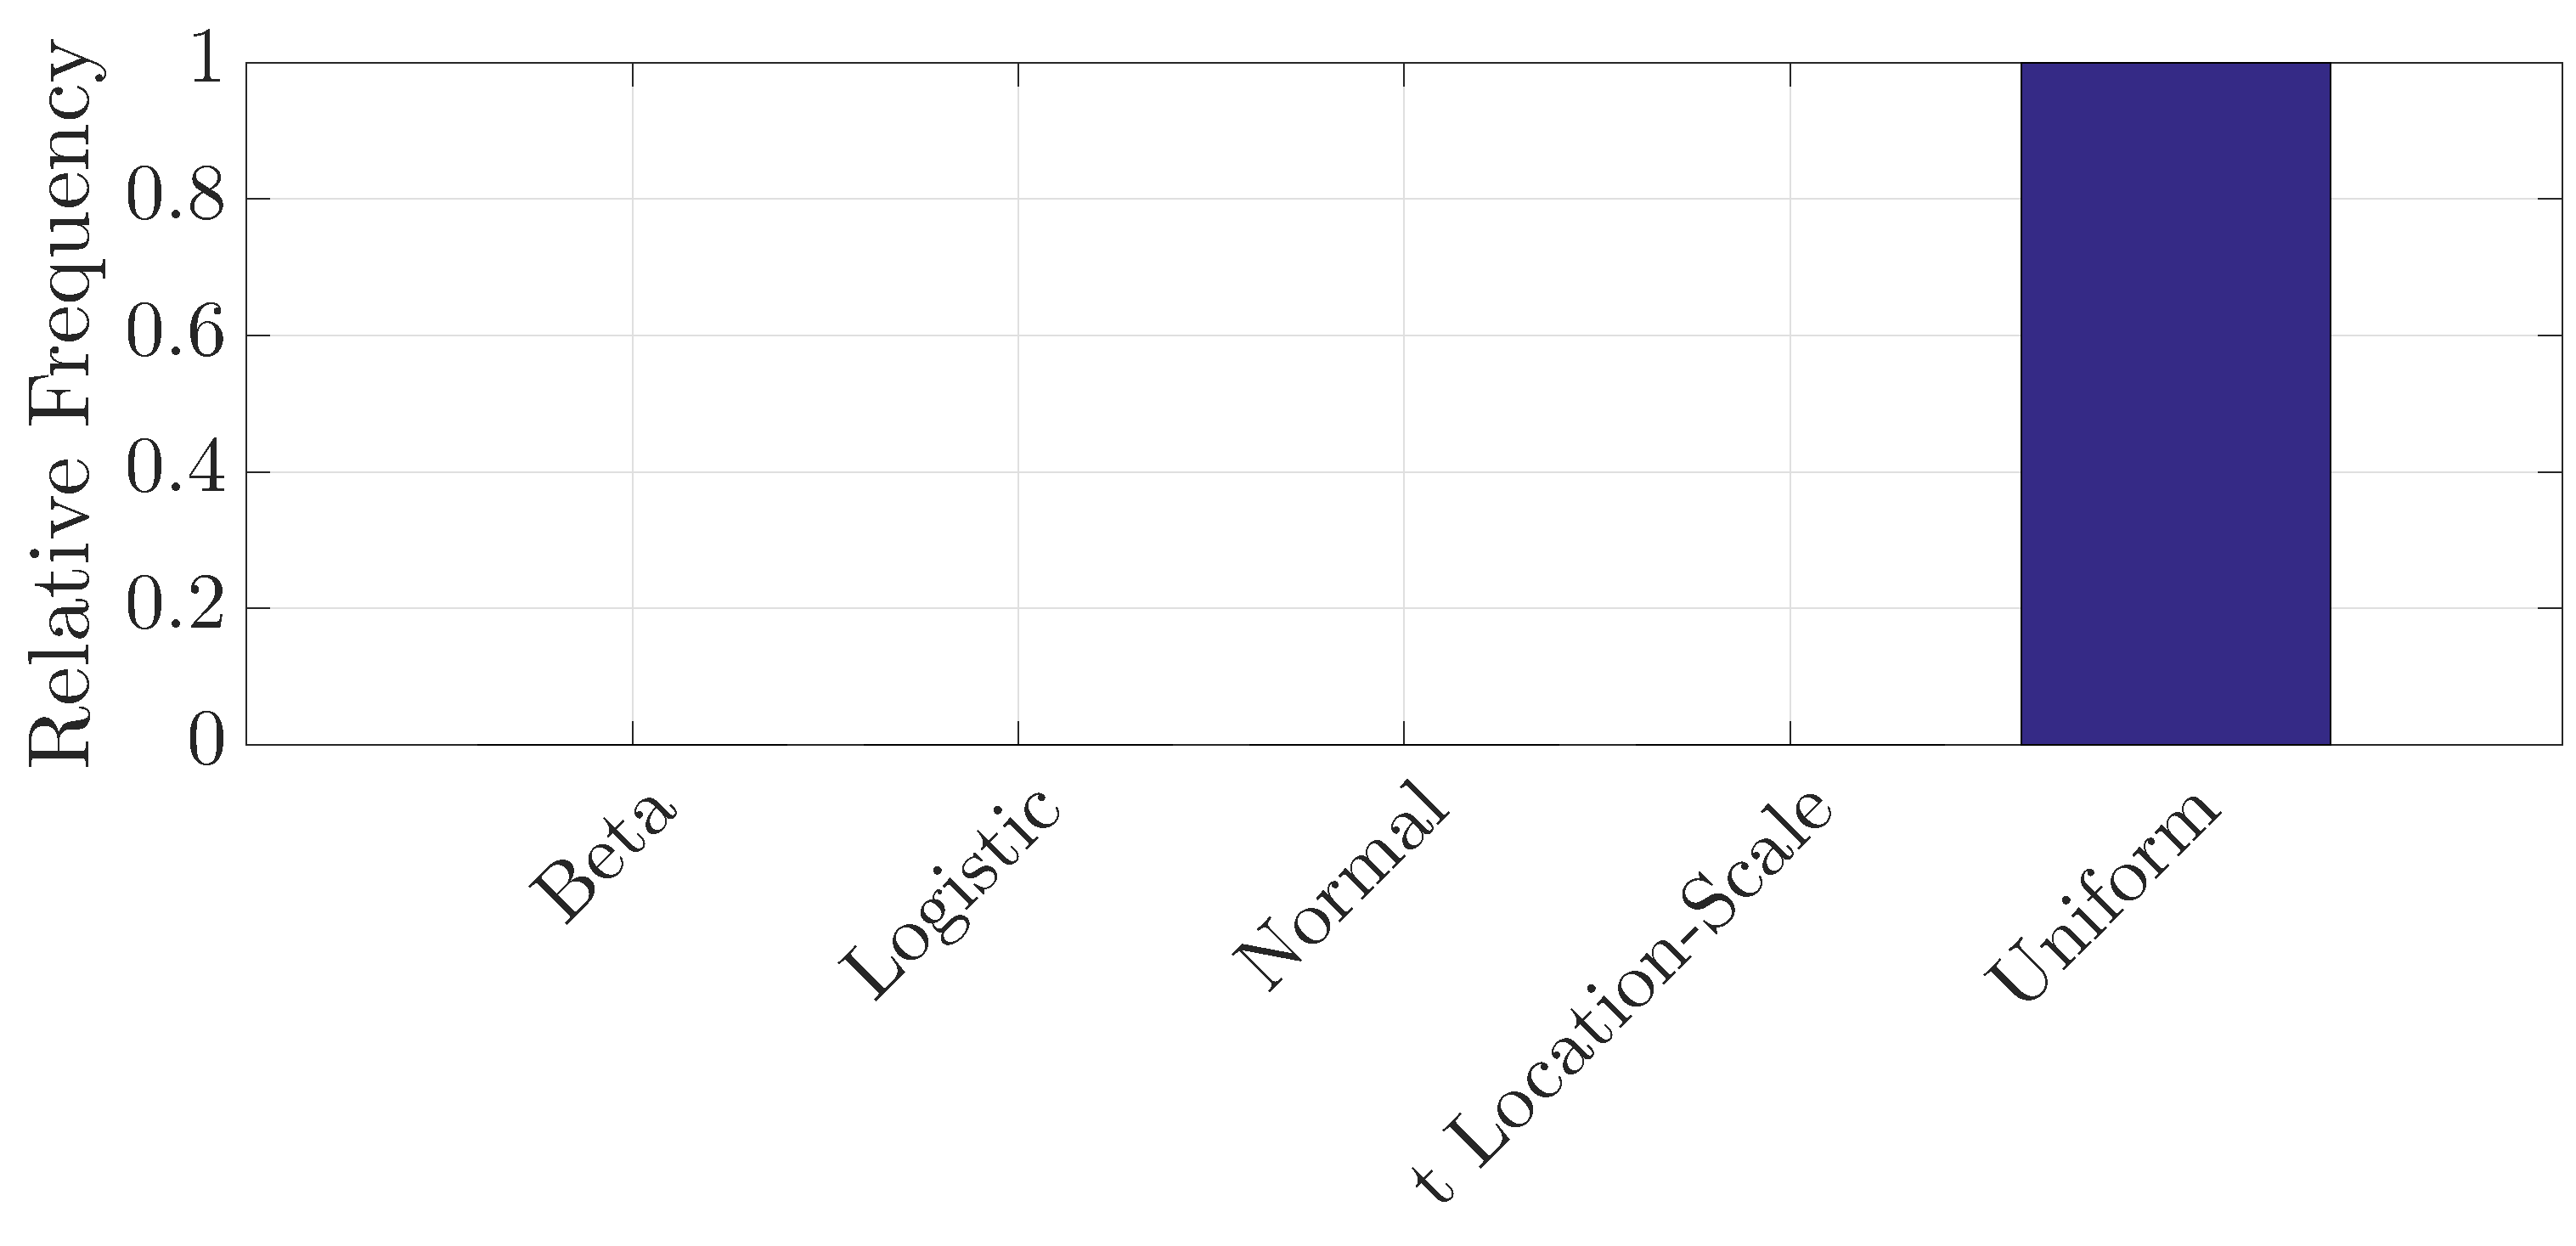
\includegraphics[width=0.9\textwidth]{images/Phase_percent.eps}
	\caption{The relative frequency associated with the chosen statistical distribution that best models CFR phase in accord with the adopted criteria.}
	\label{Phase_percent}
\end{figure}

\begin{figure}[h!]
	\centering
	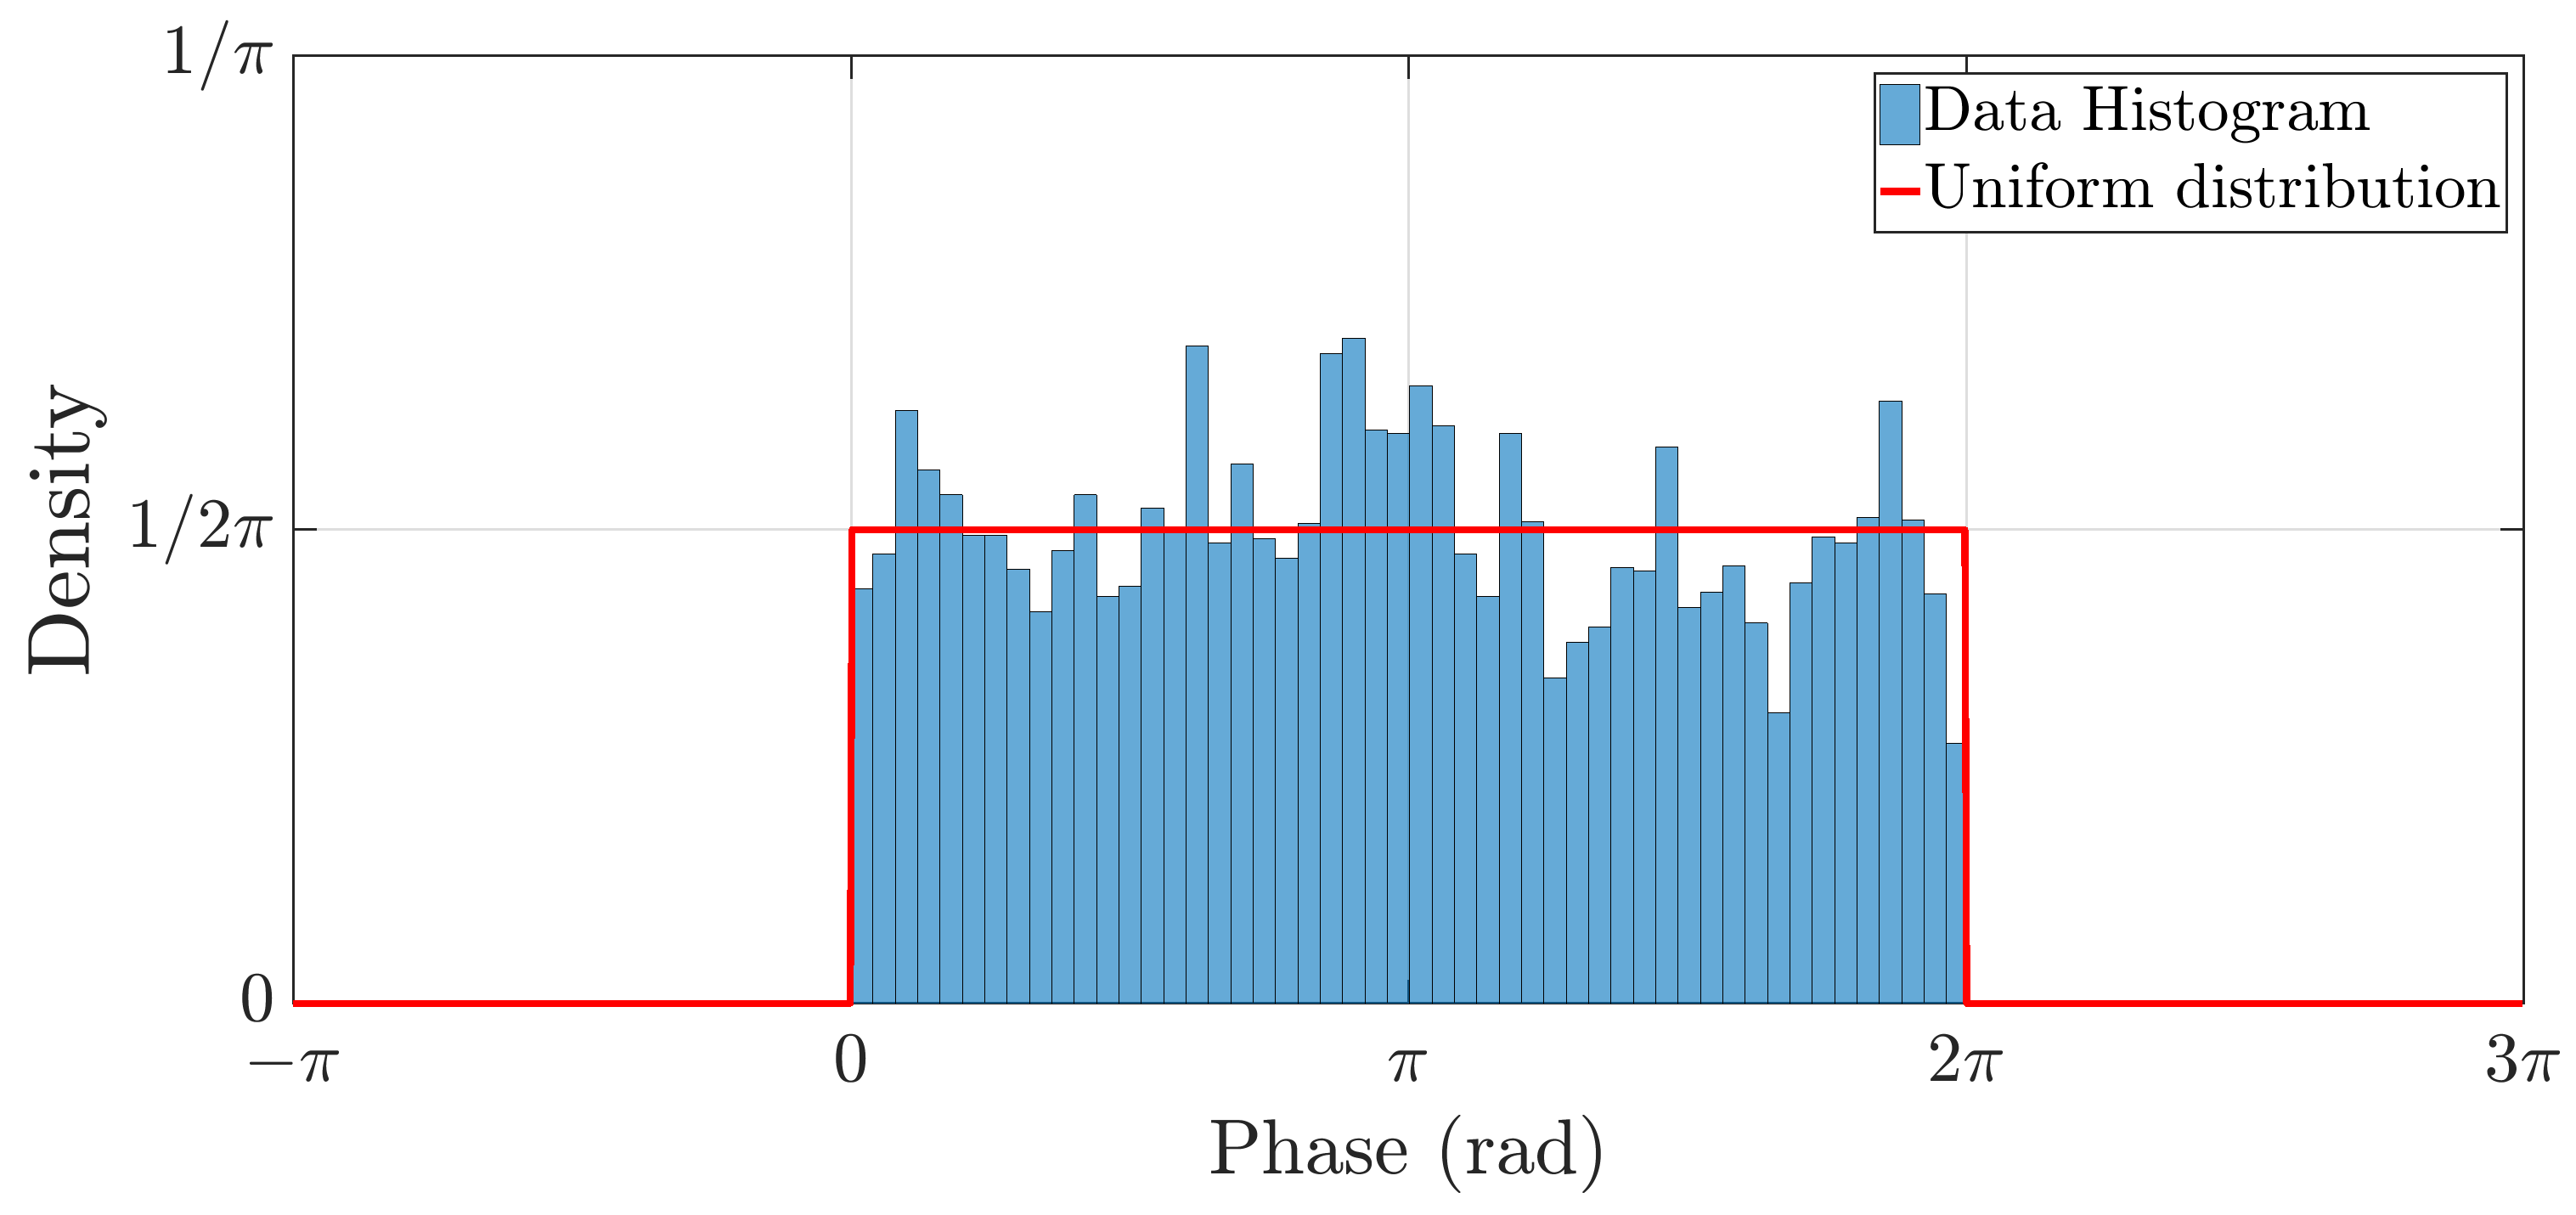
\includegraphics[width=0.9\textwidth]{images/Phase_hist_2.eps}
	\caption{The relative frequency of the phase of the valid CFR estimates at the sample $k$ = 1067 ($k\Delta f= 52.1$ MHz) using the Uniform distribution.}
	\label{phase_example}
\end{figure}

\begin{figure}[h!]
	\centering
	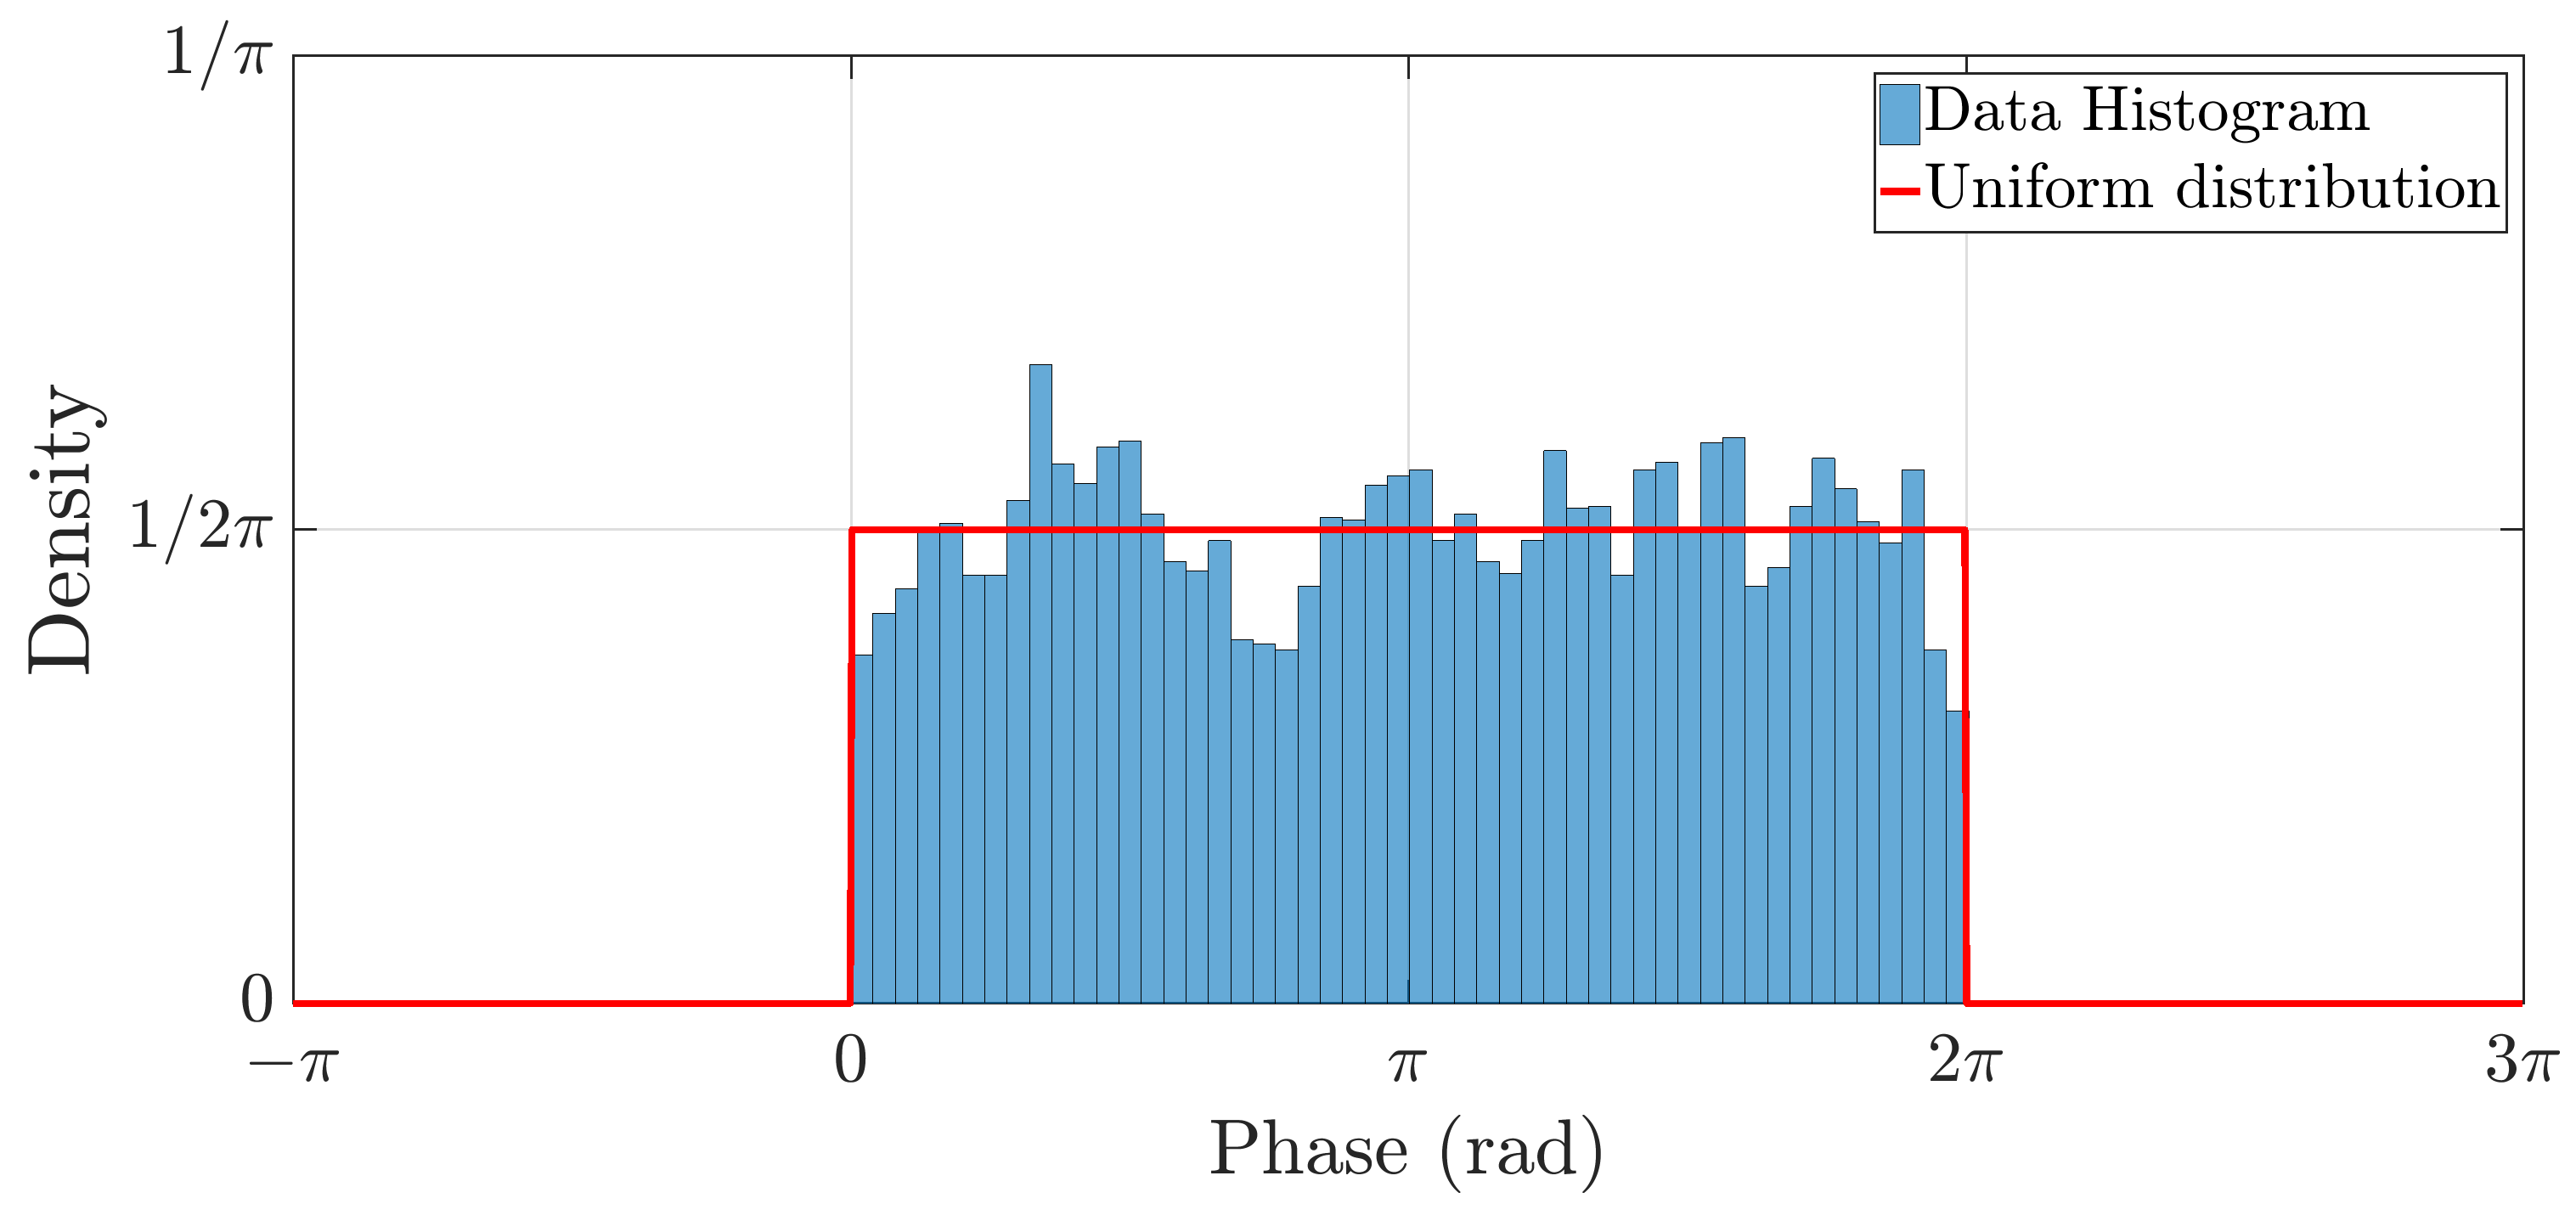
\includegraphics[width=0.9\textwidth]{images/Phase_hist2_2.eps}
	\caption{The relative frequency of the phase of the valid CFR estimates at the sample $k$ = 1600 ($k\Delta f= 78.1$ MHz) using the Uniform distribution.}
	\label{phase_example2}
\end{figure}

In summary, the use of the proposed enhanced statistical modeling method, see Chapter \ref{Proposal}, for modeling the \ac{CFR} of in-home \ac{PLC} channels showed that its magnitude can be modeled by the Beta distribution, with parameters value changing as the frequency varies. As a result, the magnitude function of \ac{CFR} of in-home \ac{PLC} channels is a non-stationary random process. This result is different from previous works that had suggested the Log-normal or Rayleigh distributions, with fixed parameters values, to model this magnitude, see \cite{Galli:Wireline,RayleighPLC}. In other words, the attained results for the Brazilian in-home \ac{PLC} channels shows that previous statistical modeling may not be suitable for the Brazilian residences. The statistical analyses has also verified that the phase component of in-home \ac{PLC} channels can be modeled by the Uniform distribution with fixed parameters as frequency varies, thus denoting that the phase function  of \ac{CFR} of in-home \ac{PLC} channels is a stationary random process.

%%%%%%%%%%%%%%%%%%%%%%%%%%%%%%%%%%%%%%%%%%%%%%%%%%%%%%%%%%%%%%%%%%%%%%%
\section{UNCORRELATED CFR MODEL OF HYBRID PLC-WLC \textit{SHORT-PATH} CHANNELS} \label{sec:NR3}
%%%%%%%%%%%%%%%%%%%%%%%%%%%%%%%%%%%%%%%%%%%%%%%%%%%%%%%%%%%%%%%%%%%%%%%

This section outlines the modeling of the valid \acp{CFR} data set related to in-home hybrid \ac{PLC}-\ac{WLC} \textit{short-path} channels, which were acquired through the measurement campaign described in \cite{thiago:hyb}. Fig. \ref{respfreqsW} portrays five valid and consecutive estimates of the \ac{CFR} magnitude. Each valid \ac{CFR} estimate was obtained by averaging  $L_2$ consecutive \ac{CFR} estimates of the hybrid \ac{PLC}-\ac{WLC} \textit{short-path}. Note that the channel attenuation ranges from approximately $-40$~dB up to $-10$~dB and, in addition, a small time-varying behavior during a time interval shorter than $550\mu$s is observed, once each valid \ac{CFR} estimate covers a time interval equal to $\Delta T = L_2 T_{sym} \approx 115.2\mu$s and, as a consequence, $5\Delta T = 576\mu$s. 

\begin{figure}[h]
	\centering
	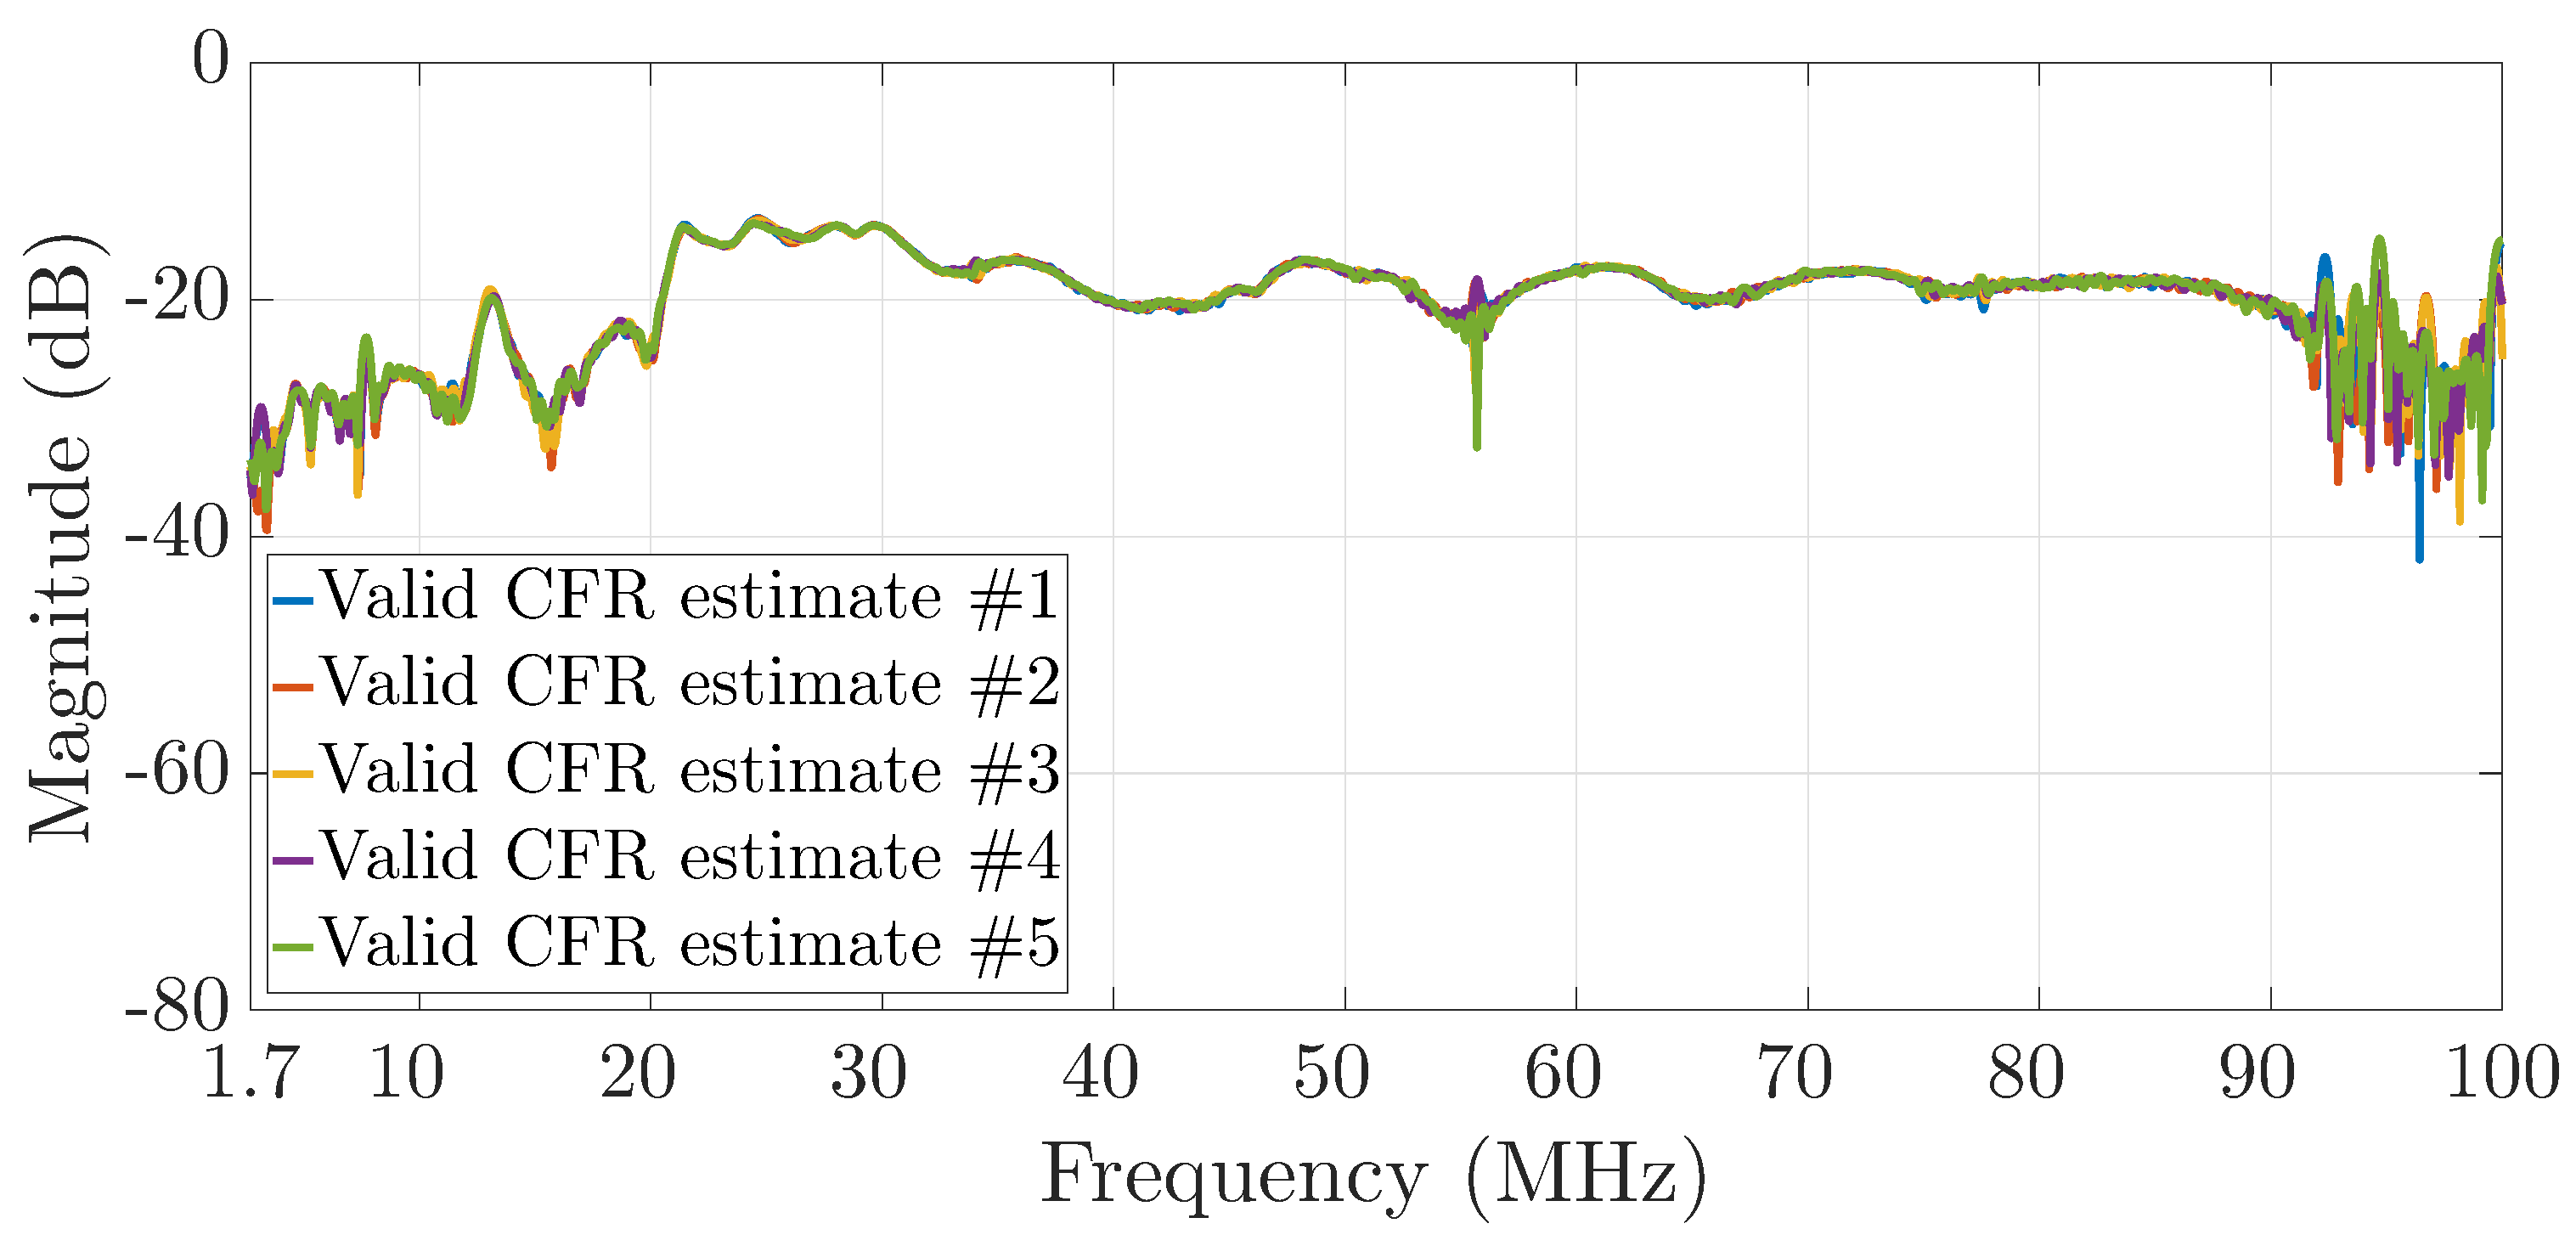
\includegraphics[width=0.9\textwidth]{images/respfreqsW.eps}
	\caption{Five consecutive and valid CFR Magnitudes of the measured in-home PLC channel.}
	\label{respfreqsW}
\end{figure}

Fig. \ref{MAG_percentsW} illustrates the relative frequency of statistical distributions that had modeled the magnitude of the hybrid \ac{PLC}-\ac{WLC} \textit{short-path} \ac{CFR} estimates. On these plots, it is noticeable a statistical distribution that models the majority of the magnitudes, once that in 54\% of the \ac{CFR} estimates the Log-normal distribution resulted in the best model. However, another different statistical distribution stand out as possible candidate to model the \ac{CFR} magnitudes, since in 30\% of the \ac{CFR} estimates, the Gamma distribution offered the best modeling. 

\begin{figure}[h!]
	\centering
	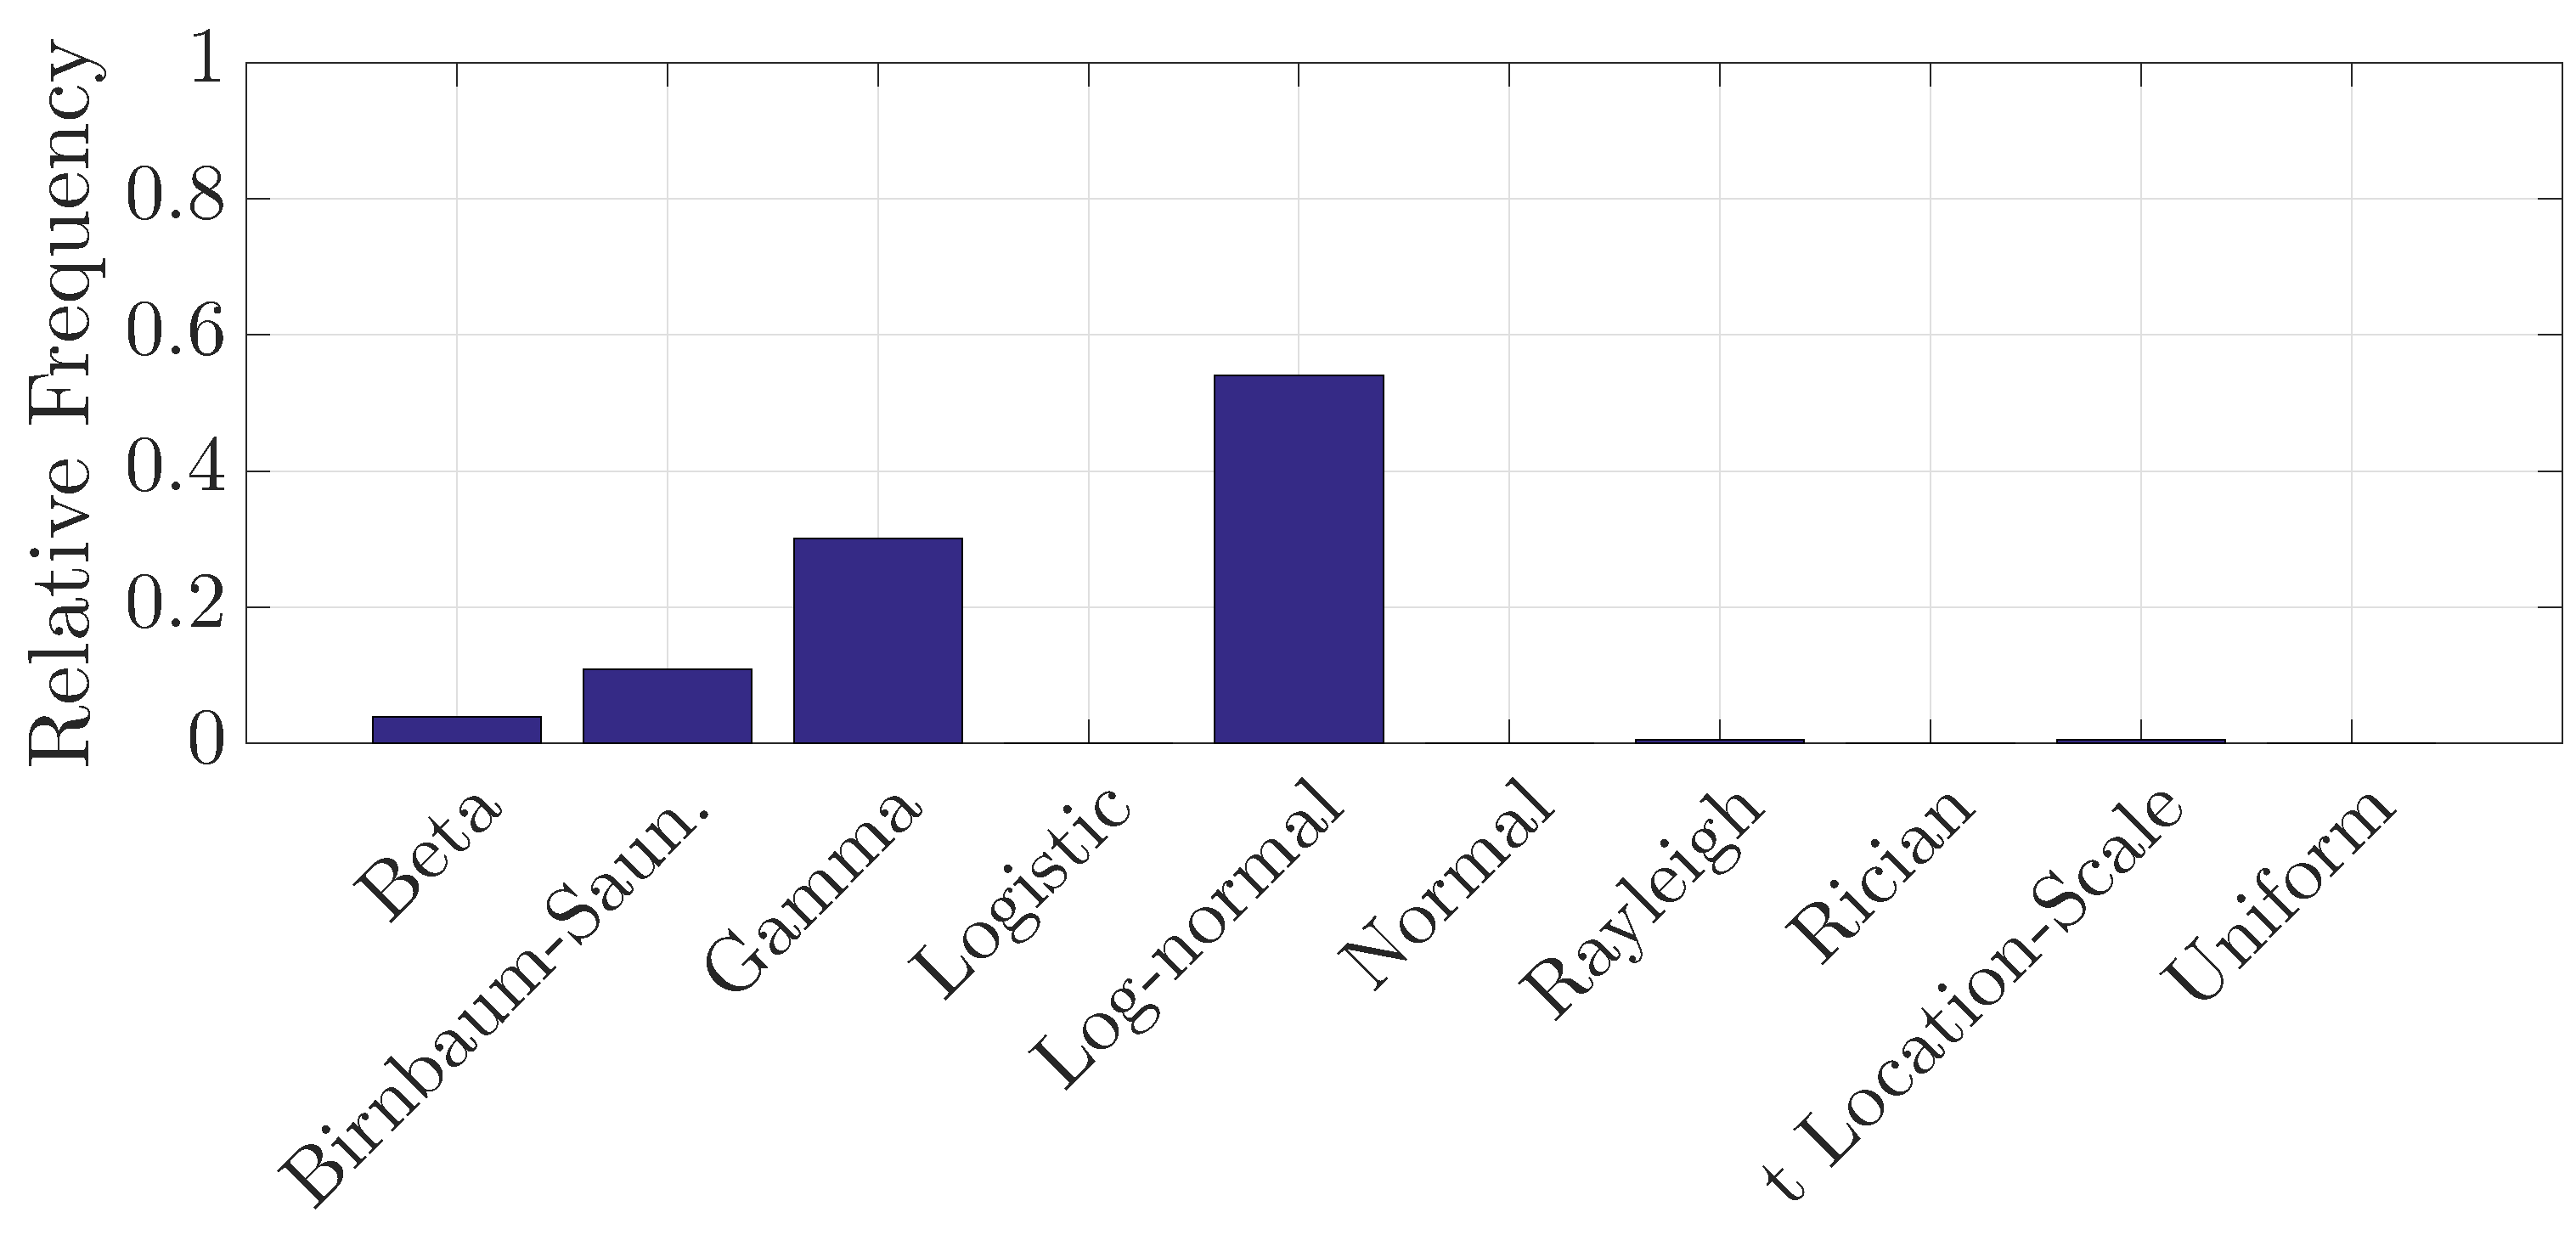
\includegraphics[width=0.9\textwidth]{images/MAG_percentsW.eps}
	\caption{The relative frequency associated with the chosen statistical distribution that best models the CFR magnitude in accord with the adopted criteria.}
	\label{MAG_percentsW}
\end{figure}

Similarly to subsection \ref{sec:NR2}, the log-likelihood ratio $\rho_{MLE} (f)$ (\ref{eq:log-lik}) was used in order to evaluate which of the two distributions is the best choice to model the magnitude component of the \ac{CFR} estimates. Fig. \ref{fig:Log_likesW} shows the values of  $\rho_{MLE}(f)$ for the two best statistical distributions candidates to model the magnitude of the valid \ac{CFR} estimates. Once again a red dashed line was used to indicate the threshold value of $1.2$, under which the statistical distribution can be considered good enough to model the magnitude of \ac{CFR}. These curves emphasize that both Log-normal and Gamma distributions achieved the minimum ratio over the \ac{MLE} criteria, in this scenario, the Log-normal distribution was chosen due to its greater occurrence as the best model for the \ac{PLC}-\ac{WLC} \textit{short-path} \ac{CFR} magnitudes, as portrayed in Fig. \ref{MAG_percentsW}. In other words, the magnitude of the valid \ac{CFR} estimates of in-home hybrid \ac{PLC}-\ac{WLC} \textit{short-path} channels is modeled by using only one statistical distribution (i.e., the Log-normal distribution).

%\begin{figure}[h!]
%	\centering
%	\psfrag{AAA}[c][c][1.3]{$\rho_{MLE} (f)$}
%	\subfloat[]{\includegraphics[width=0.9\textwidth]{images/Log_LogNsW.eps}}\\~\\
%	\psfrag{AAA}[c][c][1.3]{$\rho_{MLE} (f)$}
%	\subfloat[]{\includegraphics[width=0.9\textwidth]{images/Log_GammasW.eps}}\\~\\
%	\caption{The log-likelihood ratio for the following statistical distributions: (a) Log-normal, (b) Gamma.}
%	\label{fig:Log_likesW}
%\end{figure}

\begin{figure}[h!]
	\centering
	\psfrag{AAA}[c][c][1.3]{$\rho_{MLE} (f)$}
	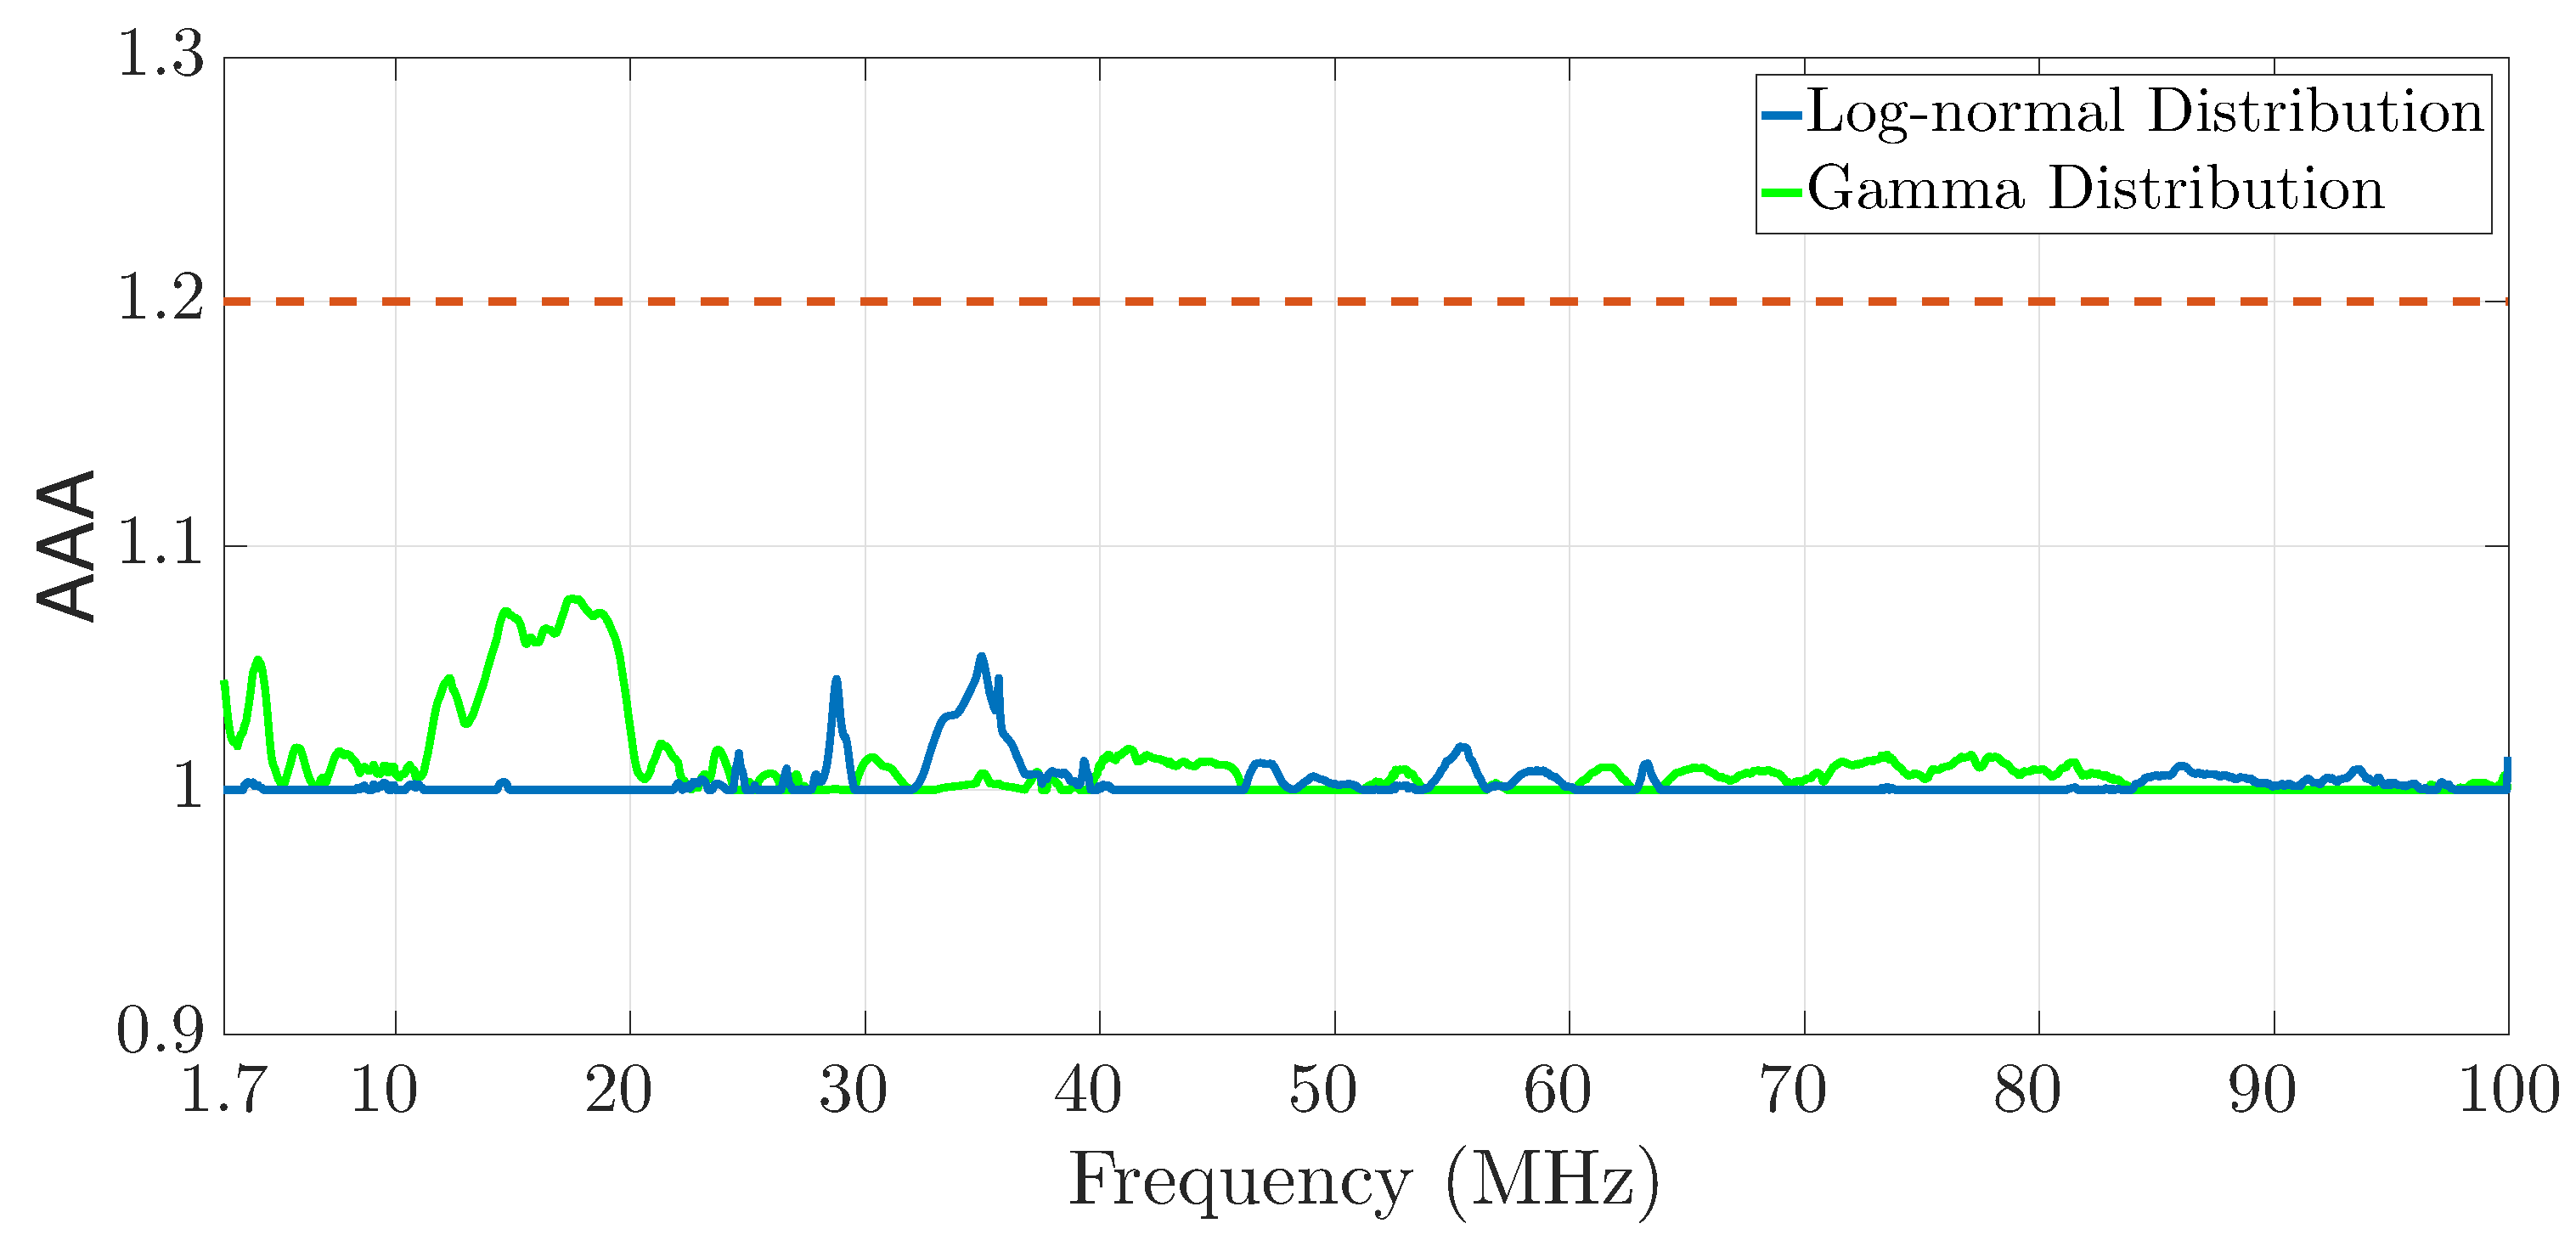
\includegraphics[width=0.9\textwidth]{images/Log_Lognormal_GammasW.eps}
	\caption{The log-likelihood ratio for the following statistical distributions: Log-normal, Gamma.}
	\label{fig:Log_likesW}
\end{figure}


The statistical analysis of the magnitude of the valid \ac{PLC}-\ac{WLC} \textit{short-path} \ac{CFR} estimates showed that the parameters of the Log-normal distribution assume different values as frequency changes. If $\mathcal{C}_{k} = \{\zeta_1[k],\zeta_2[k]\}$ is the set of parameters for the statistical distribution modeling the magnitude of the valid \ac{CFR} estimates of \ac{PLC}-\ac{WLC} \textit{short-path} channels, where $k=0,1,\cdots,N-1$,  $\zeta_1[k] = \mu[k]$ and $\zeta_2[k] = \sigma[k]$, are the two parameters ($U=2$) of the Log-normal distribution, named mean and standard deviation respectively, associated with the $k$-th sample of the valid \ac{CFR}. Then, Fig. \ref{mag_examplesW} and Fig. \ref{mag_example2sW} illustrates the statistical models for two different values of frequency: $f=50.78$~MHz ($k=1040 \rightarrow f = 1040\Delta f$) and $f=80.57$~MHz ($k=1650 \rightarrow f = 1650\Delta f$), respectively. The parameters of the Log-normal distribution are  $\mu(1040 \Delta f) = \zeta_1[1040]=-4.0117$ and $\sigma( 1040 \Delta f) = \zeta_2[1040] = 0.5903$; $\mu(1650 \Delta f) = \zeta_1[1650] = -5.034$ and $\sigma( 1650 \Delta f) = \zeta_2[1650]=0.82$ for $f=50.78$~MHz and $f=80.57$~MHz, respectively.

\begin{figure}[h!]
	\centering
	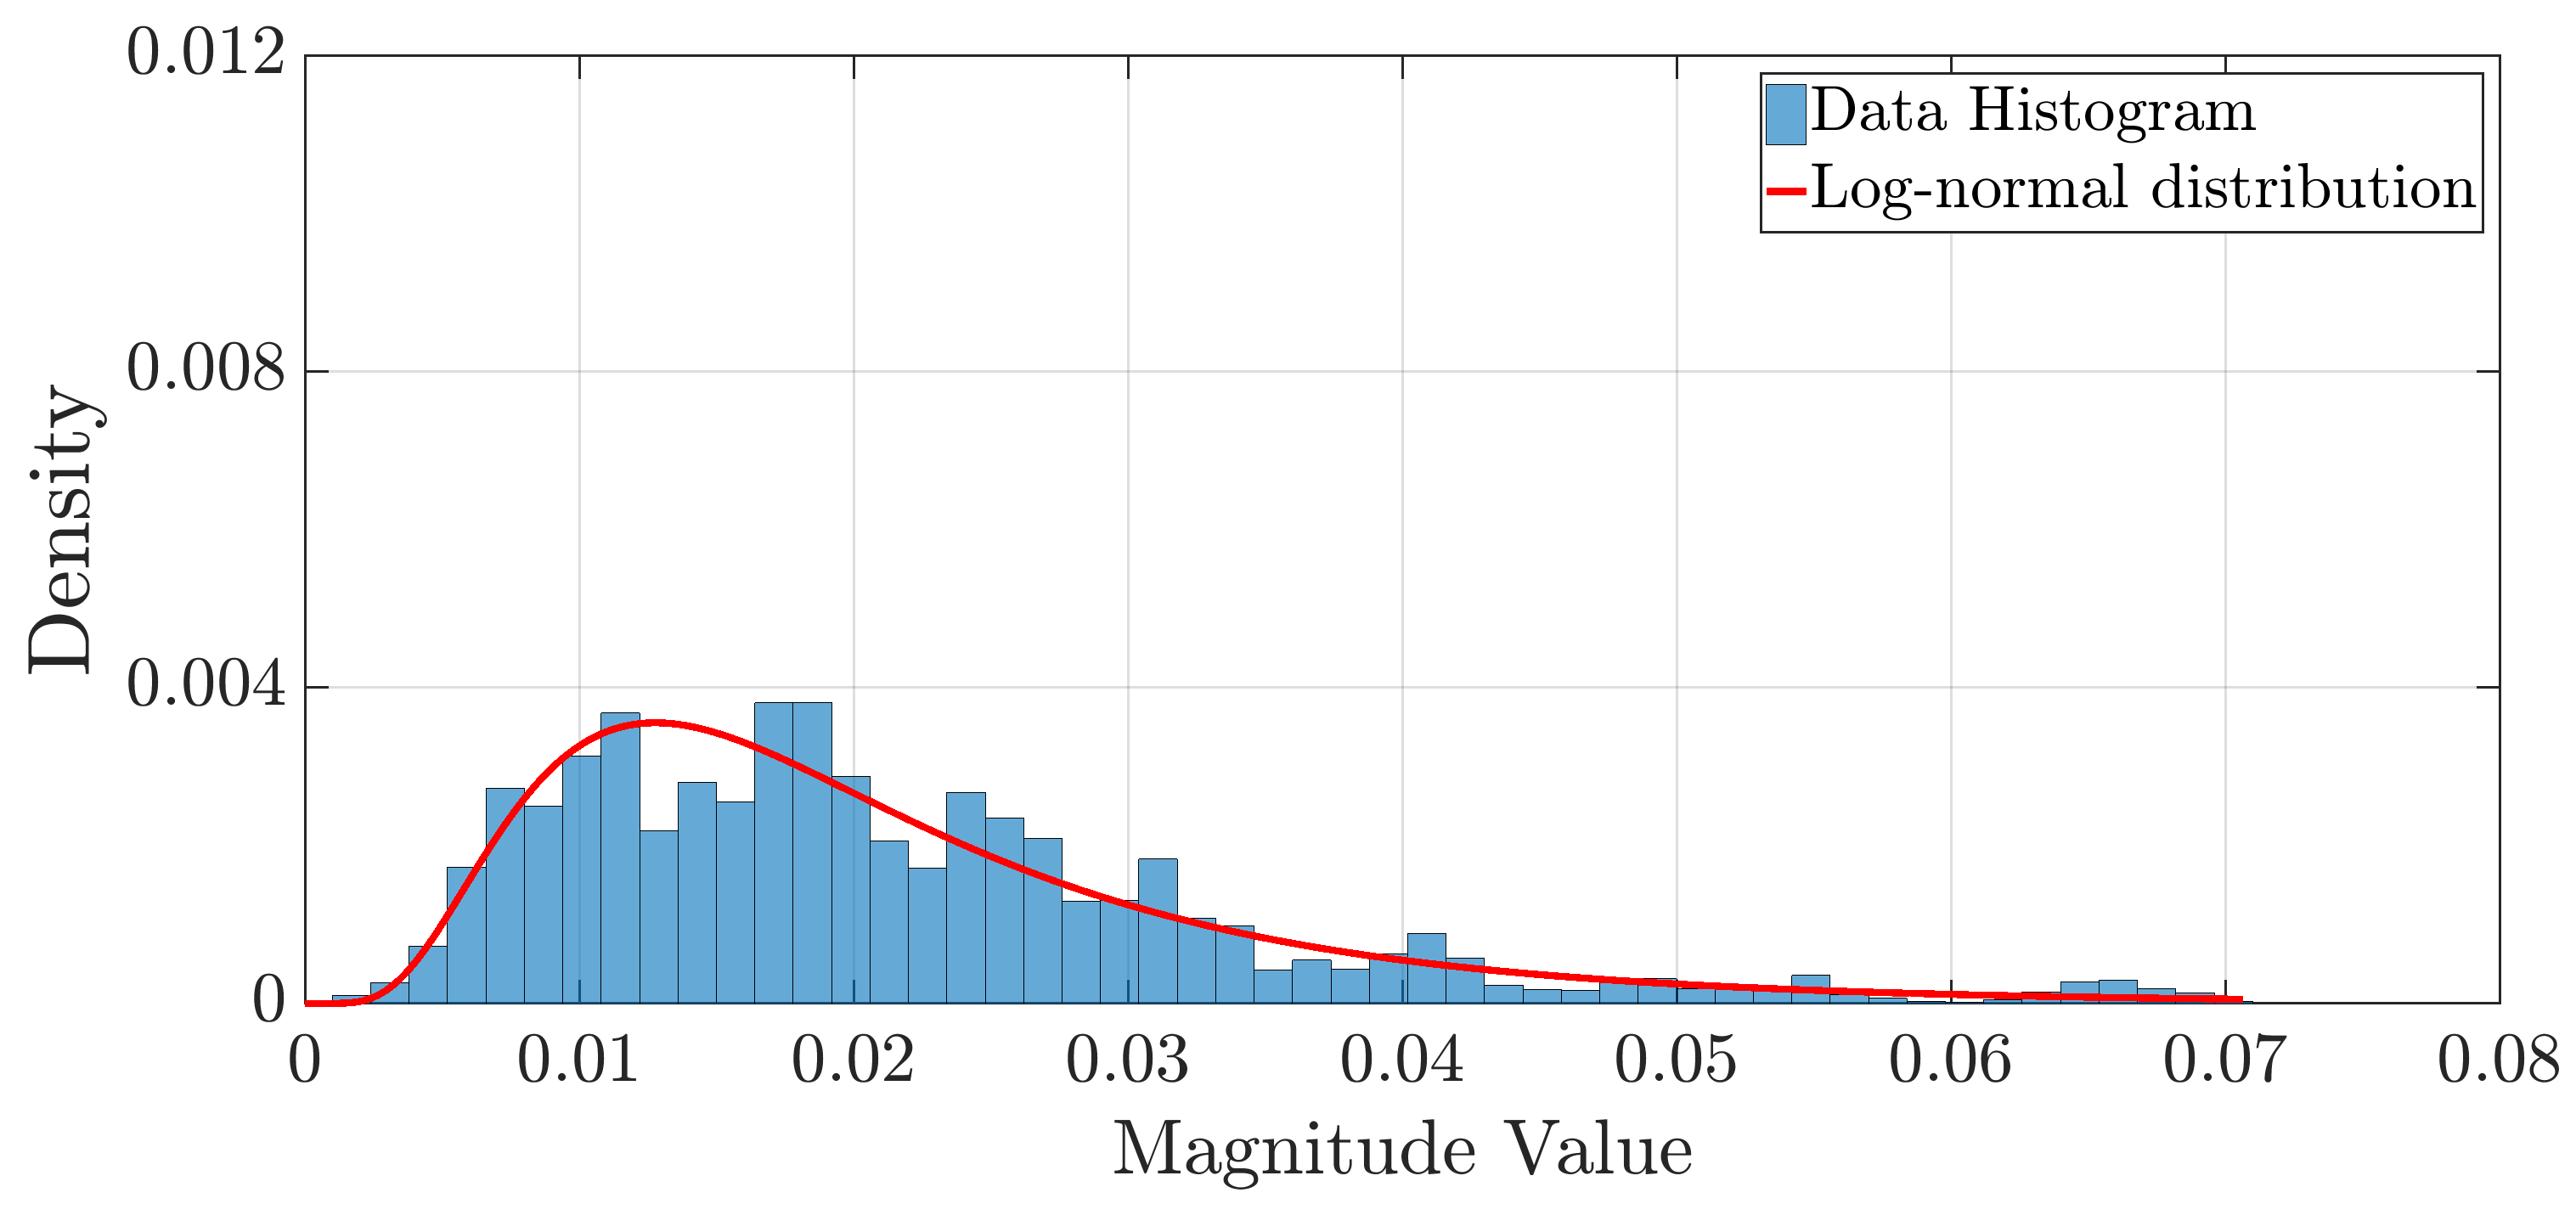
\includegraphics[width=0.9\textwidth]{images/Mag_histsW_2.eps}
	\caption{The relative frequency of the magnitude of the valid CFR estimates at the sample $k = 1040$ ($k\Delta f= 50.78$~MHz) and the modeling based on the Log-normal distribution.}
	\label{mag_examplesW}
\end{figure}

\begin{figure}[h!]
	\centering
	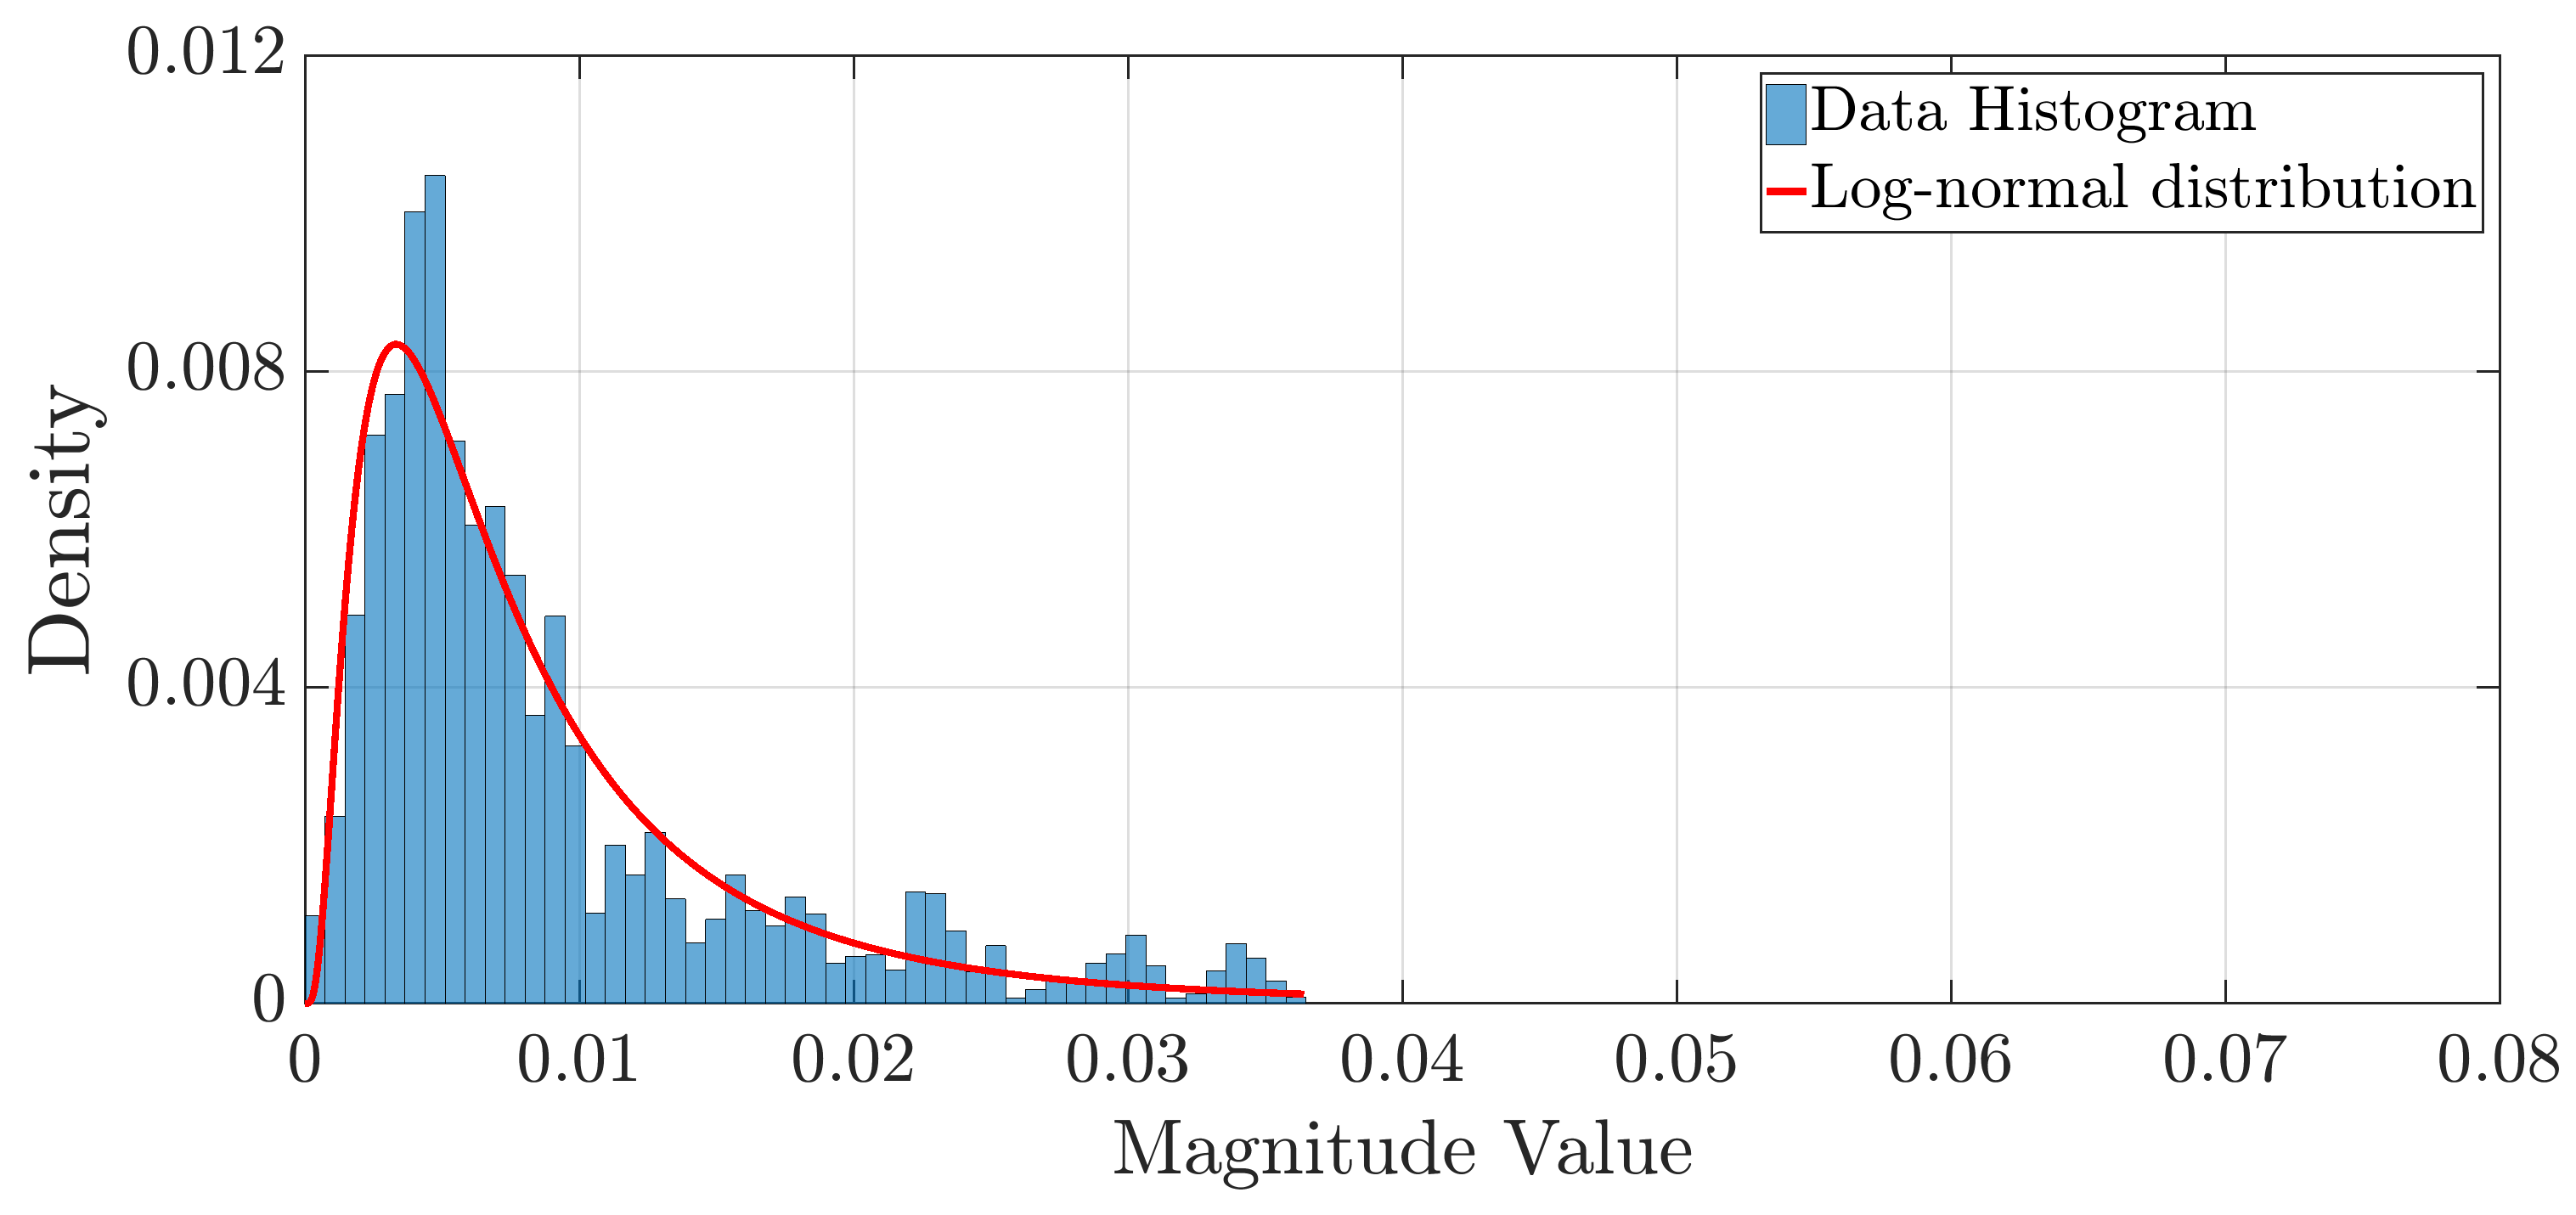
\includegraphics[width=0.9\textwidth]{images/Mag_hist2sW_2.eps}
	\caption{ The relative frequency of the magnitude of the valid CFR estimates at the sample $k = 1650$ ($k\Delta f= 80.57$~MHz) and the modeling based on the Log-normal distribution.}
	\label{mag_example2sW}
\end{figure}

Fig. \ref{fig:boundsSW} illustrates the \ac{MSE} results in terms of the number of subbands for the in-home hybrid \ac{PLC}-\ac{WLC} \textit{short-path} channels. On these plots is possible to notice that independently of the chosen criterion to select the non-uniformity of the subbands, the \ac{MSE} value does not change significantly as the number of subbands becomes higher than $15$ and  due to a trade off between the precision of the interpolation and the complexity of computing it, $L=15$ was chosen as the number of subbands. By interpolating the parameters values $\mu[k]$ and $\sigma[k]$ of the Log-normal distributions associated with the model of the \ac{CFR} of the hybrid \ac{PLC}-\ac{WLC} \textit{short-path} channel using $L=15$ subbands and the Algorithm \ref{Algo2}, the continuous curves of parameters $\hat{\mu}(\omega)$ and $\hat{\sigma}(\omega)$ are yielded. Finally, the curves $\hat{\mu}(f)$ and $\hat{\sigma}(f)$ are easily obtained once $\omega \in [0,\pi)$ directly corresponds to the frequency band between $0$ and $100$~MHz. Figs. \ref{Fit_alfasW} and \ref{Fit_betasW} portrays the curves for the parameters $\mu(f)$ and $\sigma(f)$, which are obtained by applying frequency domain interpolation technique detailed in \cite{mitra} and the curves obtained by using the cubic Spline interpolation with $L=15$ subbands. Similar to previous subsections, Table \ref{table_alfasW} in Appendix \ref{ap:e} lists the cubic Spline coefficients for modeling the parameter $\mu(f)$, of the valid \ac{CFR} magnitude while Table \ref{table_betasW}, in Appendix \ref{ap:e} as well, covers the cubic Spline coefficients for modeling the parameter $\sigma(f)$. Overall, it is important to point out that the Log-normal distribution and its coefficients waveform $\hat{\mu(f)}$ and $\hat{\sigma(f)}$ define the random process representing the magnitude of the \ac{CFR} of the in-home hybrid \ac{PLC}-\ac{WLC} \textit{short-path} channel.

\begin{figure}[h!]
	\centering
	\subfloat[]{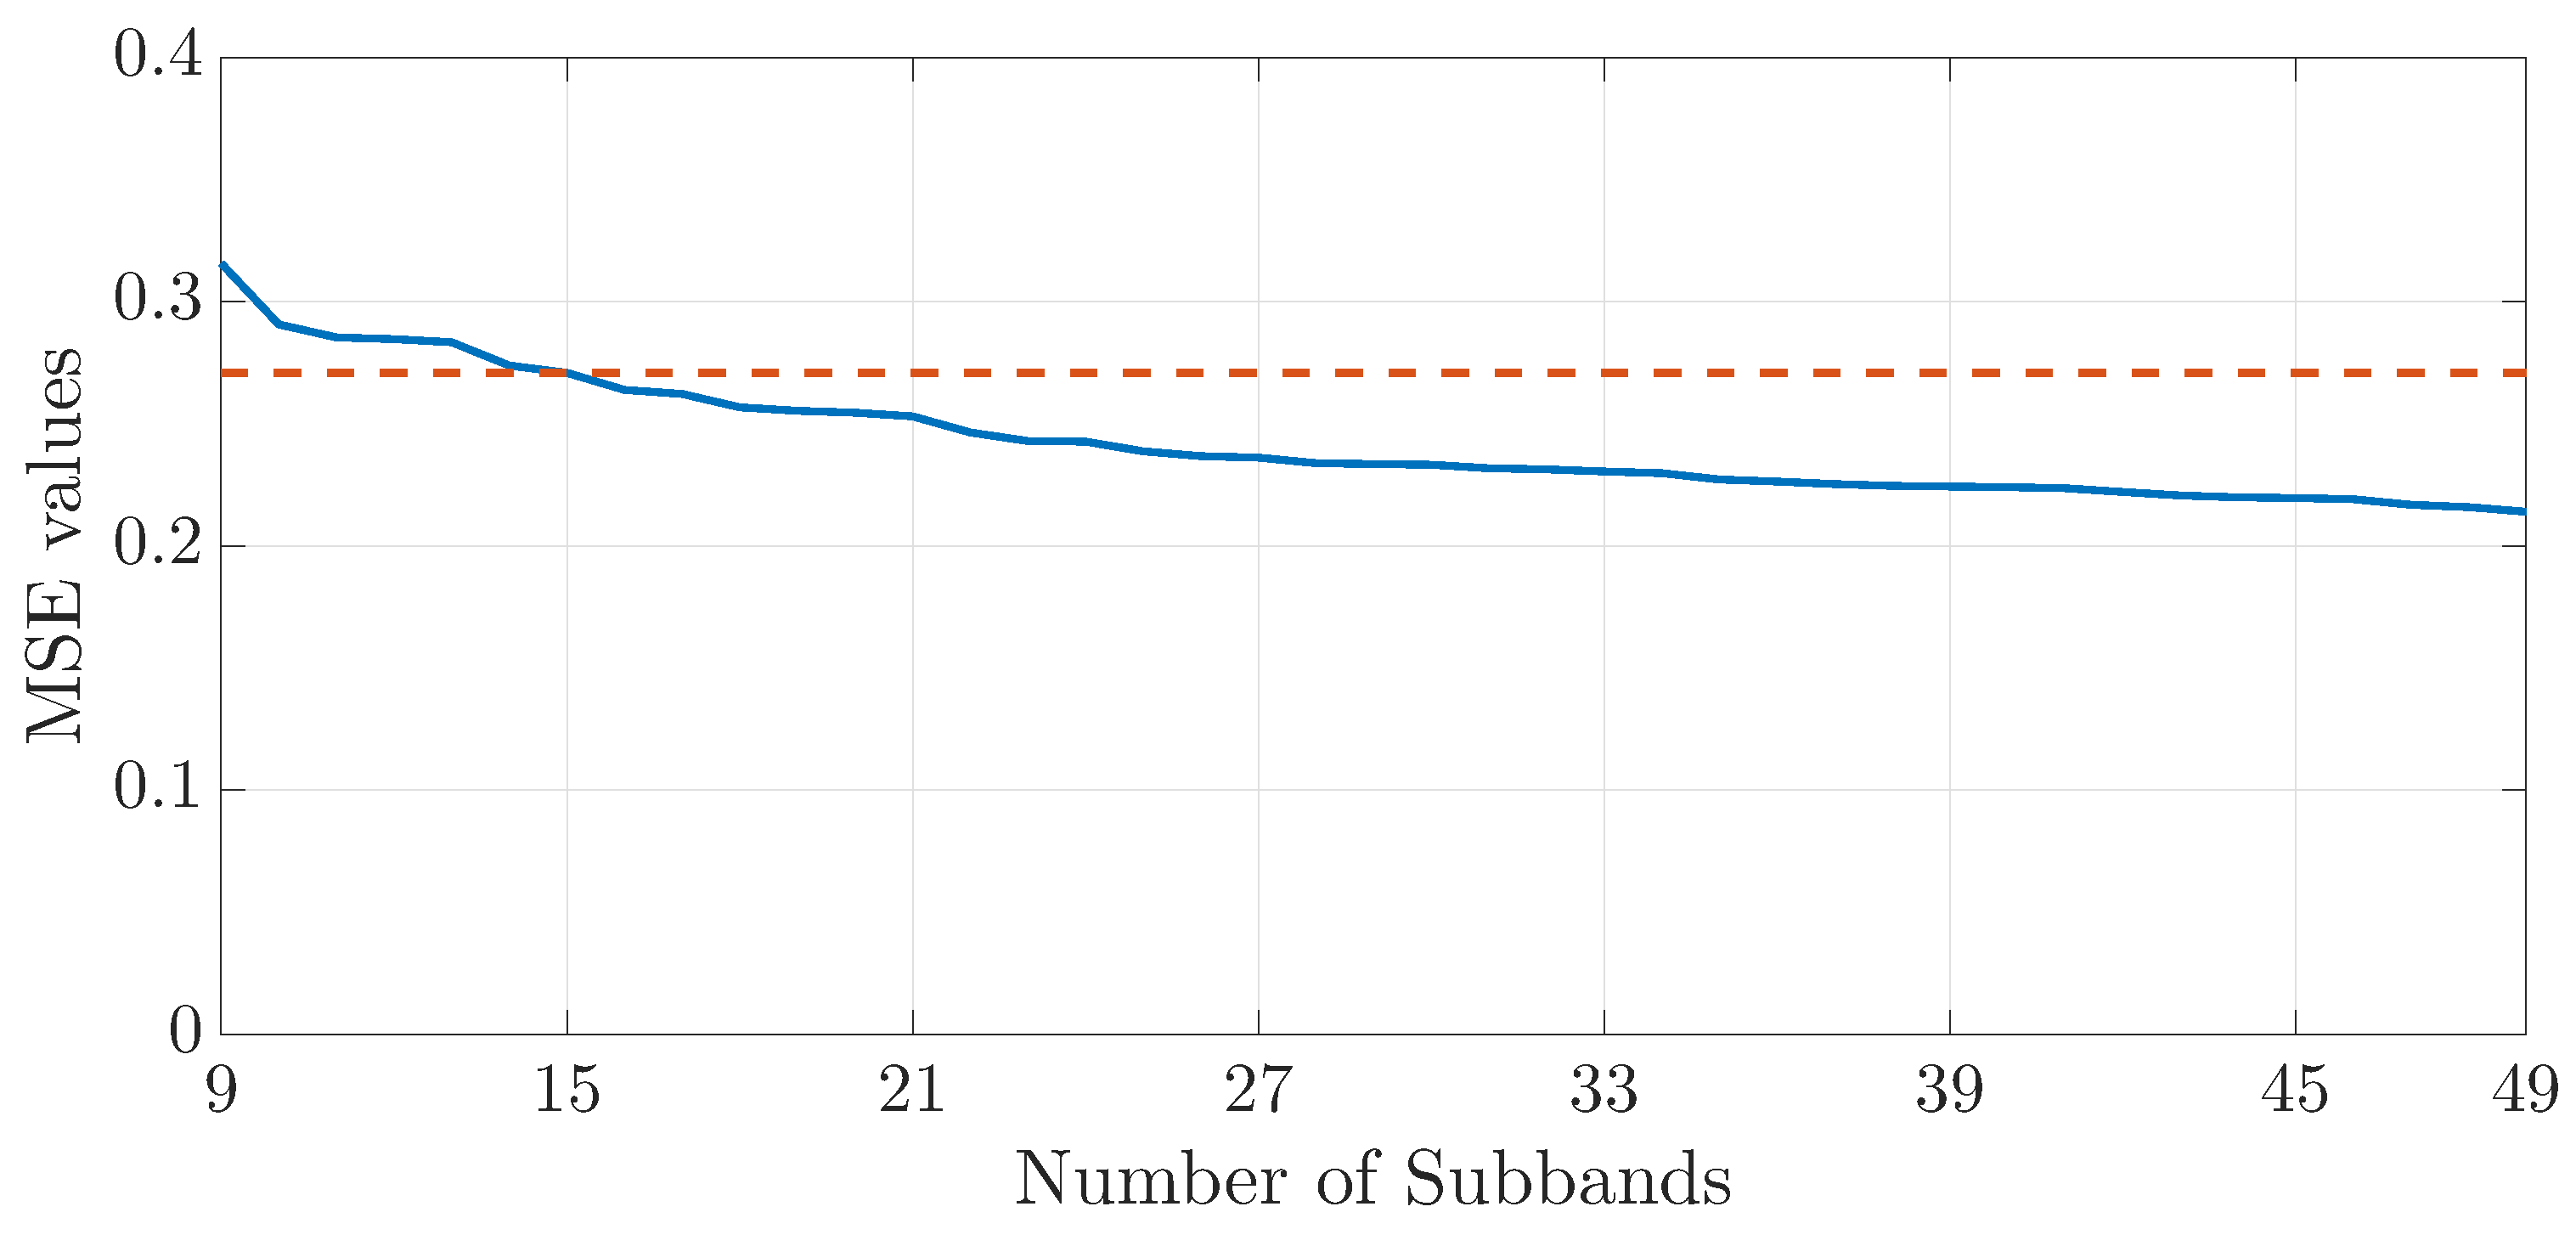
\includegraphics[width=0.9\textwidth]{images/alfasW_bounds.eps}}\\~\\
	\subfloat[]{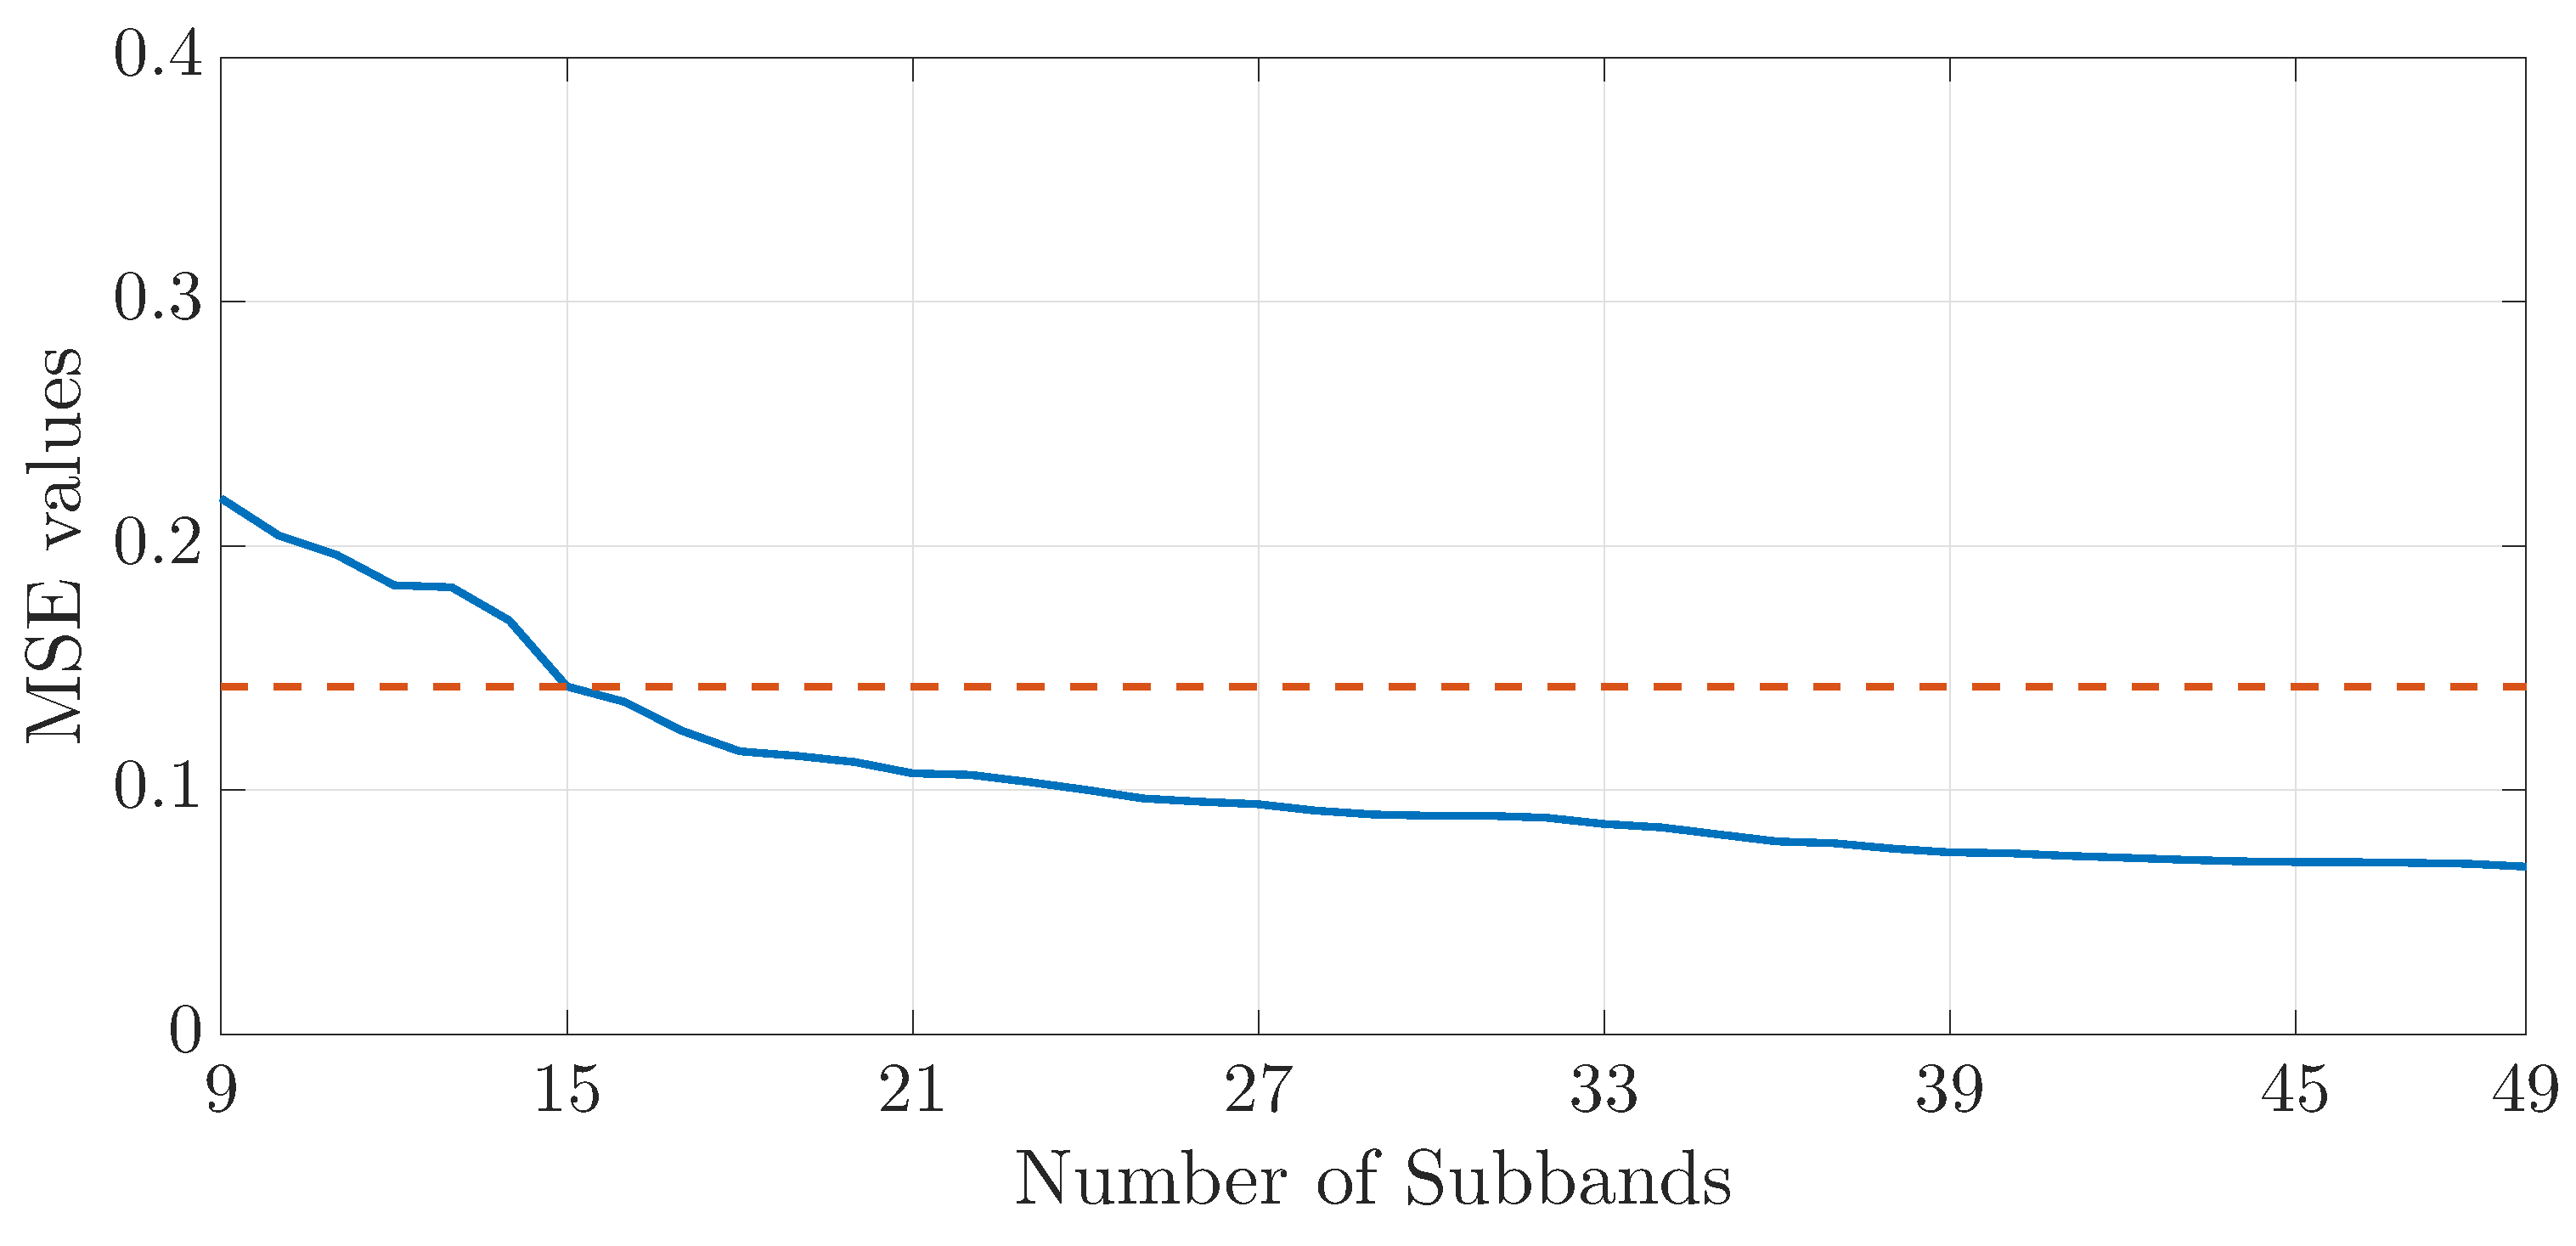
\includegraphics[width=0.9\textwidth]{images/betasW_bounds.eps}}\\~\\
	\caption{The MSE values for the parameters from \textit{short-path} scenario: (a) $\mu$ parameter, (b) $\sigma$ parameter.}
	\label{fig:boundsSW}
\end{figure}

\begin{figure}[h]
	\centering
	\psfrag{Interval Boundsaa}[c][c][1]{Interval Bounds}
	\psfrag{AAA}[c][c][1]{$~~~~~\mu(k \Delta f)$}
	\psfrag{BBB}[c][c][1]{$~\hat{\mu}(f)$}
	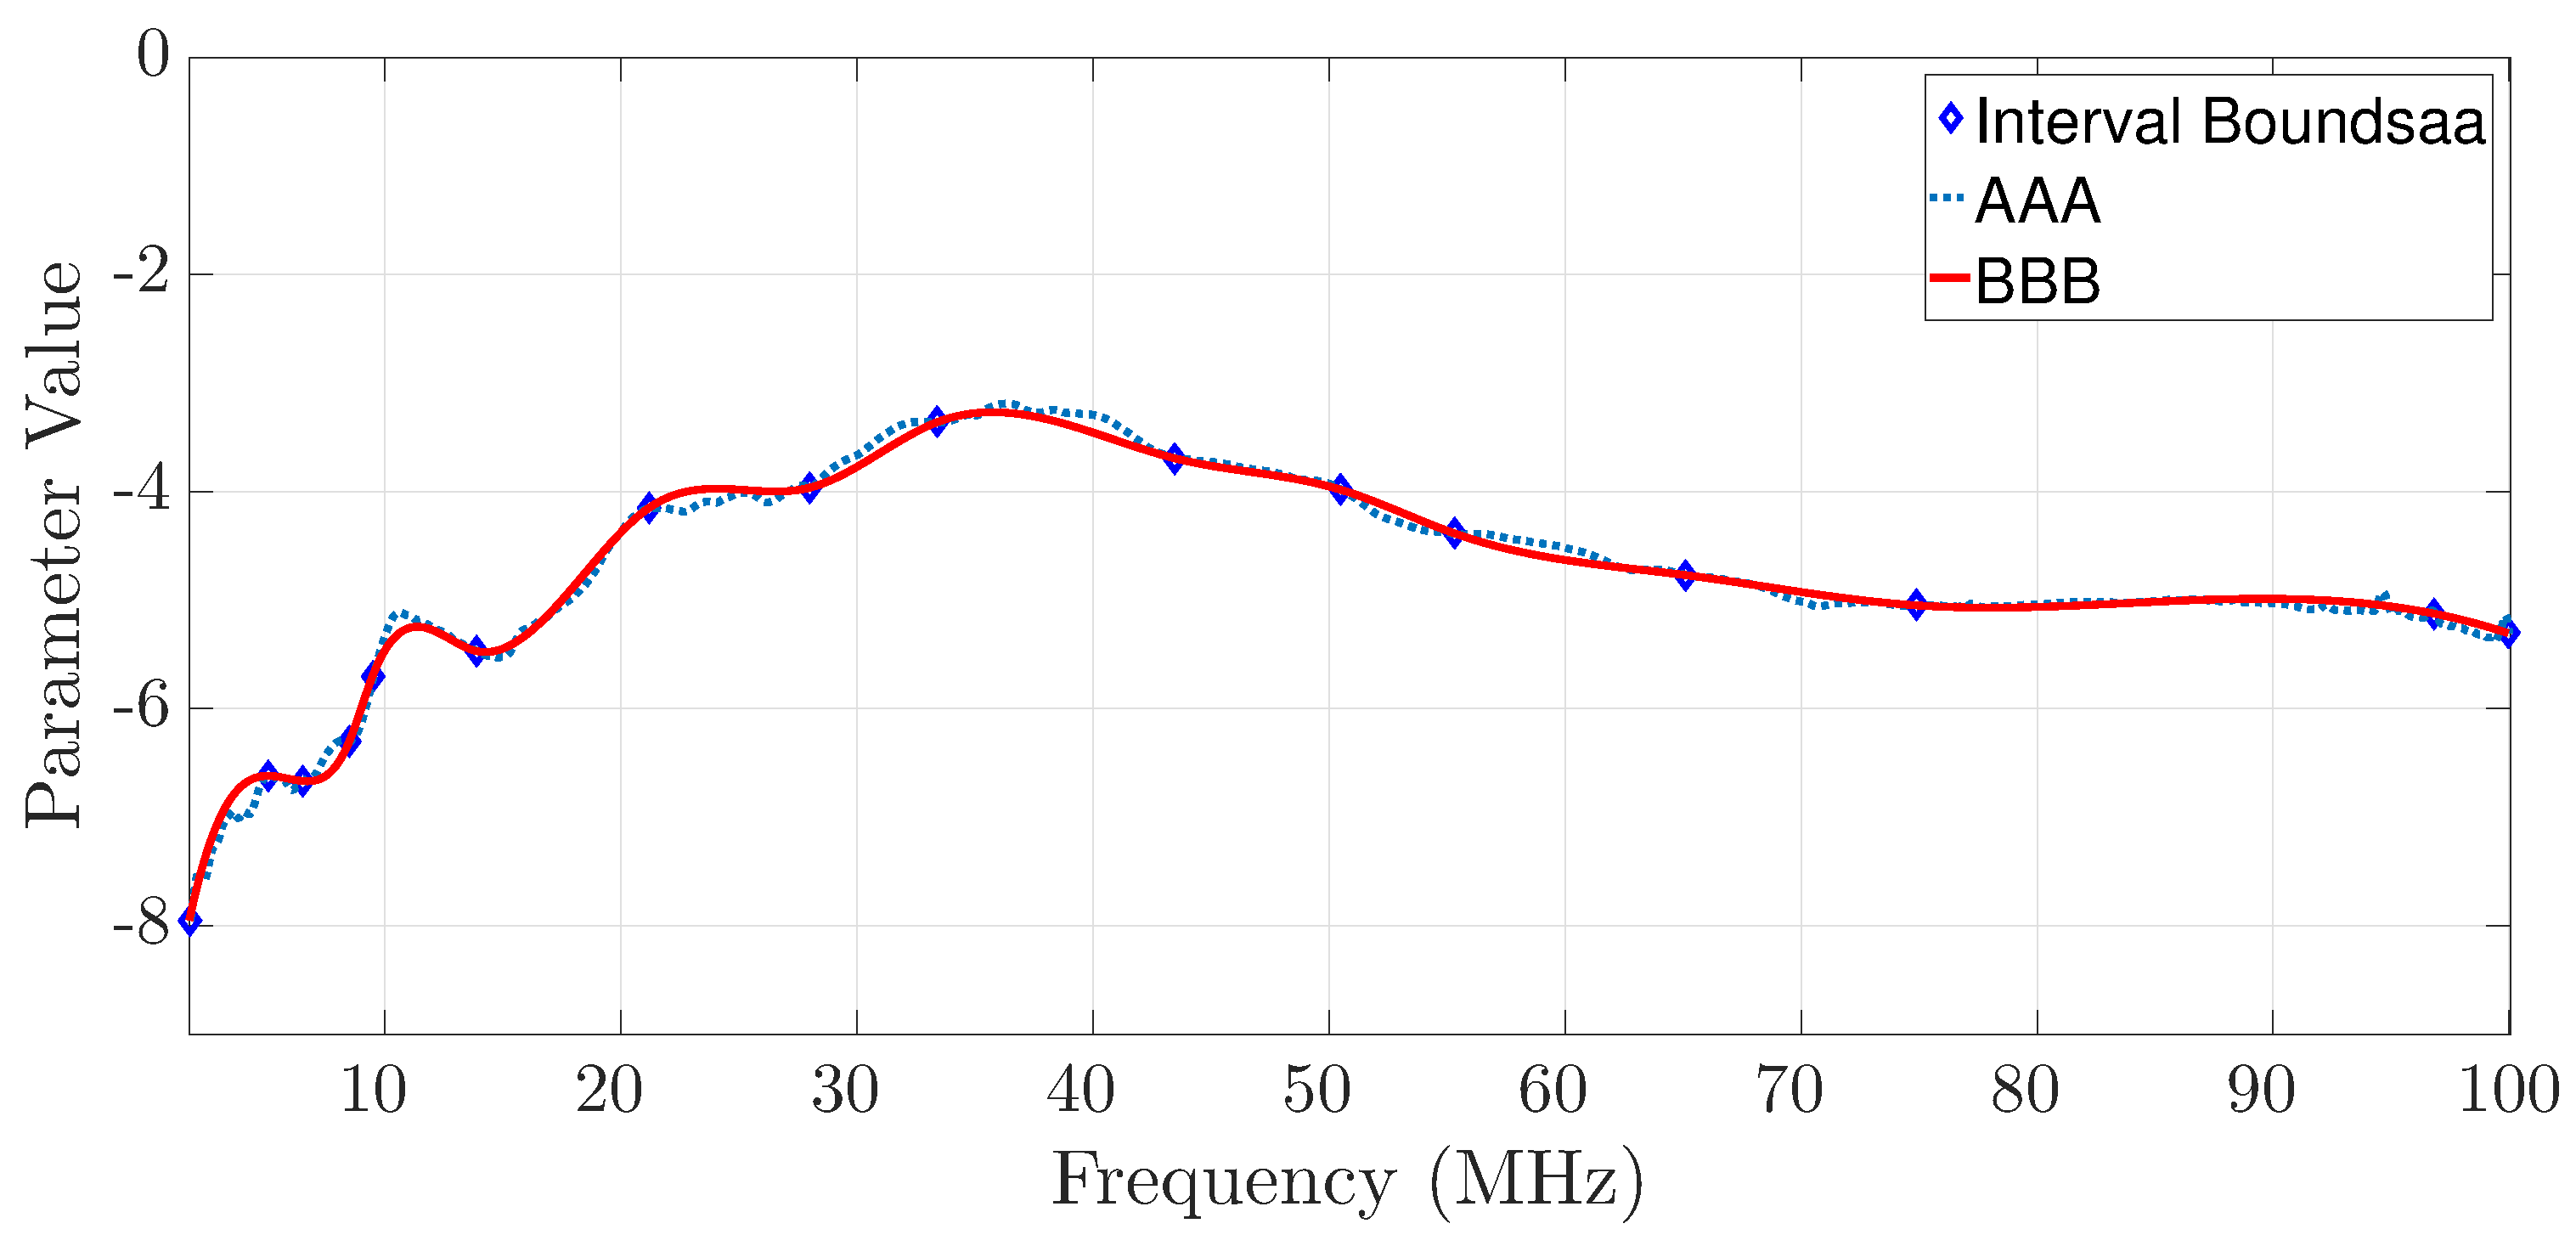
\includegraphics[width=0.92\textwidth]{images/Alfa_fitsW.eps}
	\caption{The result of the interpolation technique based on cubic Splines applied to obtain $\mu(f)=\zeta_1(f)$ for the Log-normal distribution (${\mu}(k \Delta f)$ are the original values of the parameter and $\hat{\mu}(f)$ is the interpolated curve).}
	\label{Fit_alfasW}
\end{figure}

\begin{figure}[h]
	\centering
	\psfrag{Interval Boundsaa}[c][c][1]{Interval Bounds}
	\psfrag{AAA}[c][c][1]{${~~~~~\sigma}(k \Delta f)$}
	\psfrag{BBB}[c][c][1]{$~\hat{\sigma}(f)$}
	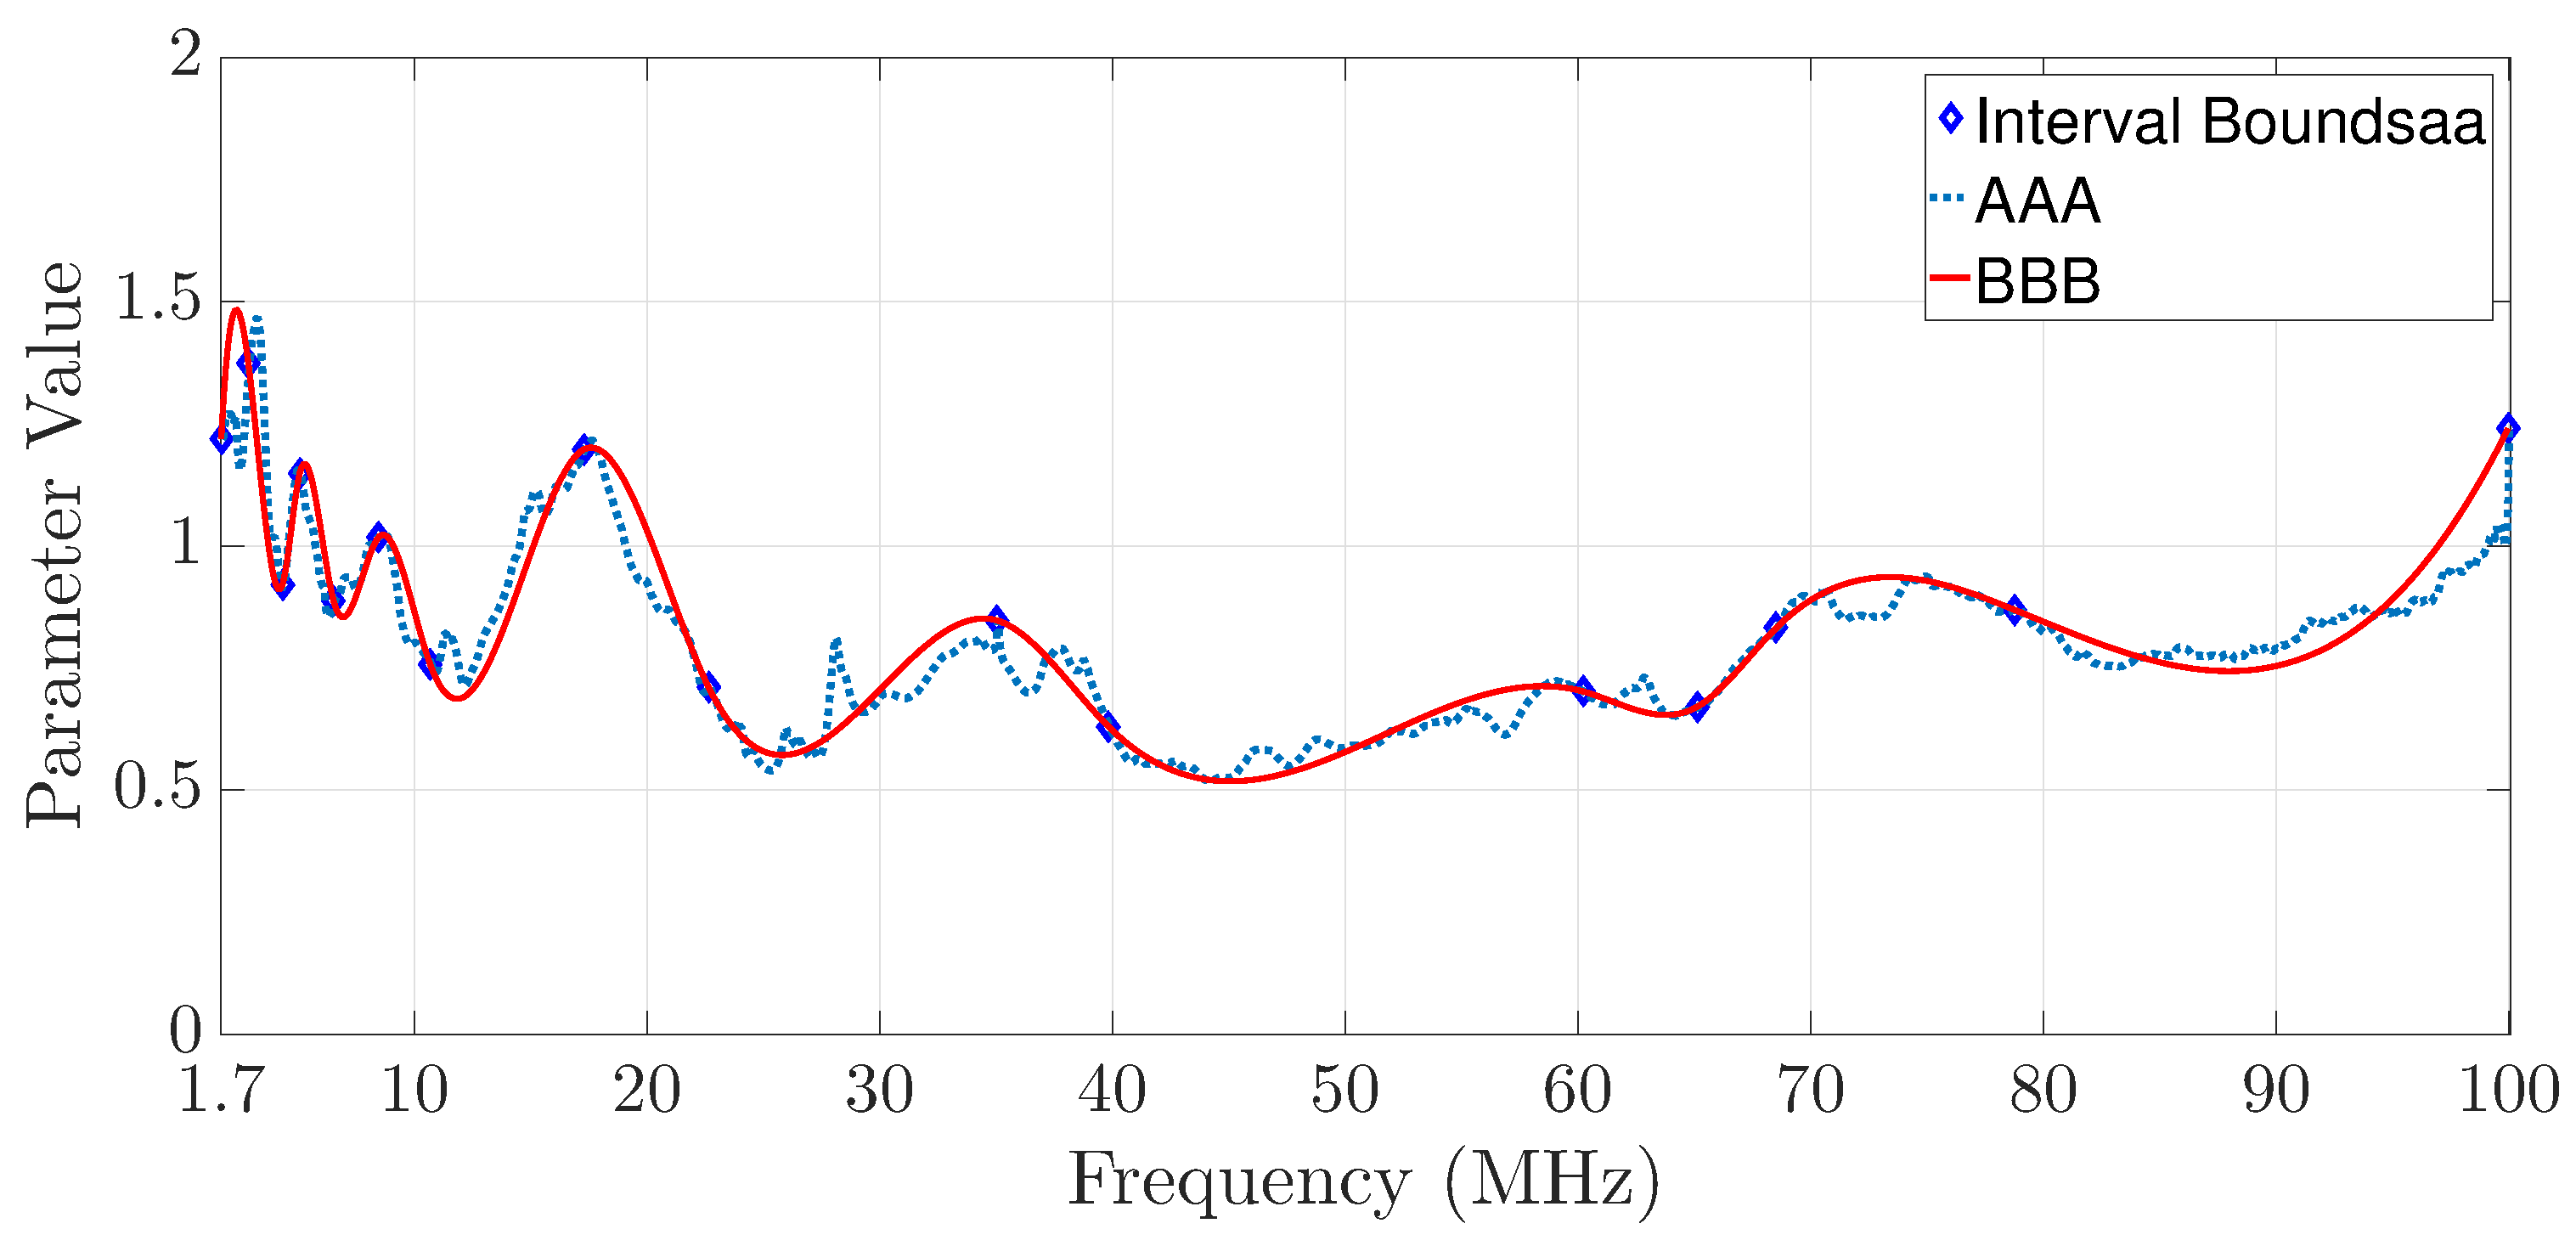
\includegraphics[width=0.9\textwidth]{images/Beta_fitsW.eps}
	\caption{The result of the interpolation technique based on cubic Splines applied to obtain $\sigma(f)=\zeta_2(f)$ for the Log-normal distribution (${\sigma}(k \Delta f)$ are the original values of the parameter and $\hat{\sigma}(f)$ is the interpolated curve).}
	\label{Fit_betasW}
\end{figure}

Fig. \ref{Phase_percentsW} portrays the relative frequency of statistical distributions that had modeled, in accord with the adopted criteria, the phase of the whole set of valid  hybrid \ac{PLC}-\ac{WLC} \textit{short-path} \ac{CFR} estimates. Similarly to the \ac{PLC} \ac{CFR} estimates, on this scenario 100\% of the data set was best modeled by the Uniform distribution and the statistical modeling of the phase of the valid \ac{CFR} estimates have shown that each sample of it can be modeled by the same set of parameters of the Uniform distribution. In other words, $\Theta_k \in [0, 2\pi]$ denotes the interval of values that the phase of the valid \ac{PLC}-\ac{WLC} \textit{short-path} \ac{CFR} estimates can assume and it defines the support for the Uniform distribution. 

Fig. \ref{phase_examplesW} and Fig. \ref{phase_example2sW} shows the statistical models regarding the frequencies $f=50.78$~MHz ($k=1040 \rightarrow f = 1040\Delta f$) and $f=80.57$~MHz ($k=1650 \rightarrow f = 1650\Delta f$), respectively. Independent of the frequency values, the phase model of the valid \ac{CFR} estimates remains the same. As a result, by using the Uniform distribution defined in the interval $[0, 2\pi]$, the random process representing the phase of the in-home hybrid \ac{PLC}-\ac{WLC} \textit{short-path} channel is obtained.

\begin{figure}[h!]
	\centering
	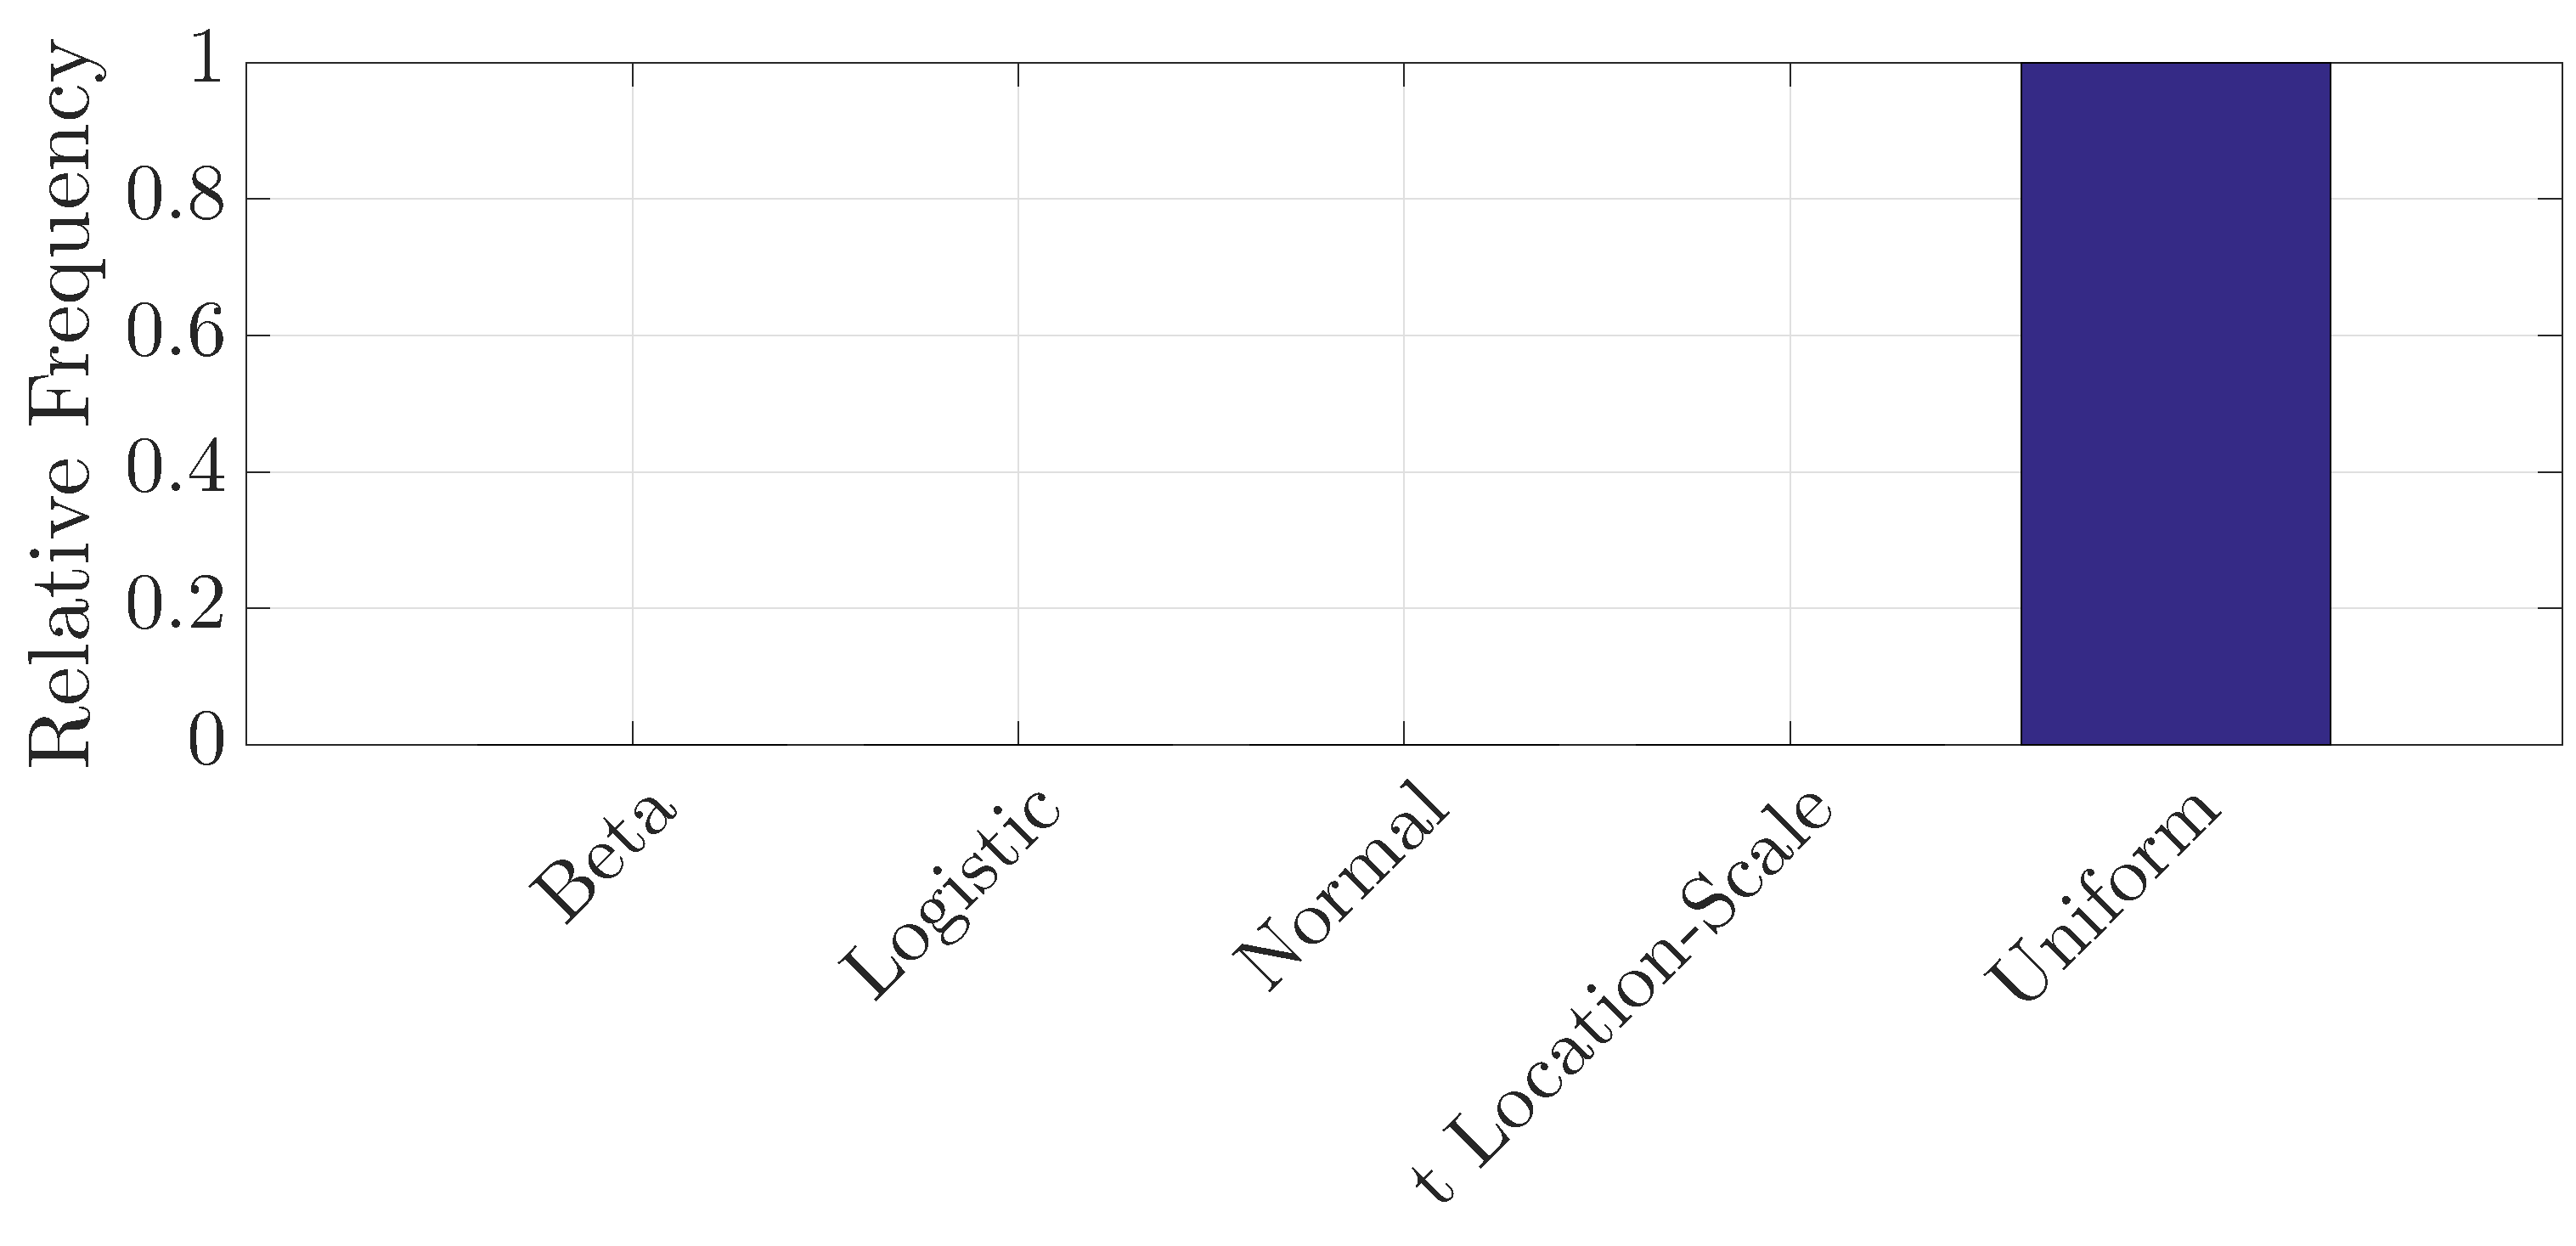
\includegraphics[width=0.9\textwidth]{images/Phase_percentsW.eps}
	\caption{The relative frequency associated with the chosen statistical distribution that best models CFR phase in accord with the adopted criteria.}
	\label{Phase_percentsW}
\end{figure}

\begin{figure}[h!]
	\centering
	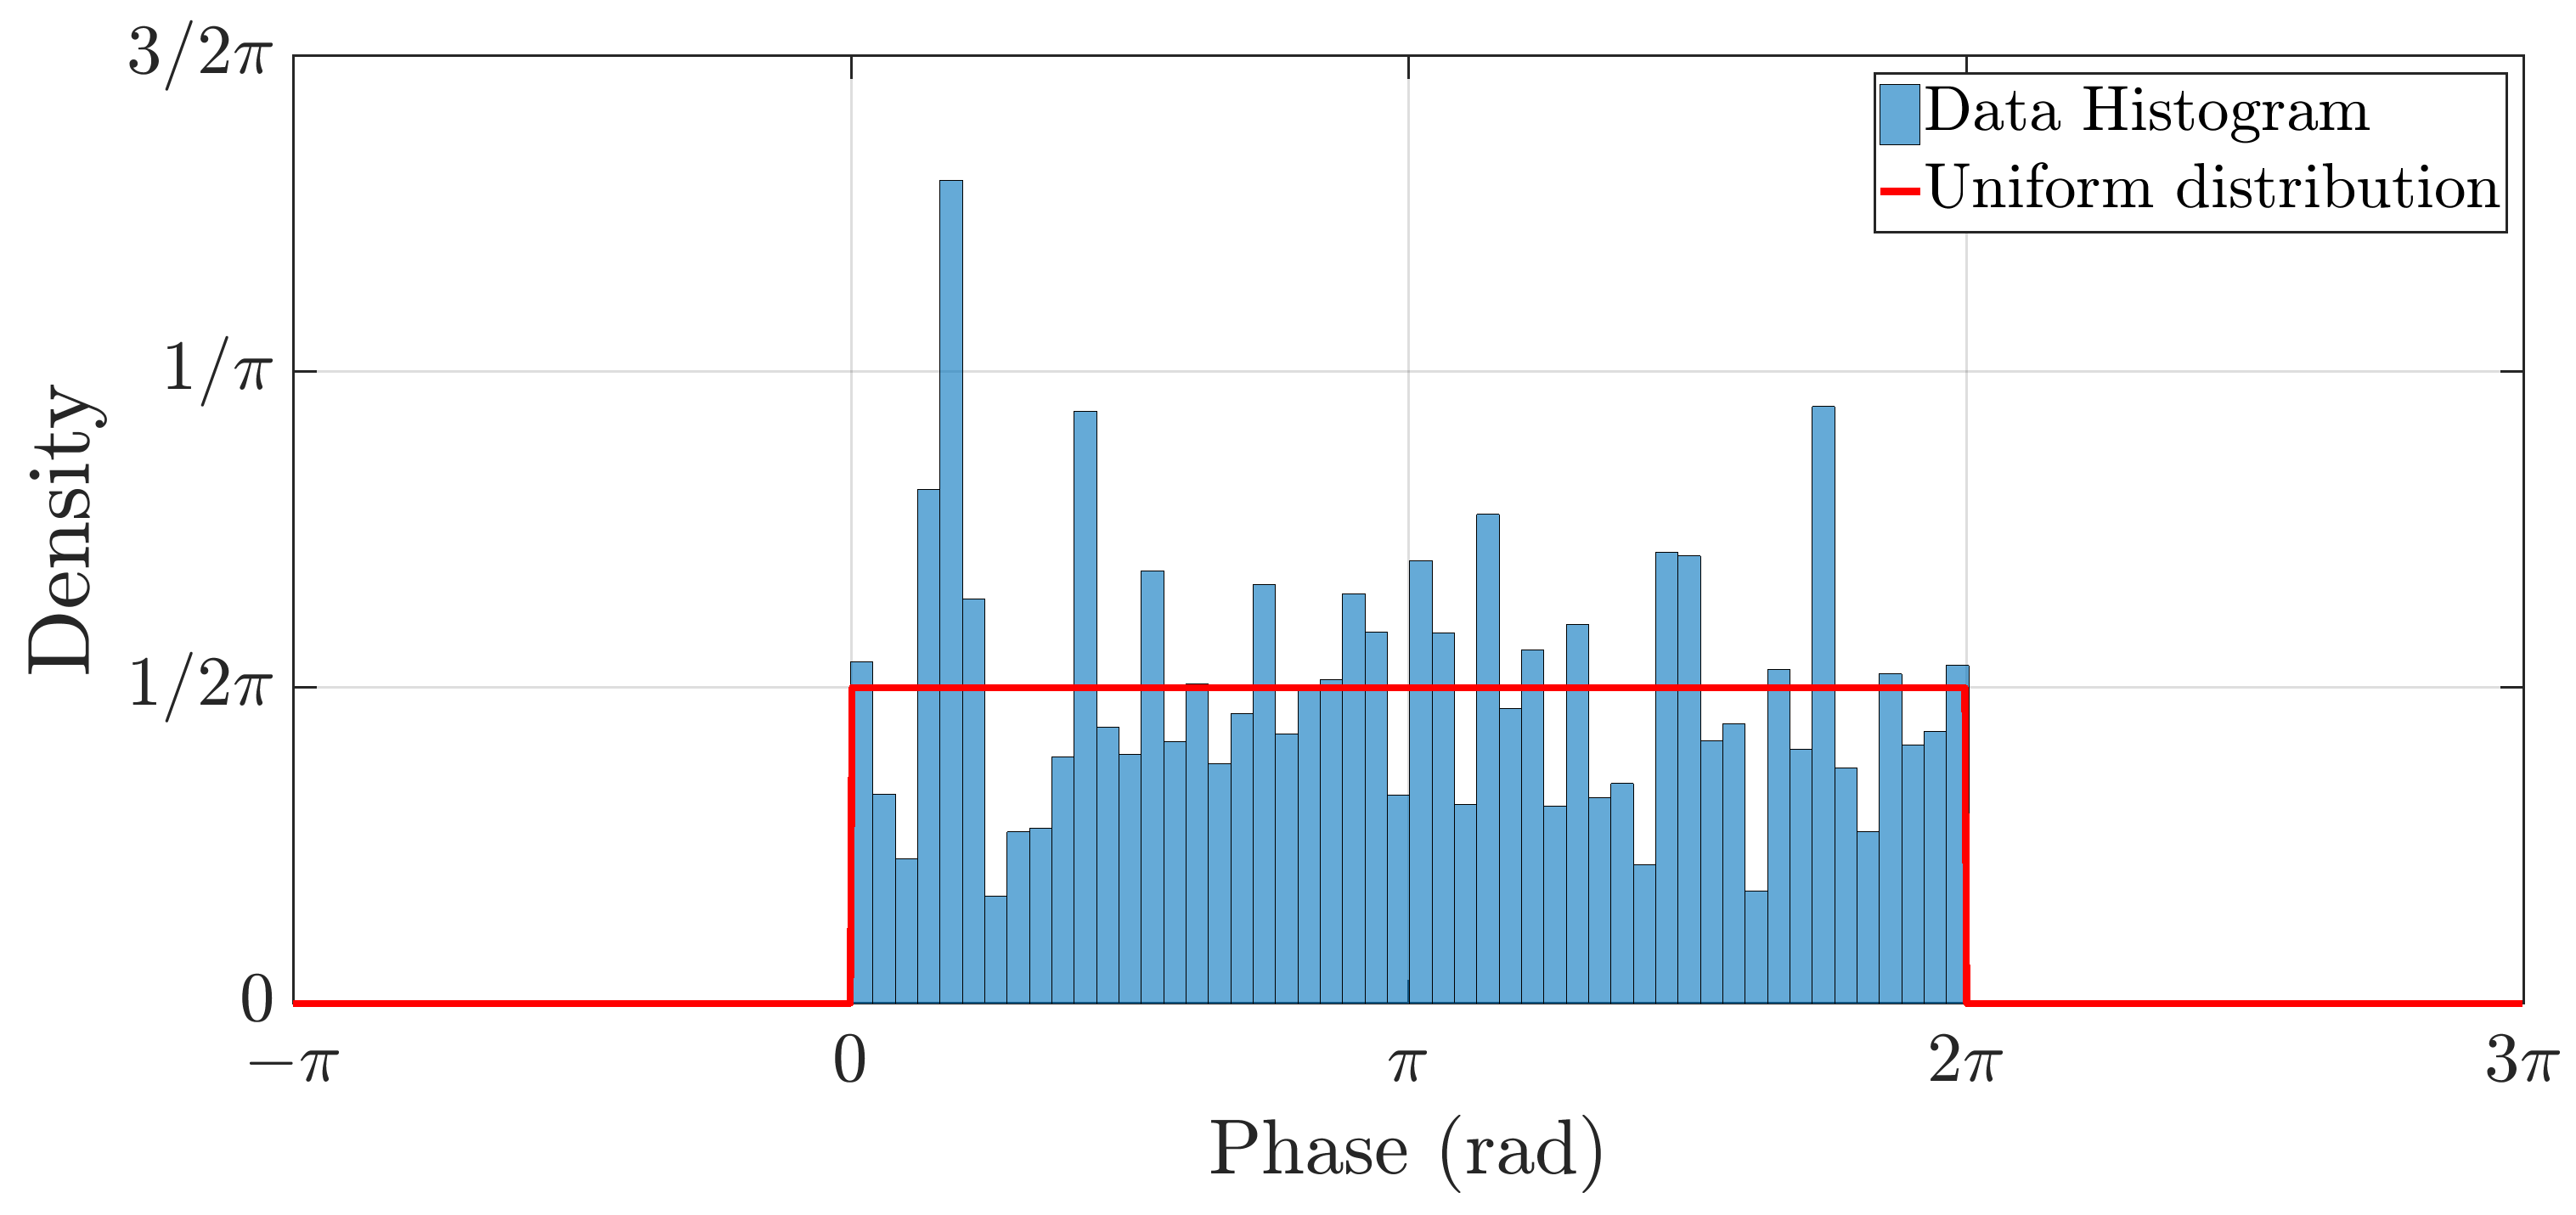
\includegraphics[width=0.9\textwidth]{images/Phase_histsW_2.eps}
	\caption{The relative frequency of the phase of the valid CFR estimates at the sample $k$ = 1040 ($k\Delta f= 50.78$ MHz) using the Uniform distribution.}
	\label{phase_examplesW}
\end{figure}

\begin{figure}[h!]
	\centering
	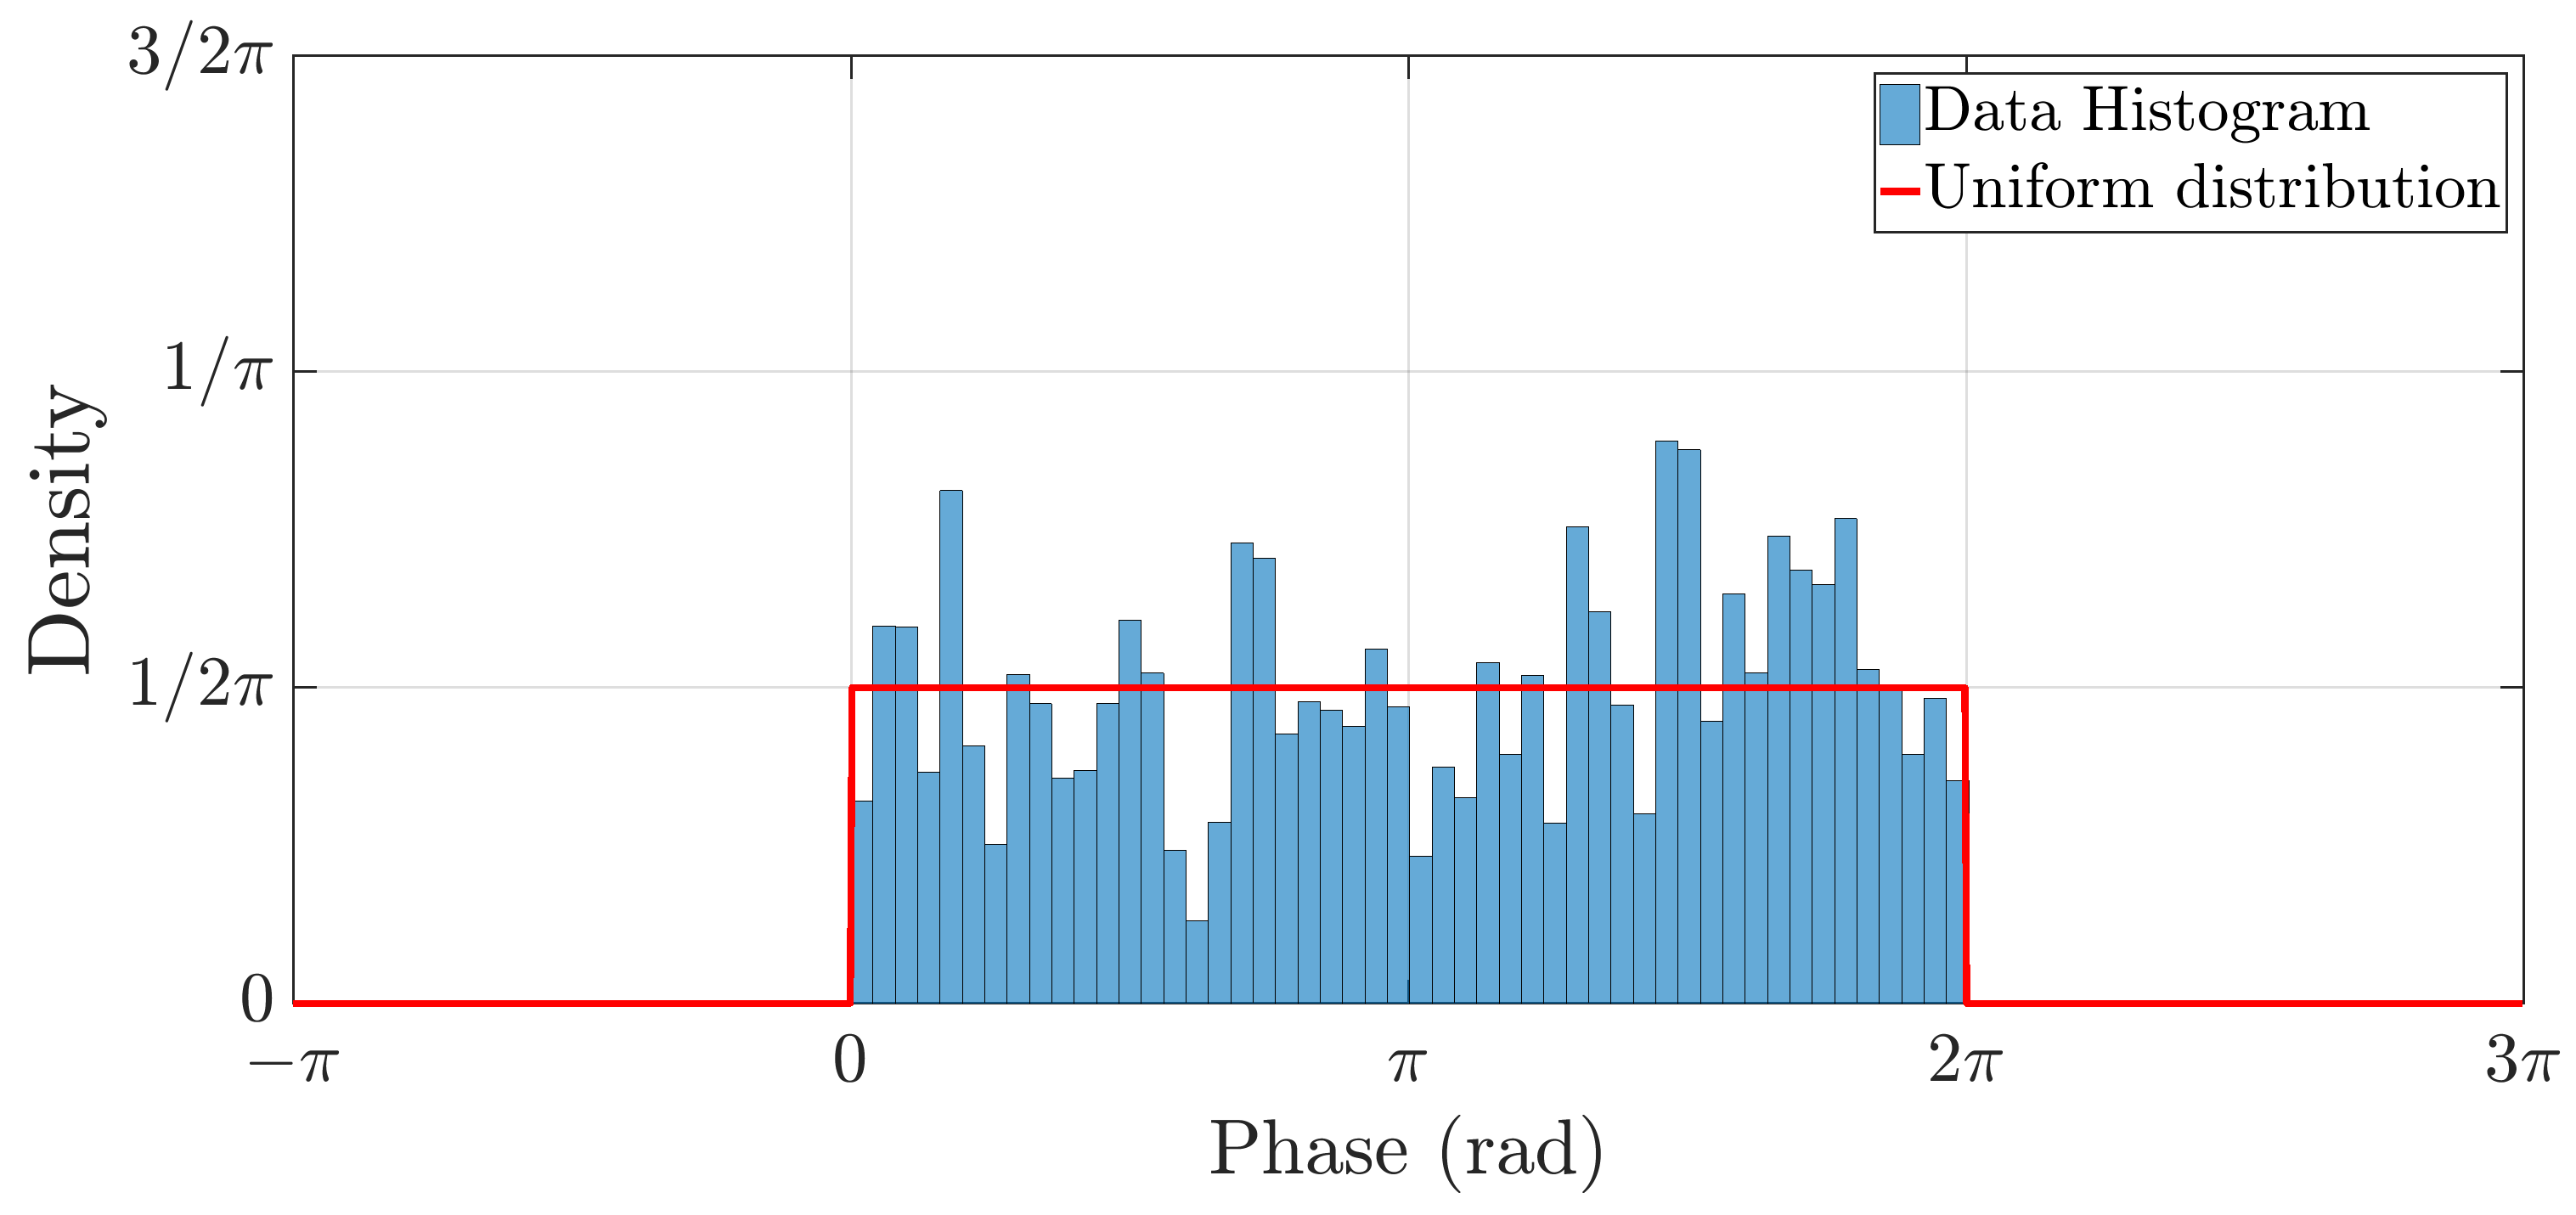
\includegraphics[width=0.9\textwidth]{images/Phase_hist2sW_2.eps}
	\caption{The relative frequency of the phase of the valid CFR estimates at the sample $k$ = 1650 ($k\Delta f= 80.57$ MHz) using the Uniform distribution.}
	\label{phase_example2sW}
\end{figure}

In a nutshell, the use of the proposed enhanced statistical modeling method for modeling the \ac{CFR} of in-home hybrid \ac{PLC}-\ac{WLC} \textit{short-path} channels showed that the magnitude component of them is a nonstationary random process, that can be modeled by the Log-normal distribution. The statistical analyses has also verified that, similarly to the \ac{PLC} channel, the phase component of in-home hybrid \ac{PLC}-\ac{WLC} \textit{short-path} channels can be modeled by the Uniform distribution with fixed parameters as frequency varies, thus denoting that the phase function of \ac{CFR} of in-home hybrid \ac{PLC}-\ac{WLC} \textit{short-path} channels is a stationary random process.

%%%%%%%%%%%%%%%%%%%%%%%%%%%%%%%%%%%%%%%%%%%%%%%%%%%%%%%%%%%%%%%%%%%%%%%
\section{UNCORRELATED CFR MODEL OF HYBRID PLC-WLC \textit{LONG-PATH} CHANNELS} \label{sec:NR4}
%%%%%%%%%%%%%%%%%%%%%%%%%%%%%%%%%%%%%%%%%%%%%%%%%%%%%%%%%%%%%%%%%%%%%%%

This section highlights the modeling of the \acp{CFR} data set related to \ac{PLC}-\ac{WLC} \textit{long-path} channels, which were acquired through the measurement campaign described in \cite{thiago:hyb}. Fig. \ref{respfreqlW} shows $5$ valid and consecutive estimates of the \ac{CFR} magnitude. On this scenario the average operation was not used on the \ac{CFR} estimates, since the coherence time of the \ac{PLC}-\ac{WLC} \textit{long-path} channels was not long enough to contain the duration of at least two symbol periods ($T_{sym}$). Note that the channel attenuation ranges from approximately $-45$~dB up to $15$~dB and that the plots cover a time interval equal to $\Delta T_{sym}\approx23.04\mu$s and, as a consequence, $5\Delta T = 115.2\mu$s.

\begin{figure}[h]
	\centering
	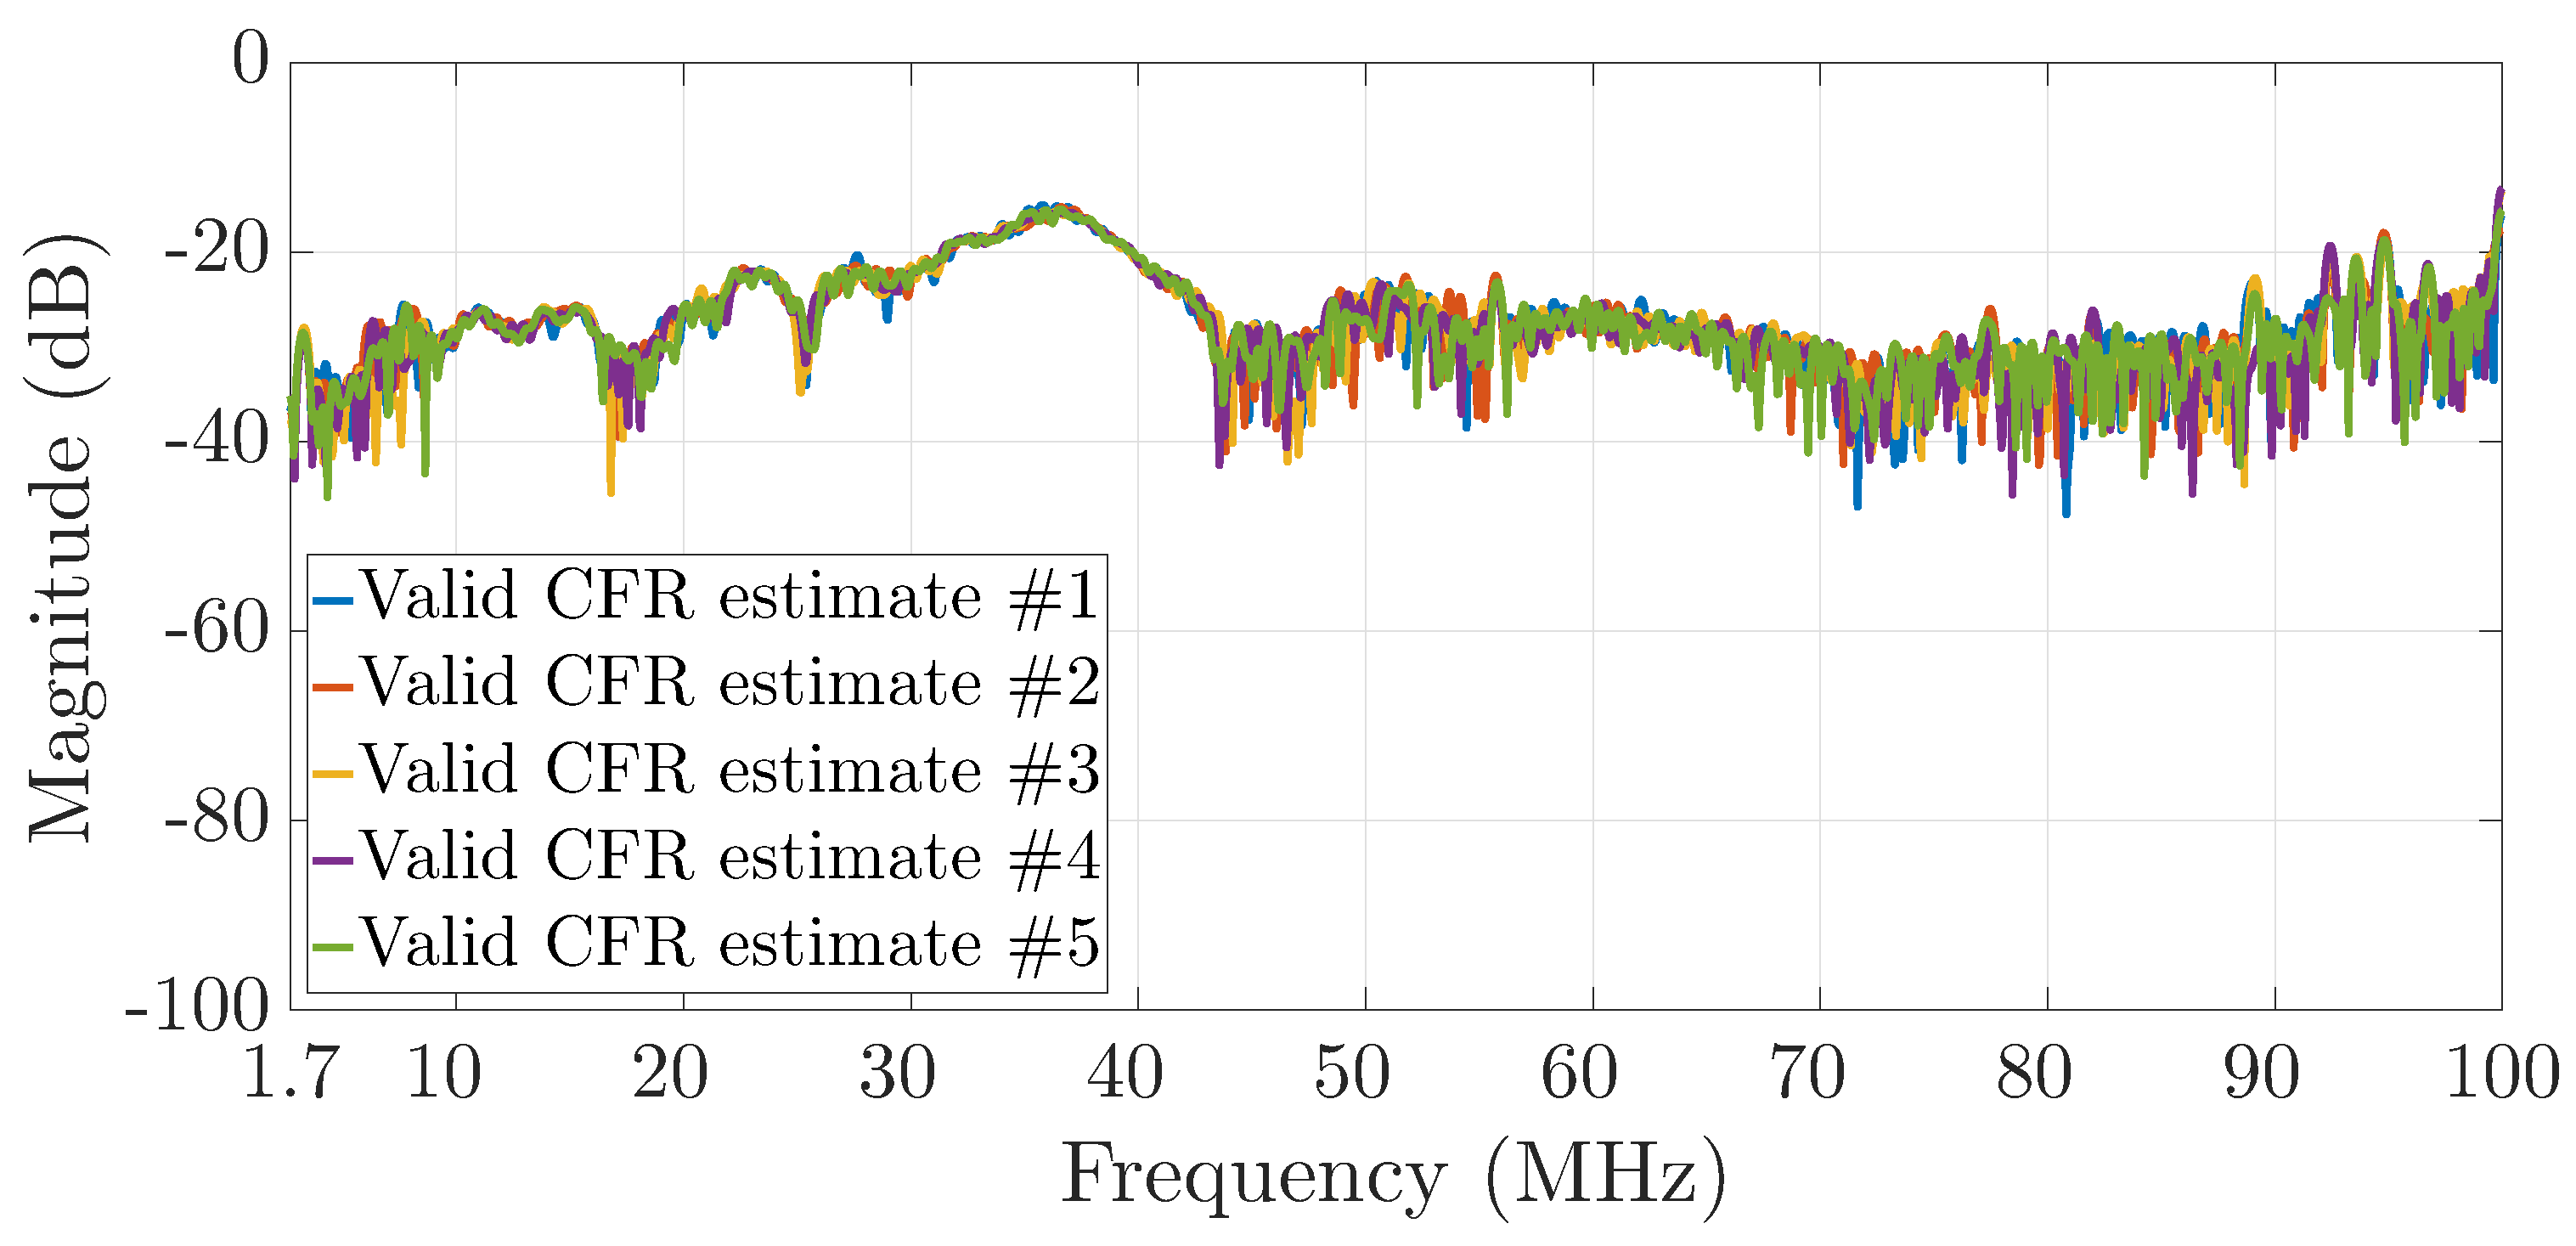
\includegraphics[width=0.9\textwidth]{images/respfreqlW.eps}
	\caption{Five consecutive and valid CFR magnitudes of the measured in-home PLC-WLC \textit{long-path} channel.}
	\label{respfreqlW}
\end{figure}

Fig. \ref{MAG_percentlW} illustrates the relative frequency of statistical distributions that had modeled, in accord with the adopted criteria, the magnitude of the whole set of valid \ac{CFR} estimates. Similarly to the results acquired on the \ac{PLC}-\ac{WLC} \textit{short-path} channels, a single statistical distribution have modeled the majority of the magnitudes, but another different statistical distribution stood out as possible candidate to model the \ac{CFR} magnitudes. As a matter of fact, in 51\% of the \ac{CFR} estimates the Log-normal distribution resulted in the best model and in 38\% of it the Gamma distribution offered the best modeling. 

\begin{figure}[h!]
	\centering
	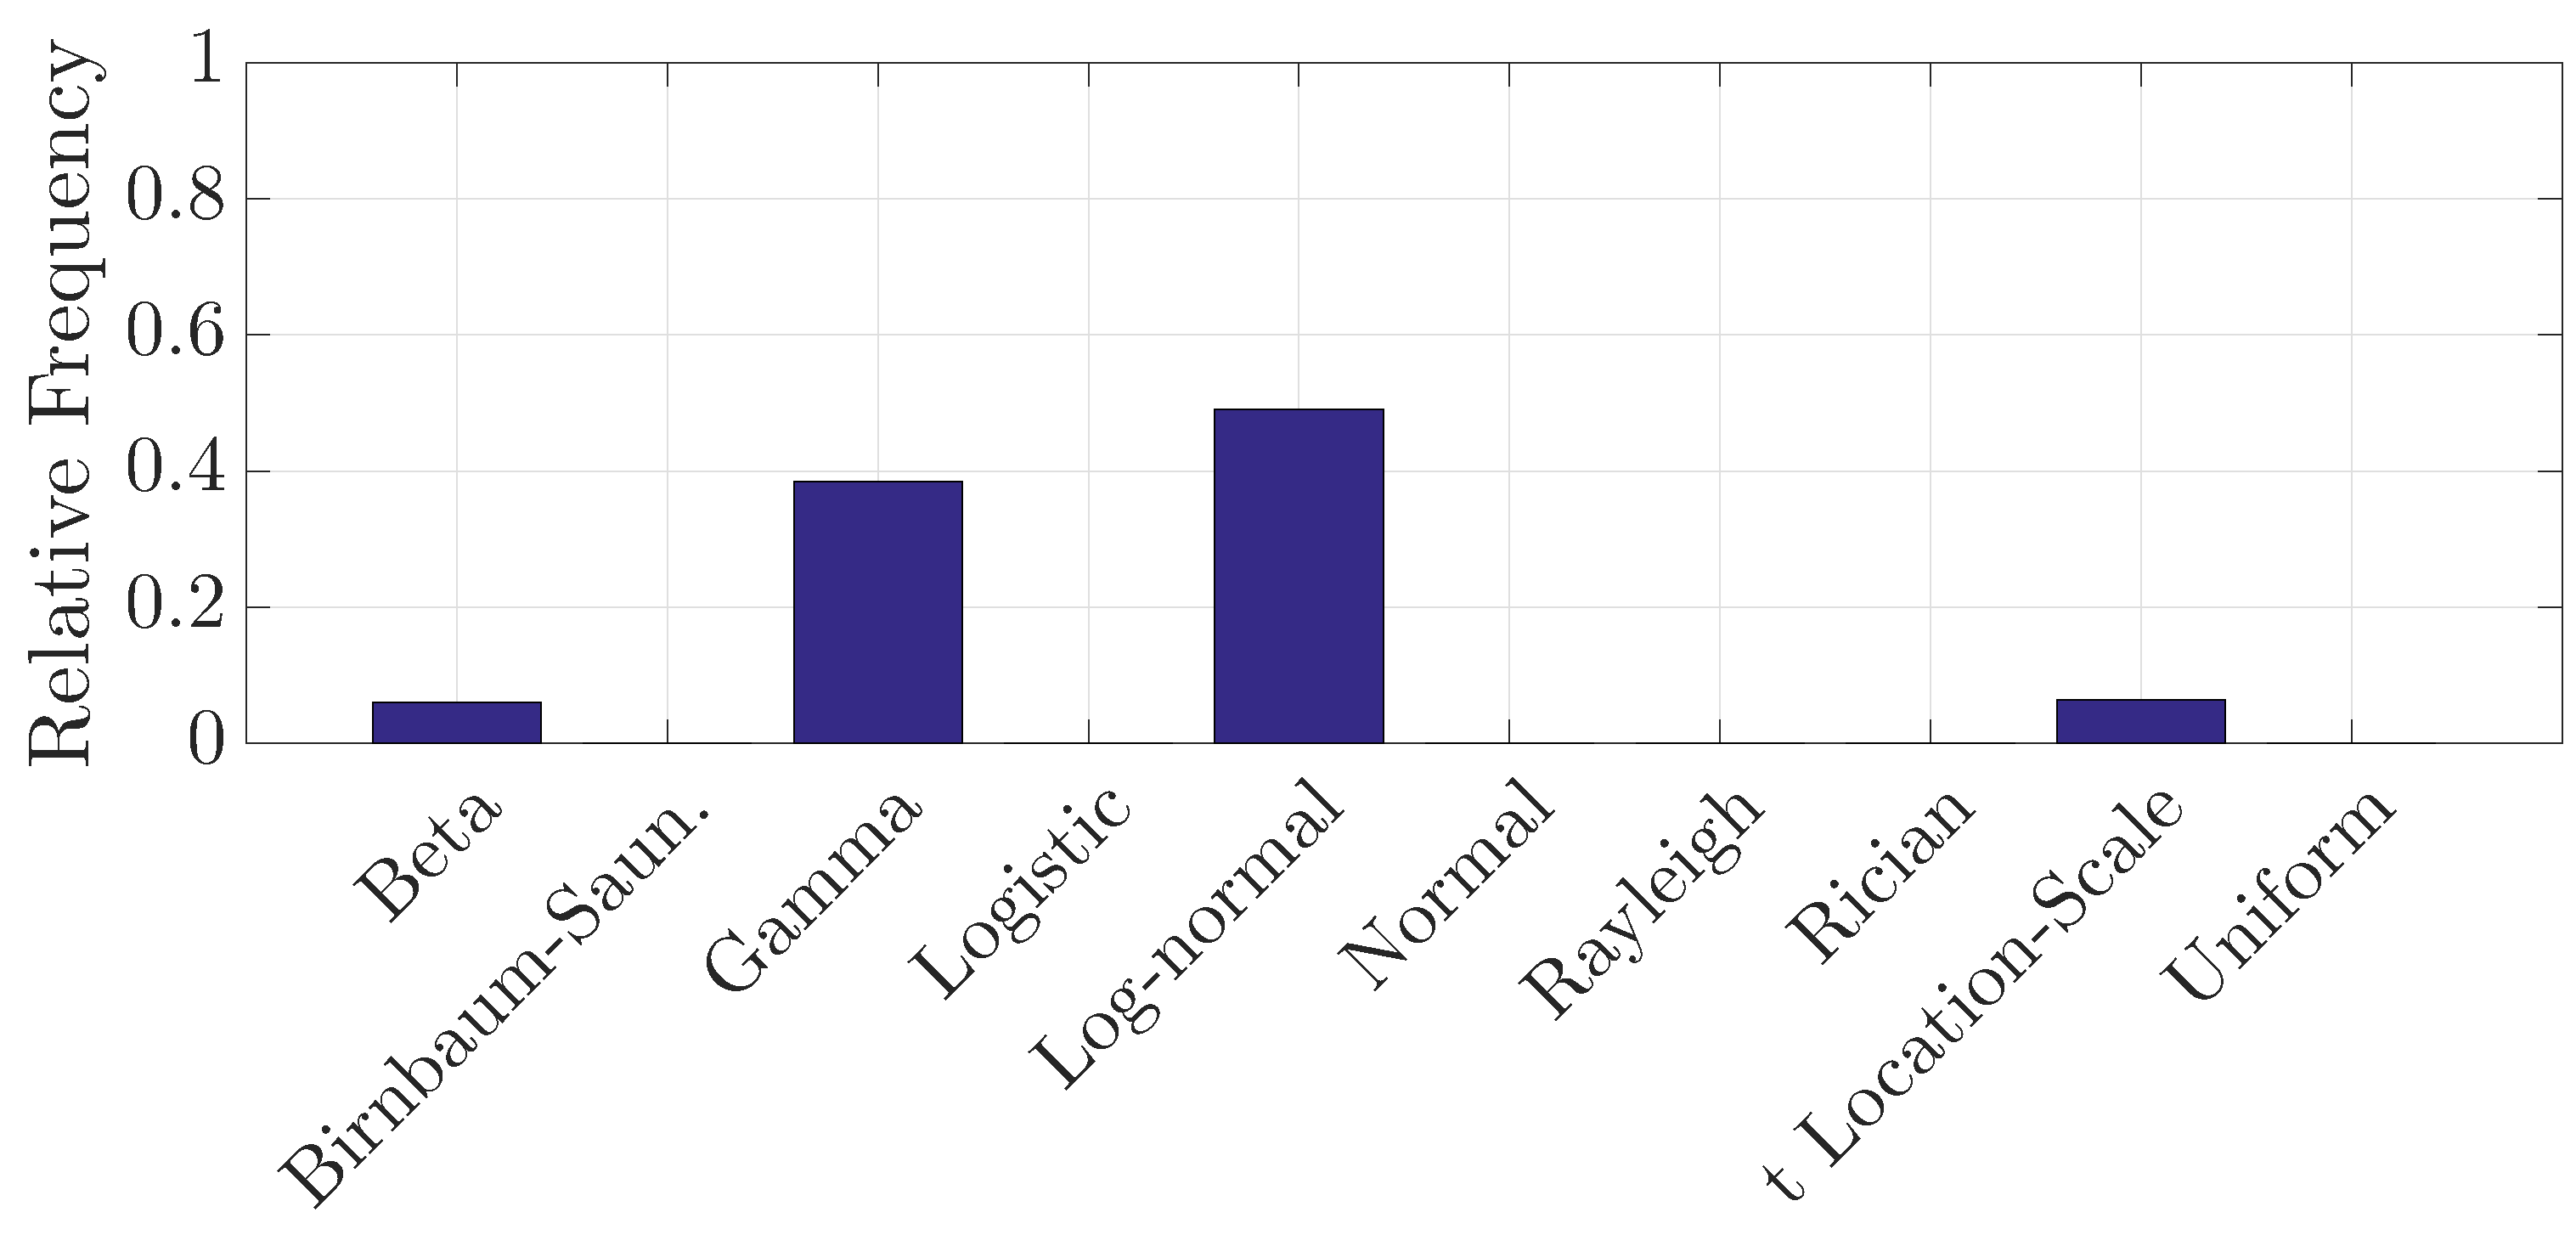
\includegraphics[width=0.9\textwidth]{images/Mag_percentlW.eps}
	\caption{The relative frequency associated with the chosen statistical distribution that best models the CFR magnitude in accord with the adopted criteria.}
	\label{MAG_percentlW}
\end{figure}

Once again the log-likelihood ratio $\rho_{MLE} (f)$ (\ref{eq:log-lik}) presented in the subsection \ref{sec:P1} was used in order to evaluate which of the two distributions is the best choice to model the magnitude component of the \ac{CFR} estimates. Fig. \ref{fig:Log_likelW} portrays the values of  $\rho_{MLE}(f)$ for the two best statistical distributions candidates to model the magnitude of the valid \ac{CFR} estimates. The threshold value of $1.2$ was again indicated as a red dashed line, under which the statistical distribution can be considered good enough to model the \ac{CFR}. These curves emphasize that only the Log-normal distributions achieved the minimum ratio over the \ac{MLE} criteria. Overall, the results presented in Fig. \ref{MAG_percentlW} and Fig. \ref{fig:Log_likelW} illustrates that the Log-normal distribution is the best option to model the magnitude of the valid \ac{CFR} estimates of the measured in-home hybrid \ac{PLC}-\ac{WLC} \textit{long-path} channels. In other words, the magnitude of the valid \ac{CFR} estimates of in-home hybrid \ac{PLC}-\ac{WLC} \textit{long-path} channels can be modeled by using only one statistical distribution (i.e., the Log-normal distribution).

%\begin{figure}[h!]
%	\centering
%	\psfrag{AAA}[c][c][1.3]{$\rho_{MLE} (f)$}
%	\subfloat[]{\includegraphics[width=0.9\textwidth]{images/Log_LogNlW.eps}}\\~\\
%	\psfrag{AAA}[c][c][1.3]{$\rho_{MLE} (f)$}
%	\subfloat[]{\includegraphics[width=0.9\textwidth]{images/Log_GammalW.eps}}\\~\\
%	\caption{The log-likelihood ratio for the following statistical distributions: (a) Log-normal, (b) Gamma.}
%	\label{fig:Log_likelW}
%\end{figure}

\begin{figure}[h!]
	\centering
	\psfrag{AAA}[c][c][1.3]{$\rho_{MLE} (f)$}
	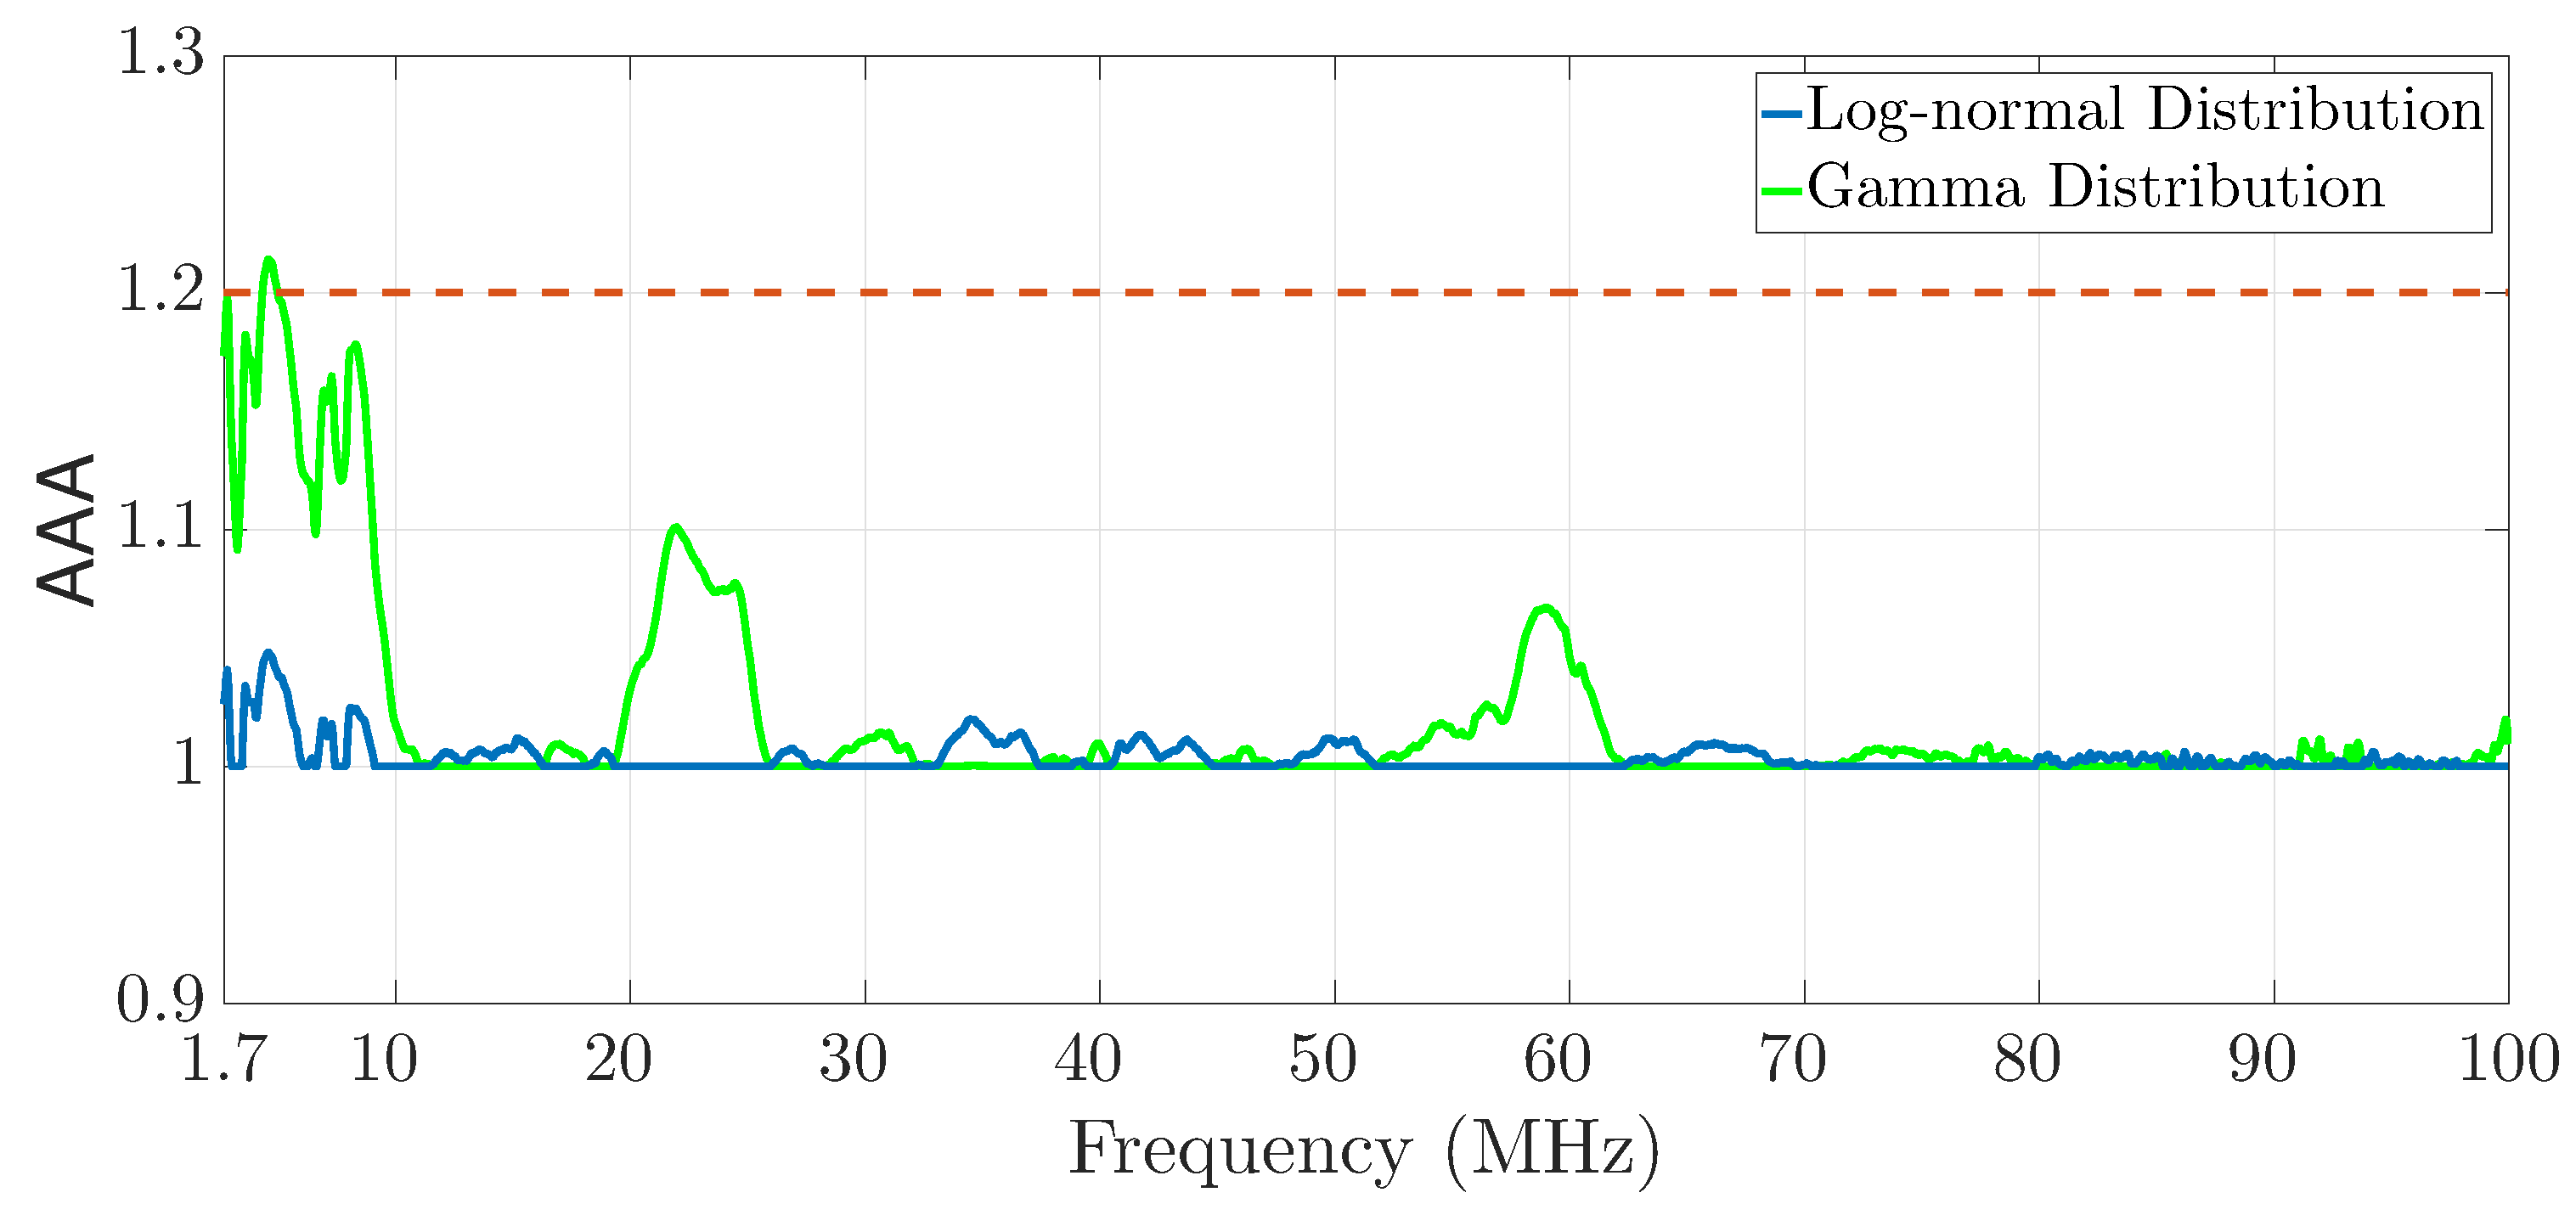
\includegraphics[width=0.9\textwidth]{images/Log_Lognormal_GammalW.eps}
	\caption{The log-likelihood ratio for the following statistical distributions: Log-normal, Gamma.}
	\label{fig:Log_likelW}
\end{figure}


The statistical analysis of the magnitude of the valid \ac{CFR} estimates shows that the parameters of the Log-normal distribution assume different values as frequency changes. If $\mathcal{C}_{k} = \{\zeta_1[k],\zeta_2[k]\}$ is the set of parameters for the statistical distribution modeling the magnitude of the valid \ac{CFR} estimates of \ac{PLC}-\ac{WLC} \textit{short-path} channels, where $k=0,1,\cdots,N-1$,  $\zeta_1[k] = \mu[k]$ and $\zeta_2[k] = \sigma[k]$, are the two parameters ($U=2$) of the Log-normal distribution, named mean and standard deviation respectively, associated with the $k$-th sample of the valid \ac{CFR}. Then, Fig. \ref{mag_examplelW} and Fig. \ref{mag_example2lW} illustrates the statistical models for two different values of frequency: $f=51.76$~MHz ($k=1060 \rightarrow f = 1060\Delta f$) and $f=78.1$~MHz ($k=1600 \rightarrow f = 1600\Delta f$), respectively. The parameters of the Log-normal distribution are  $\mu(1060 \Delta f) = \zeta_1[1060]=-6.0759$ and $\sigma( 1060 \Delta f) = \zeta_2[1040] = 0.8118$; $\mu(1600 \Delta f) = \zeta_1[1600] = -6.8347$ and $\sigma( 1600 \Delta f) = \zeta_2[1600]=0.8407$ for $f=51.76$~MHz and $f=78.1$~MHz, respectively.

\begin{figure}[h!]
	\centering
	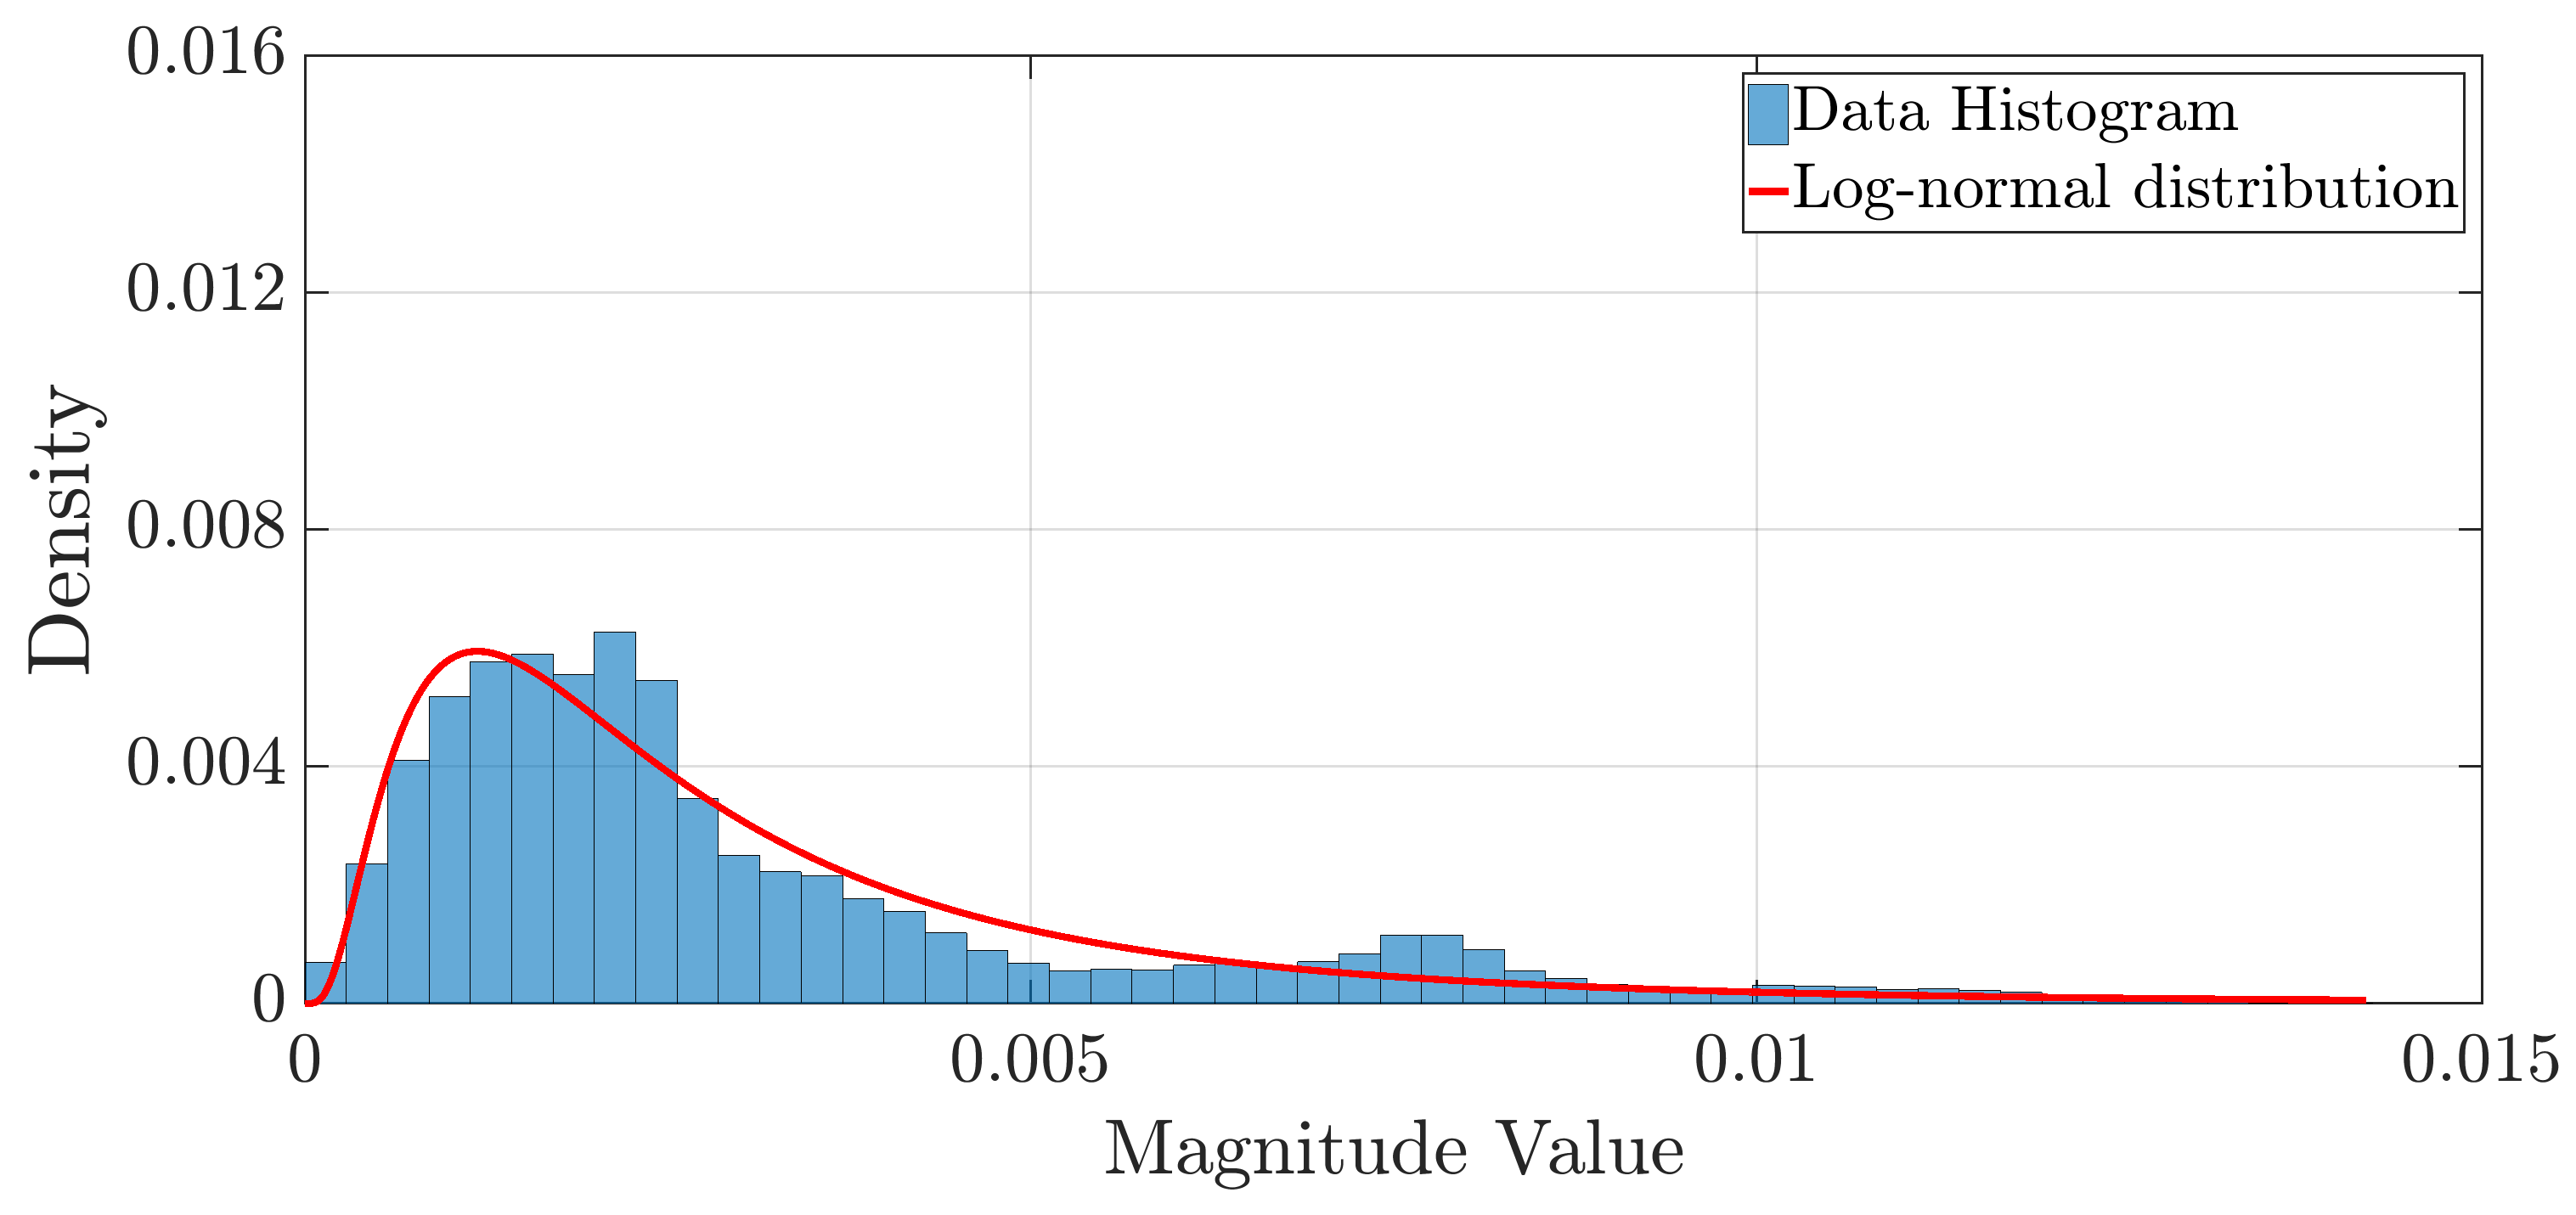
\includegraphics[width=0.9\textwidth]{images/Mag_histlW_2.eps}
	\caption{The relative frequency of the magnitude of the valid CFR estimates at the sample $k = 1060$ ($k\Delta f= 51.76$~MHz) and the modeling based on the Log-normal distribution.}
	\label{mag_examplelW}
\end{figure}

\begin{figure}[h!]
	\centering
	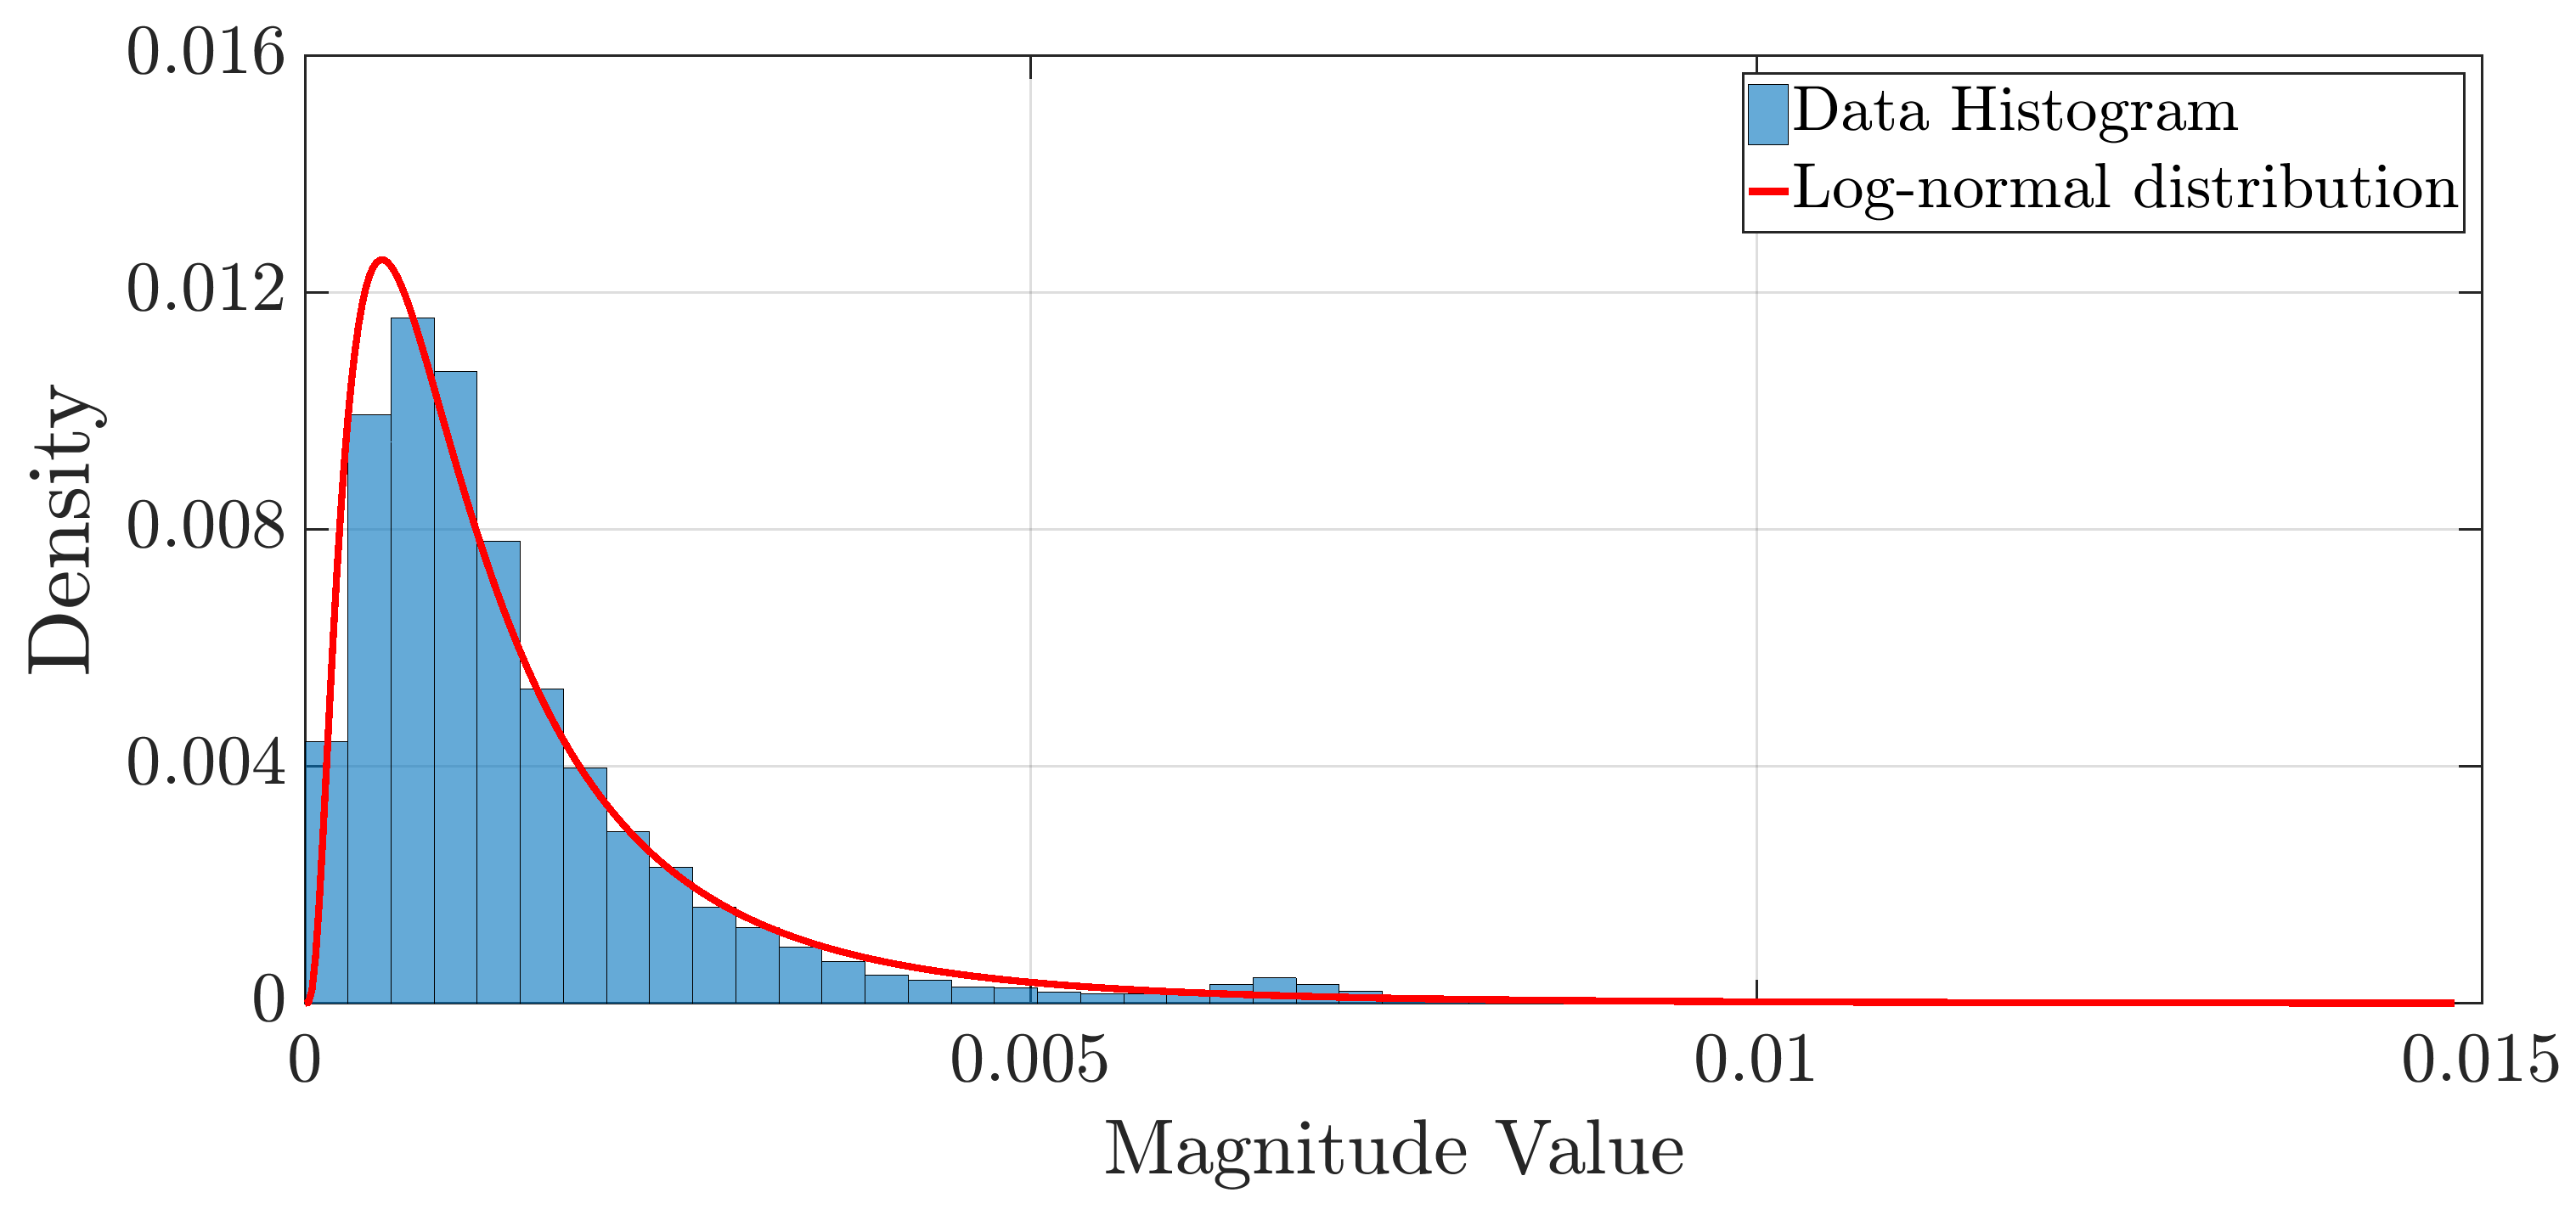
\includegraphics[width=0.9\textwidth]{images/Mag_hist2lW_2.eps}
	\caption{ The relative frequency of the magnitude of the valid CFR estimates at the sample $k = 1600$ ($k\Delta f= 78.1$~MHz) and the modeling based on the Log-normal distribution.}
	\label{mag_example2lW}
\end{figure}

Fig. \ref{fig:boundsLW} portrays the \ac{MSE} results in terms of the number of subbands for the in-home \ac{PLC}-\ac{WLC} \textit{long-path} channels. According to this plot, independent of the chosen criterion to select the non-uniformity of the subbands, the \ac{MSE} value does not change significantly as the number of subbands becomes higher than $15$. Due to a trade off between the precision of the interpolation and complexity of computing it, $L=15$ was chosen as the number of subbands. By interpolating the parameters values $\mu(k\Delta f)$ and $\sigma(k\Delta f)$ of the Log-normal distributions associated with the model of \ac{PLC}-\ac{WLC} \textit{long-path} \ac{CFR} using $L=15$ subbands and the Algorithm \ref{Algo2}, the continuous curves of parameters $\hat{\mu}(\omega)$ and $\hat{\sigma}(\omega)$ are yielded. Finally, the curves $\hat{\mu}(f)$ and $\hat{\sigma}(f)$ are easily obtained because $\omega \in [0,\pi)$ directly corresponds to the frequency band between $0$ and $100$~MHz. Figs. \ref{Fit_alfalW} and \ref{Fit_betalW} shows the curves for the parameters $\mu(f)$ and $\sigma(f)$, which are obtained by applying frequency domain interpolation technique detailed in \cite{mitra} and the curves obtained by using the cubic Spline interpolation with $L=15$ subbands. Furthermore, Table \ref{table_alfalW} (see Appendix \ref{ap:g}) lists the cubic Spline coefficients for modeling the parameter $\mu(f)$, of the valid \ac{CFR} magnitude. Similarly, Table \ref{table_betalW} (see Appendix \ref{ap:g}) lists the cubic Spline coefficients for modeling the parameter $\sigma(f)$. As a result, the coefficients values, the waveforms  $\hat{\mu(f)}$ and $\hat{\sigma(f)}$, and the Log-normal distribution define the random process representing the magnitude of the \ac{CFR} of the in-home \ac{PLC}-\ac{WLC} \textit{long-path} channel.

\begin{figure}[h!]
	\centering
	\subfloat[]{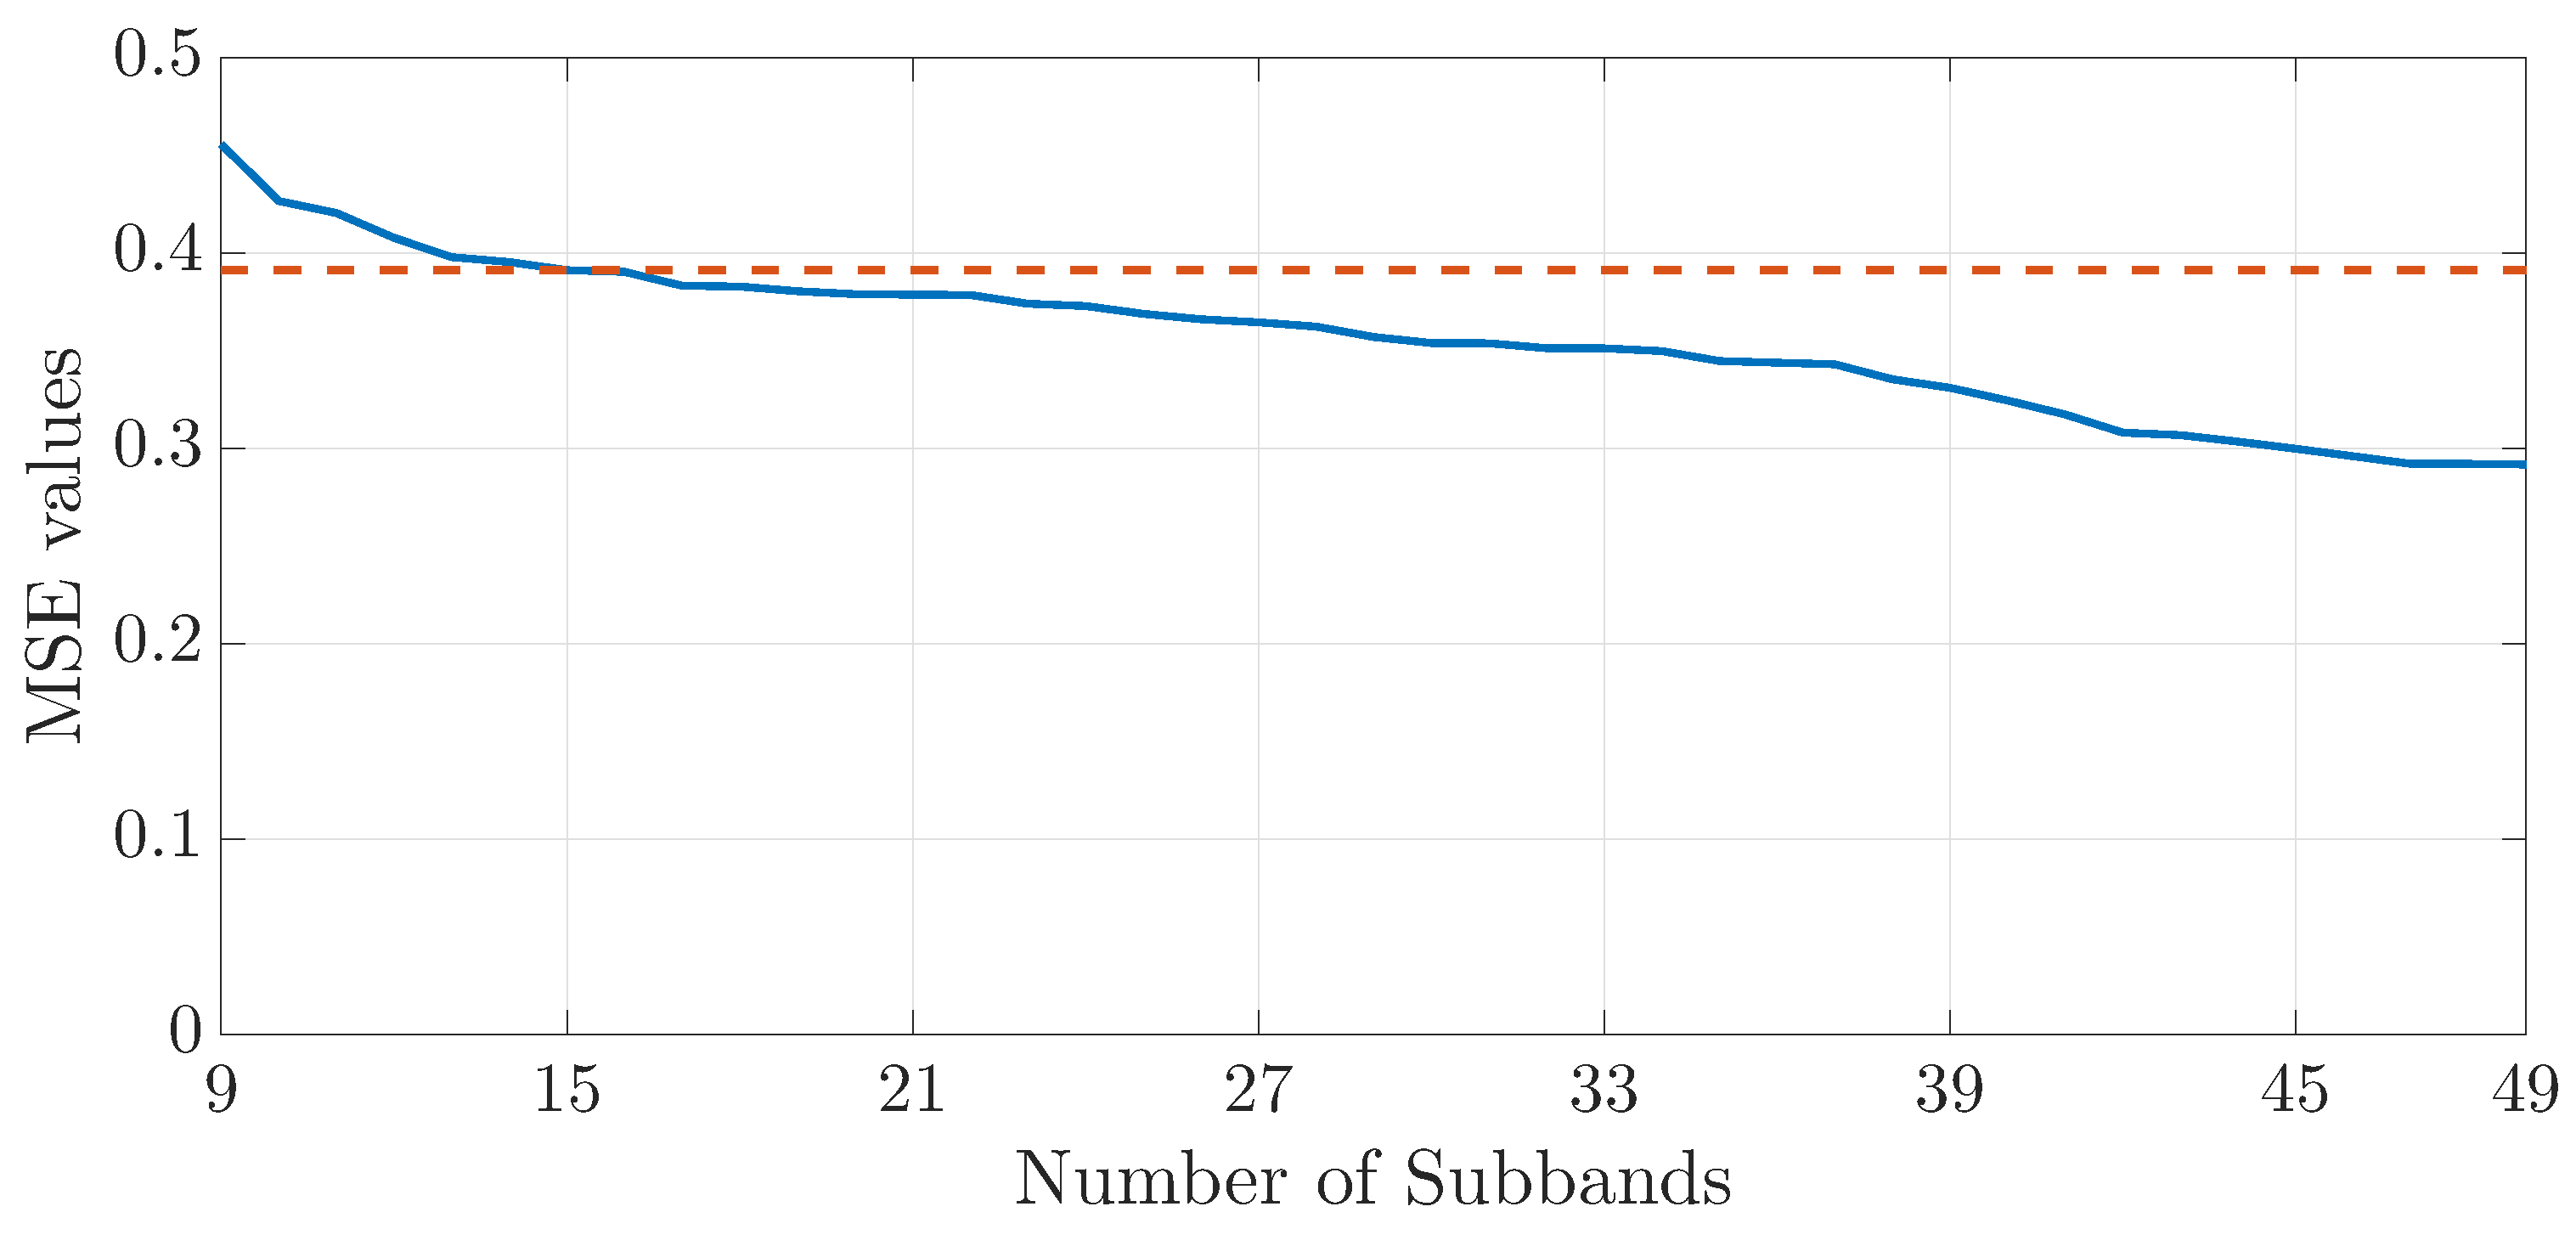
\includegraphics[width=0.9\textwidth]{images/alfalW_bounds.eps}}\\~\\
	\subfloat[]{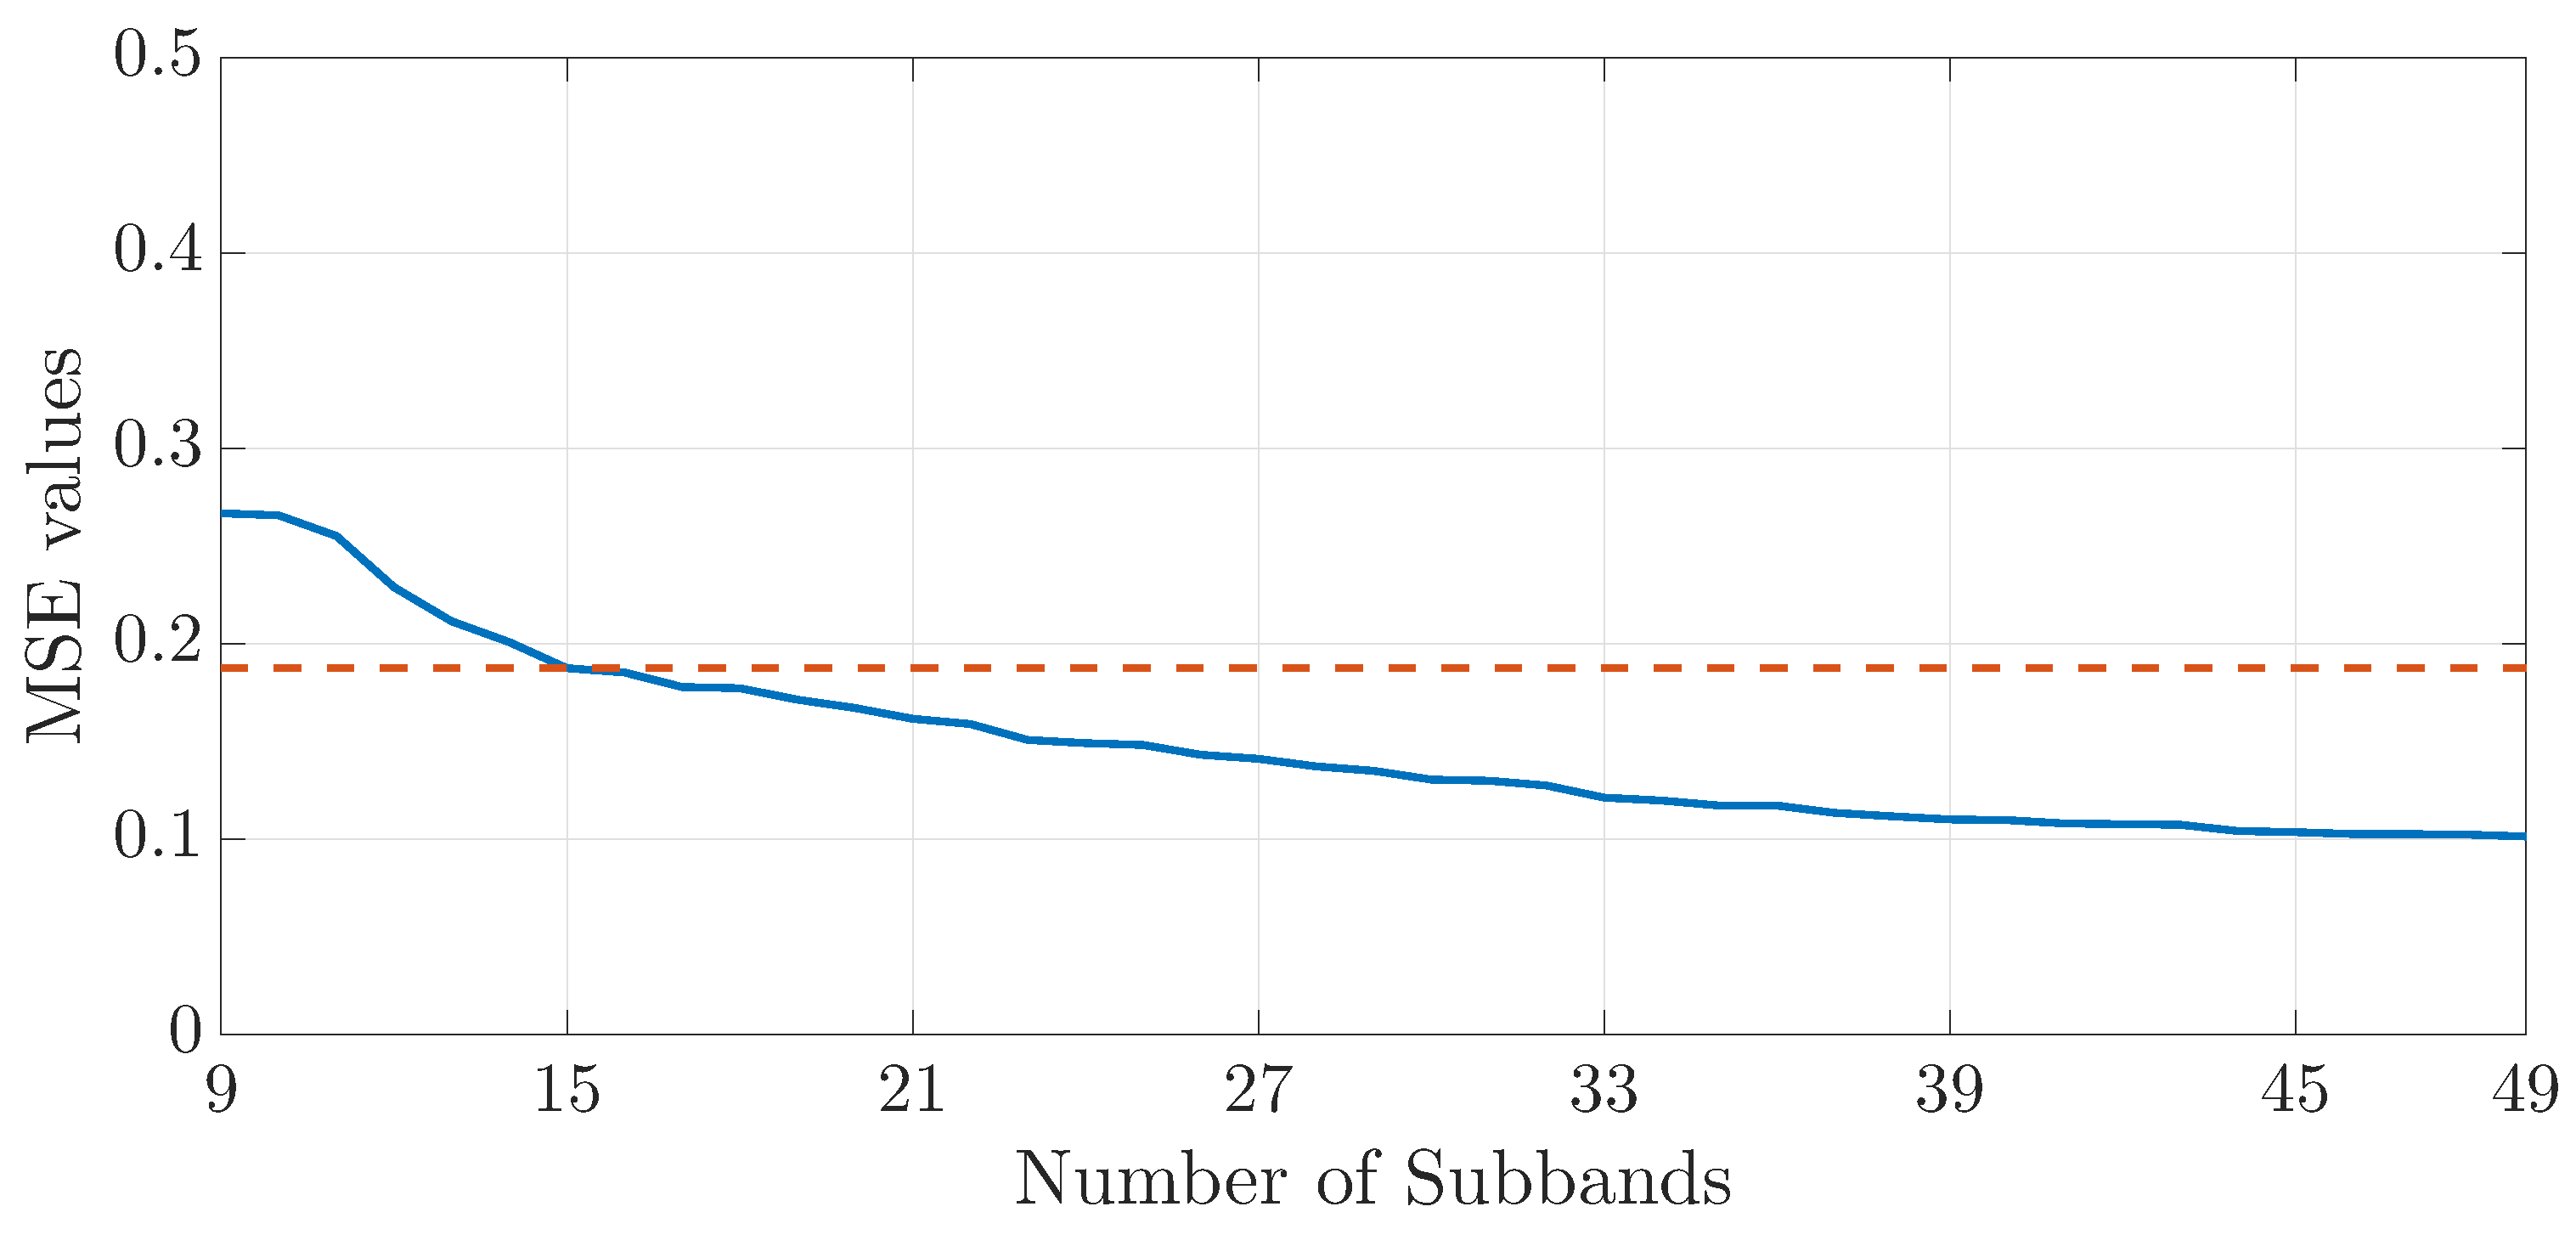
\includegraphics[width=0.9\textwidth]{images/betalW_bounds.eps}}\\~\\
	\caption{The MSE values for the parameters from PLC-WLC \textit{long-path} scenario: (a) $\mu$ parameter, (b) $\sigma$ parameter.}
	\label{fig:boundsLW}
\end{figure}

\begin{figure}[h]
	\centering
	\psfrag{Interval Boundsaa}[c][c][1]{Interval Bounds}
	\psfrag{AAA}[c][c][1]{$~~~~~\mu(k \Delta f)$}
	\psfrag{BBB}[c][c][1]{$~\hat{\mu}(f)$}
	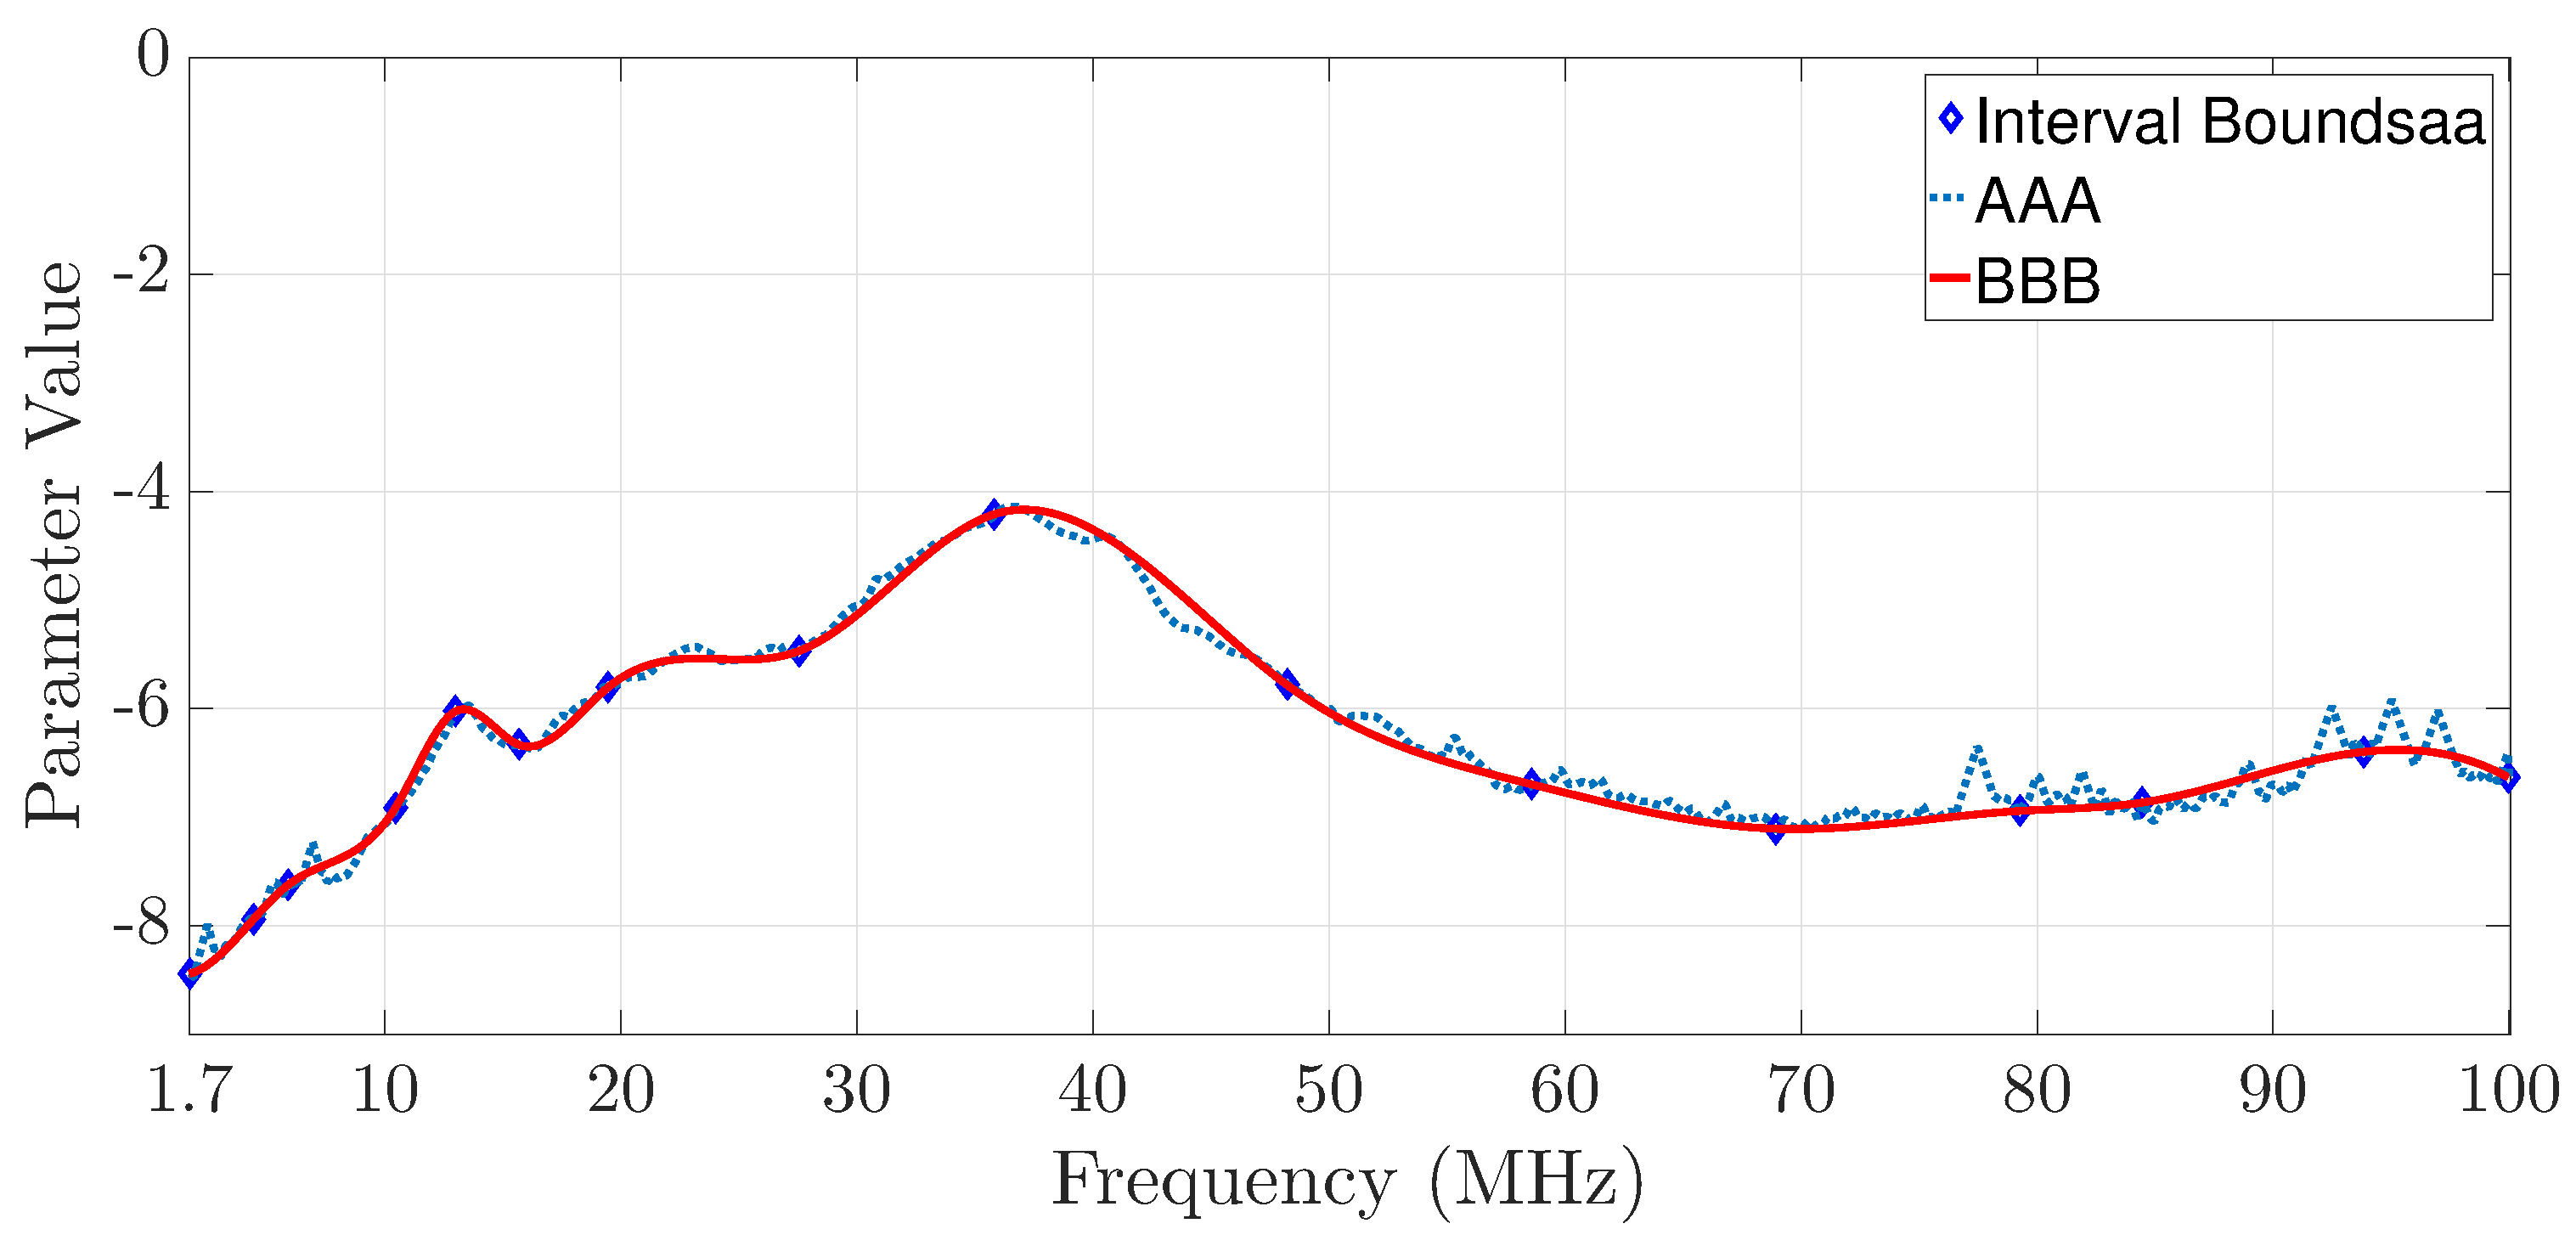
\includegraphics[width=0.92\textwidth]{images/Alfa_fitlW.eps}
	\caption{The result of the interpolation technique based on cubic Splines applied to obtain $\mu(f)=\zeta_1(f)$ for the Log-normal distribution (${\mu}(k \Delta f)$ are the original values of the parameter and $\hat{\mu}(f)$ is the interpolated curve).}
	\label{Fit_alfalW}
\end{figure}

\begin{figure}[h]
	\centering
	\psfrag{Interval Boundsaa}[c][c][1]{Interval Bounds}
	\psfrag{AAA}[c][c][1]{$~~~~~{\sigma}(k \Delta f)$}
	\psfrag{BBB}[c][c][1]{$~\hat{\sigma}(f)$}
	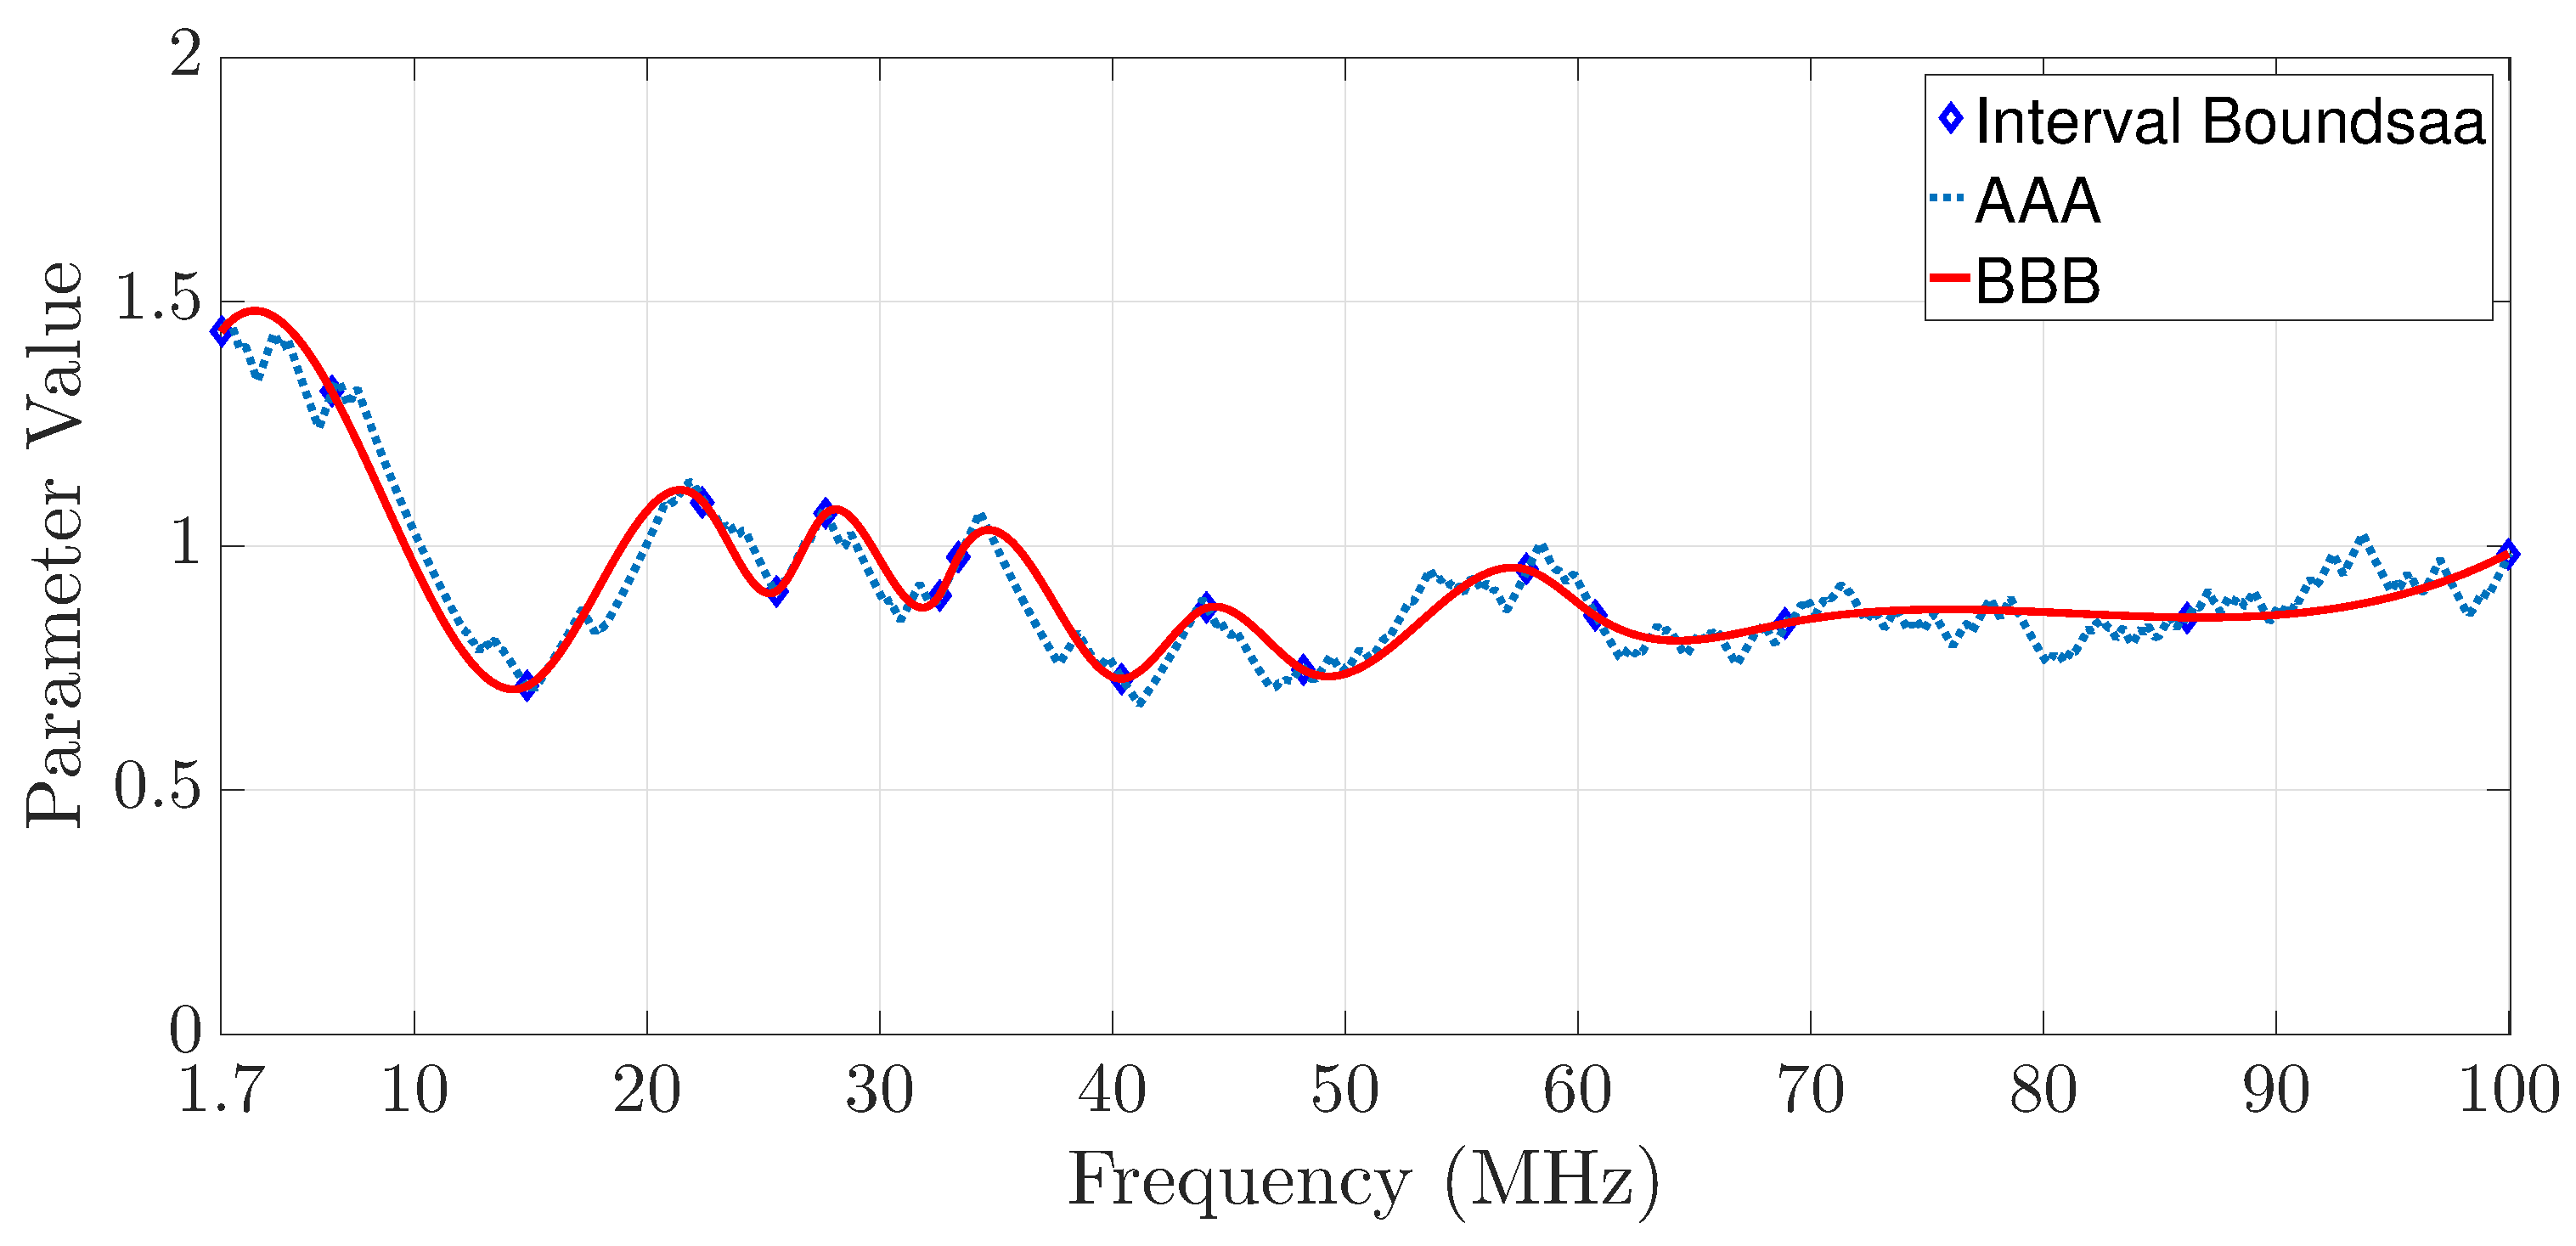
\includegraphics[width=0.9\textwidth]{images/Beta_fitlW.eps}
	\caption{The result of the interpolation technique based on cubic Splines applied to obtain $\sigma(f)=\zeta_2(f)$ for the Log-normal distribution (${\sigma}(k \Delta f)$ are the original values of the parameter and $\hat{\sigma}(f)$ is the interpolated curve).}
	\label{Fit_betalW}
\end{figure}

Fig. \ref{Phase_percentlW} shows the relative frequency of statistical distributions that had modeled, in accord with the adopted criteria, the phase of the whole set of valid \ac{CFR} estimates. Note that 100\% of the data set is best modeled by the Uniform distribution. On this scenario, differently form the statistical modeling of the \ac{CFR} magnitude, the statistical modeling of the phase of the valid \ac{CFR} estimates shows that each sample of it can be modeled by the same set of parameters of the Uniform distribution. In other words, $\Theta_k \in [0, 2\pi]$ denotes the interval of values that the phase of the valid \ac{CFR} estimates can assume and it defines the support for the Uniform distribution. 

Fig. \ref{phase_examplelW} and Fig. \ref{phase_example2lW} illustrates the statistical models regarding the frequencies $f=51.76$~MHz ($k=1060 \rightarrow f = 1060\Delta f$) and $f=78.1$~MHz ($k=1600 \rightarrow f = 1600\Delta f$), respectively. Independent of the frequency values, the phase model of the valid \ac{CFR} estimates remains the same. As a result, by using the Uniform distribution defined in the interval $[0, 2\pi]$, the random process representing the phase of the in-home \ac{PLC}-\ac{WLC} \textit{long-path} channel is yielded.

\begin{figure}[h!]
	\centering
	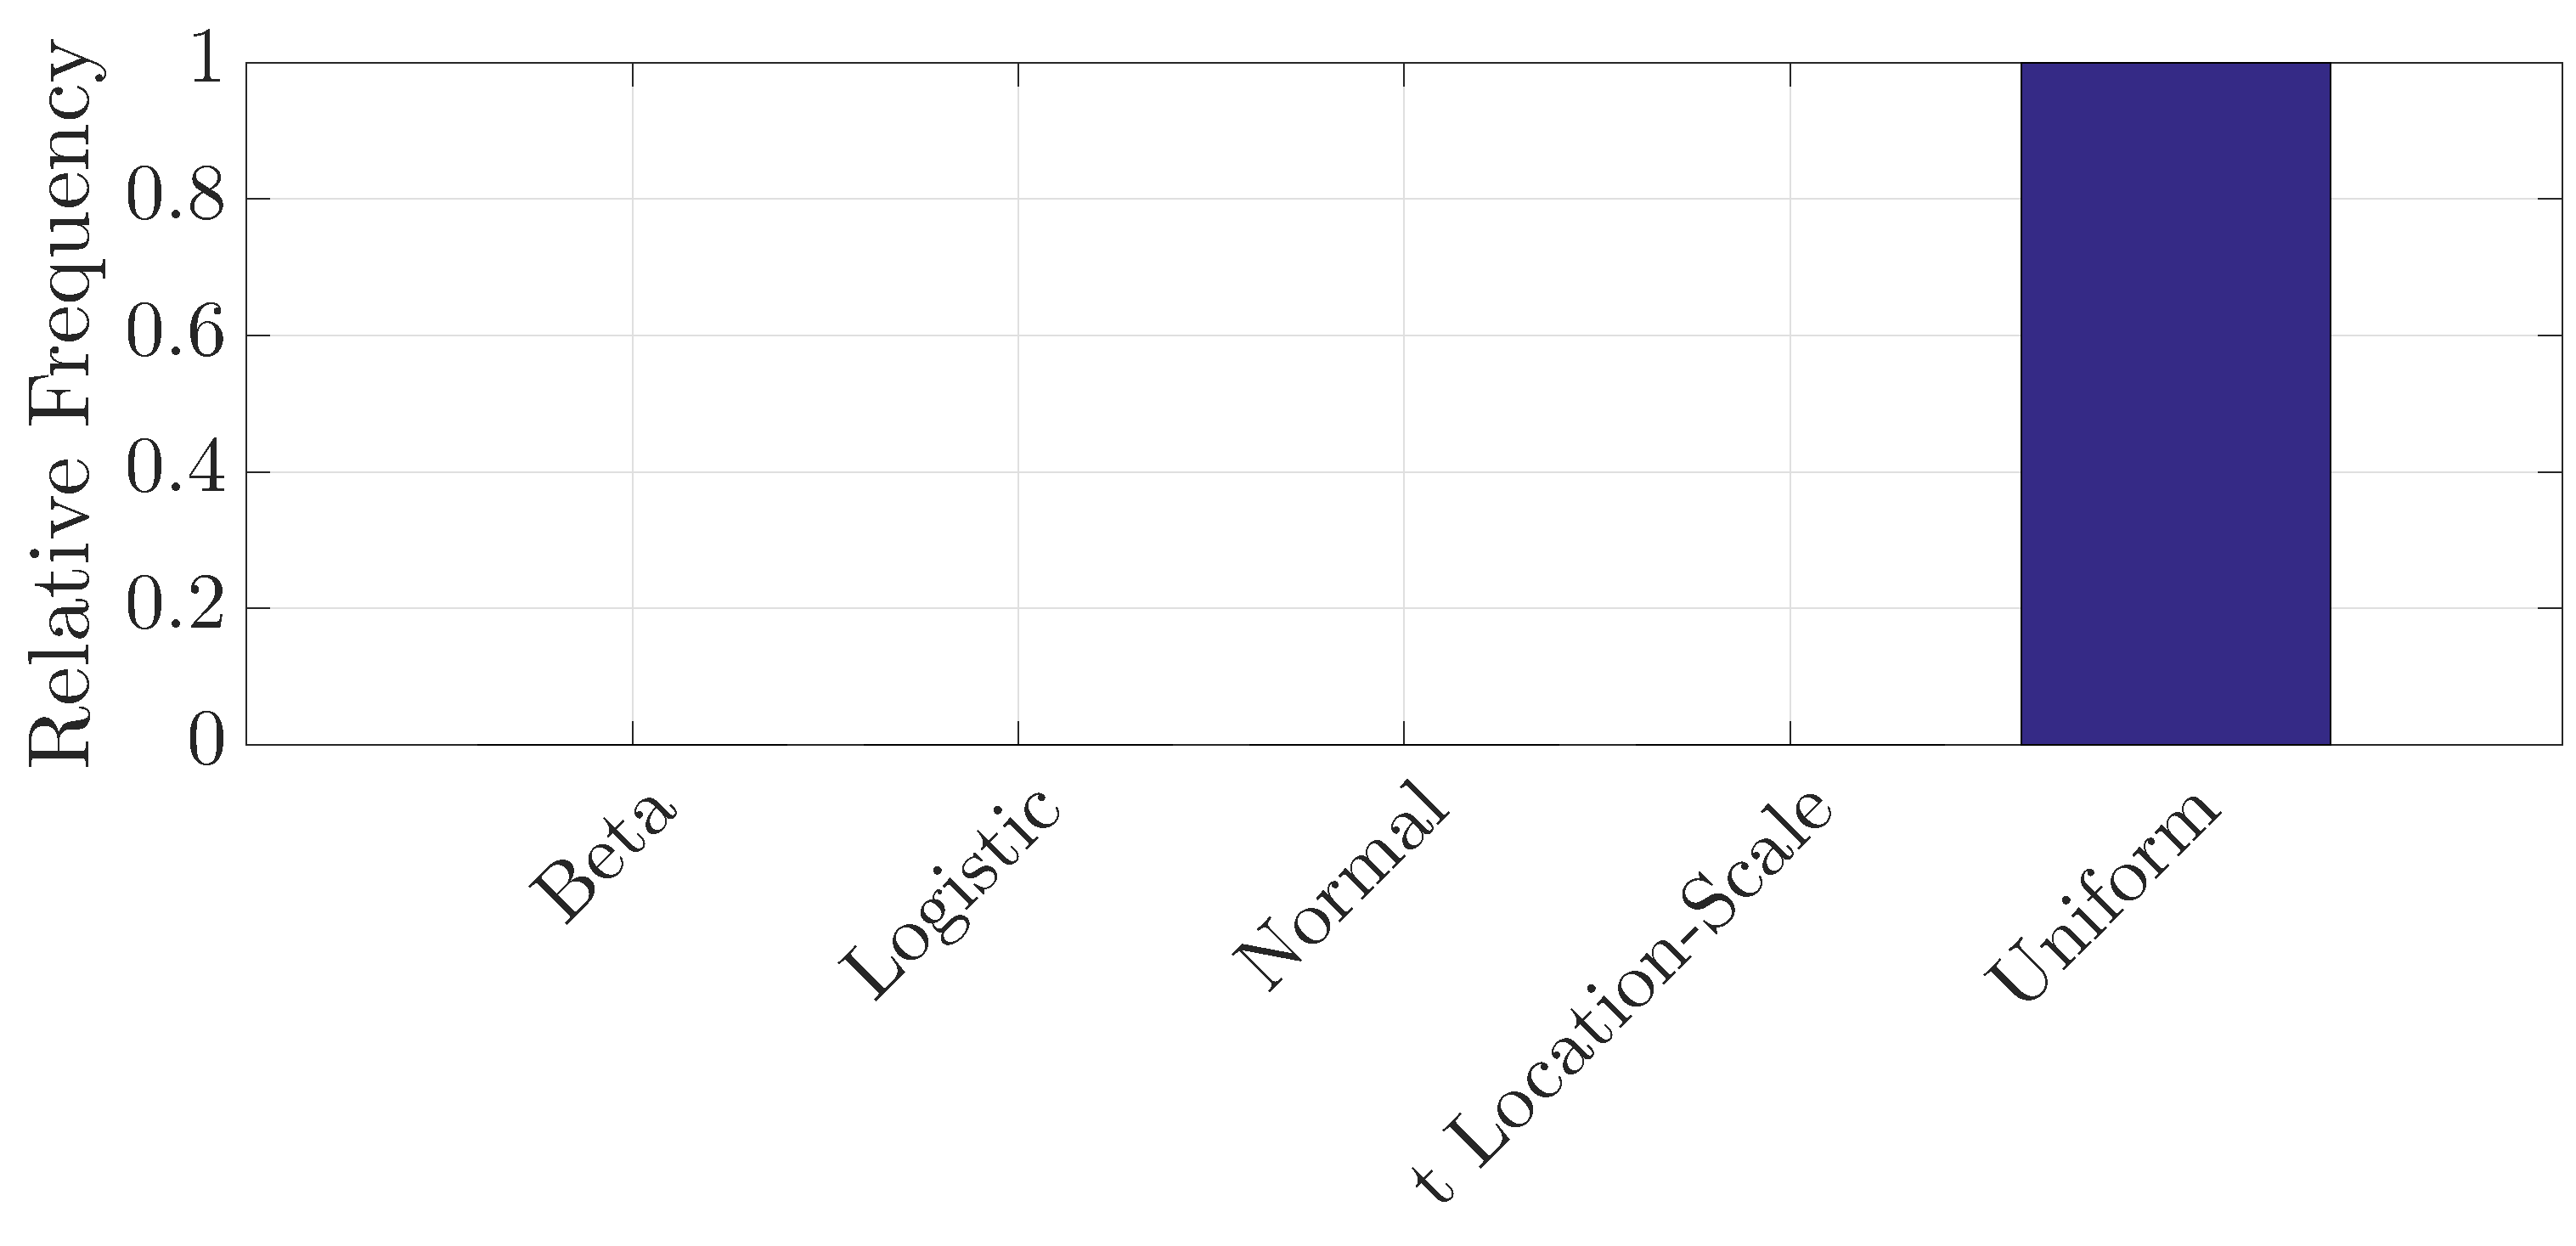
\includegraphics[width=0.9\textwidth]{images/Phase_percentlW.eps}
	\caption{The relative frequency associated with the chosen statistical distribution that best models CFR phase in accord with the adopted criteria.}
	\label{Phase_percentlW}
\end{figure}

\begin{figure}[h!]
	\centering
	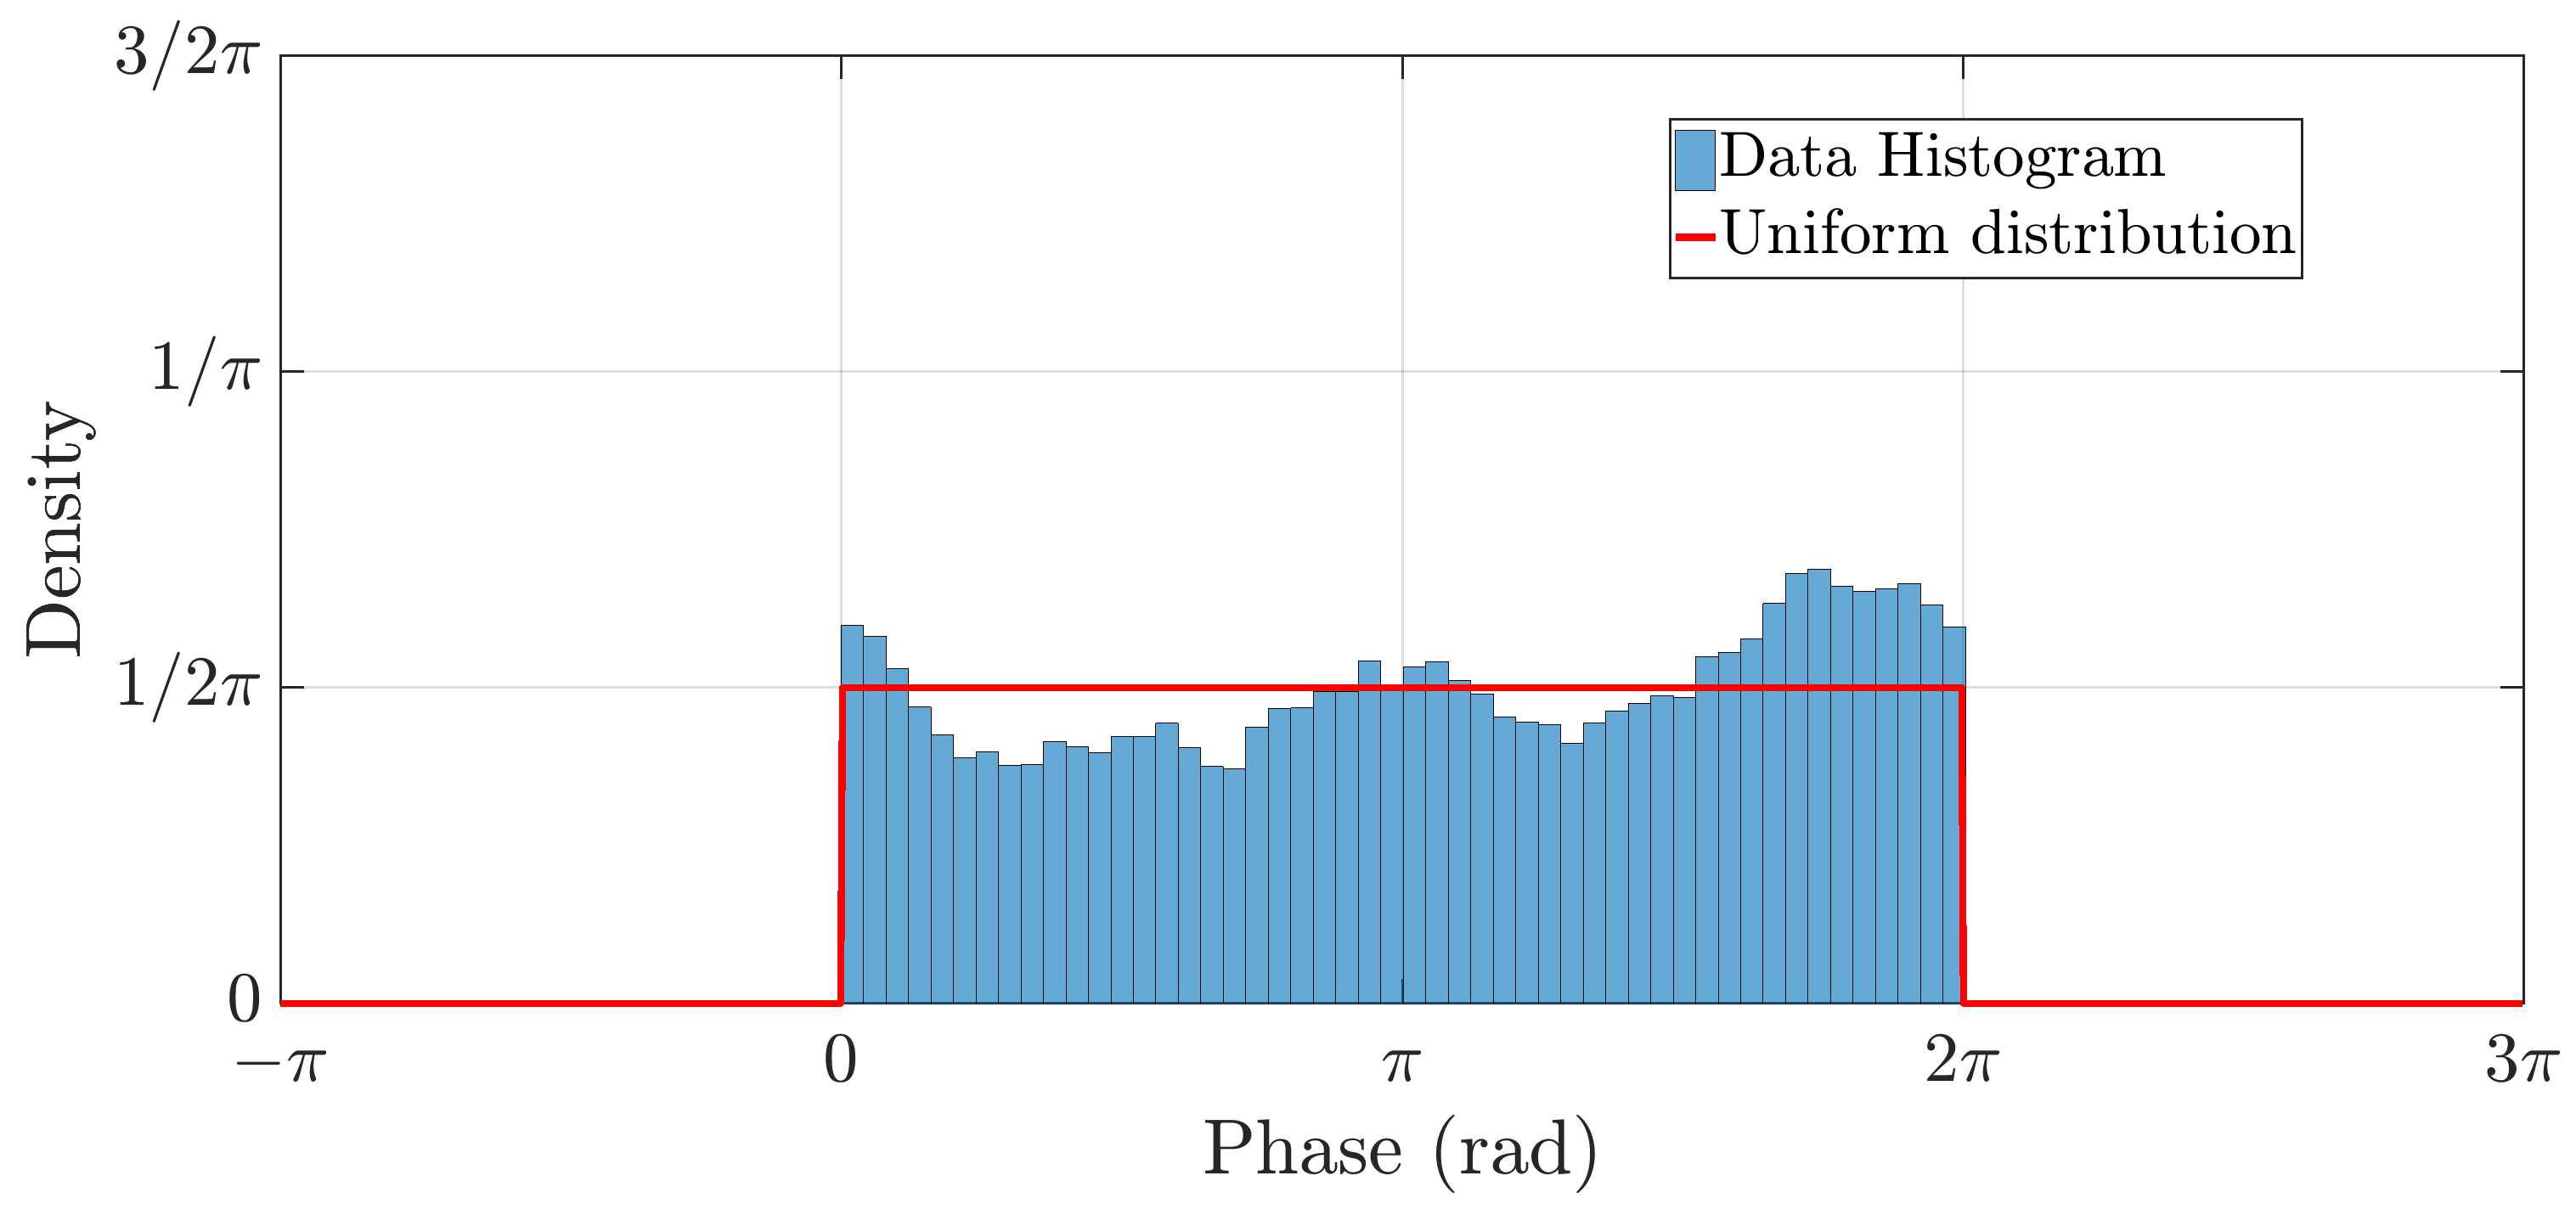
\includegraphics[width=0.9\textwidth]{images/Phase_histlW_2.eps}
	\caption{The relative frequency of the phase of the valid CFR estimates at the sample $k$ = 1060 ($k\Delta f= 51.76$ MHz) using the Uniform distribution.}
	\label{phase_examplelW}
\end{figure}

\begin{figure}[h!]
	\centering
	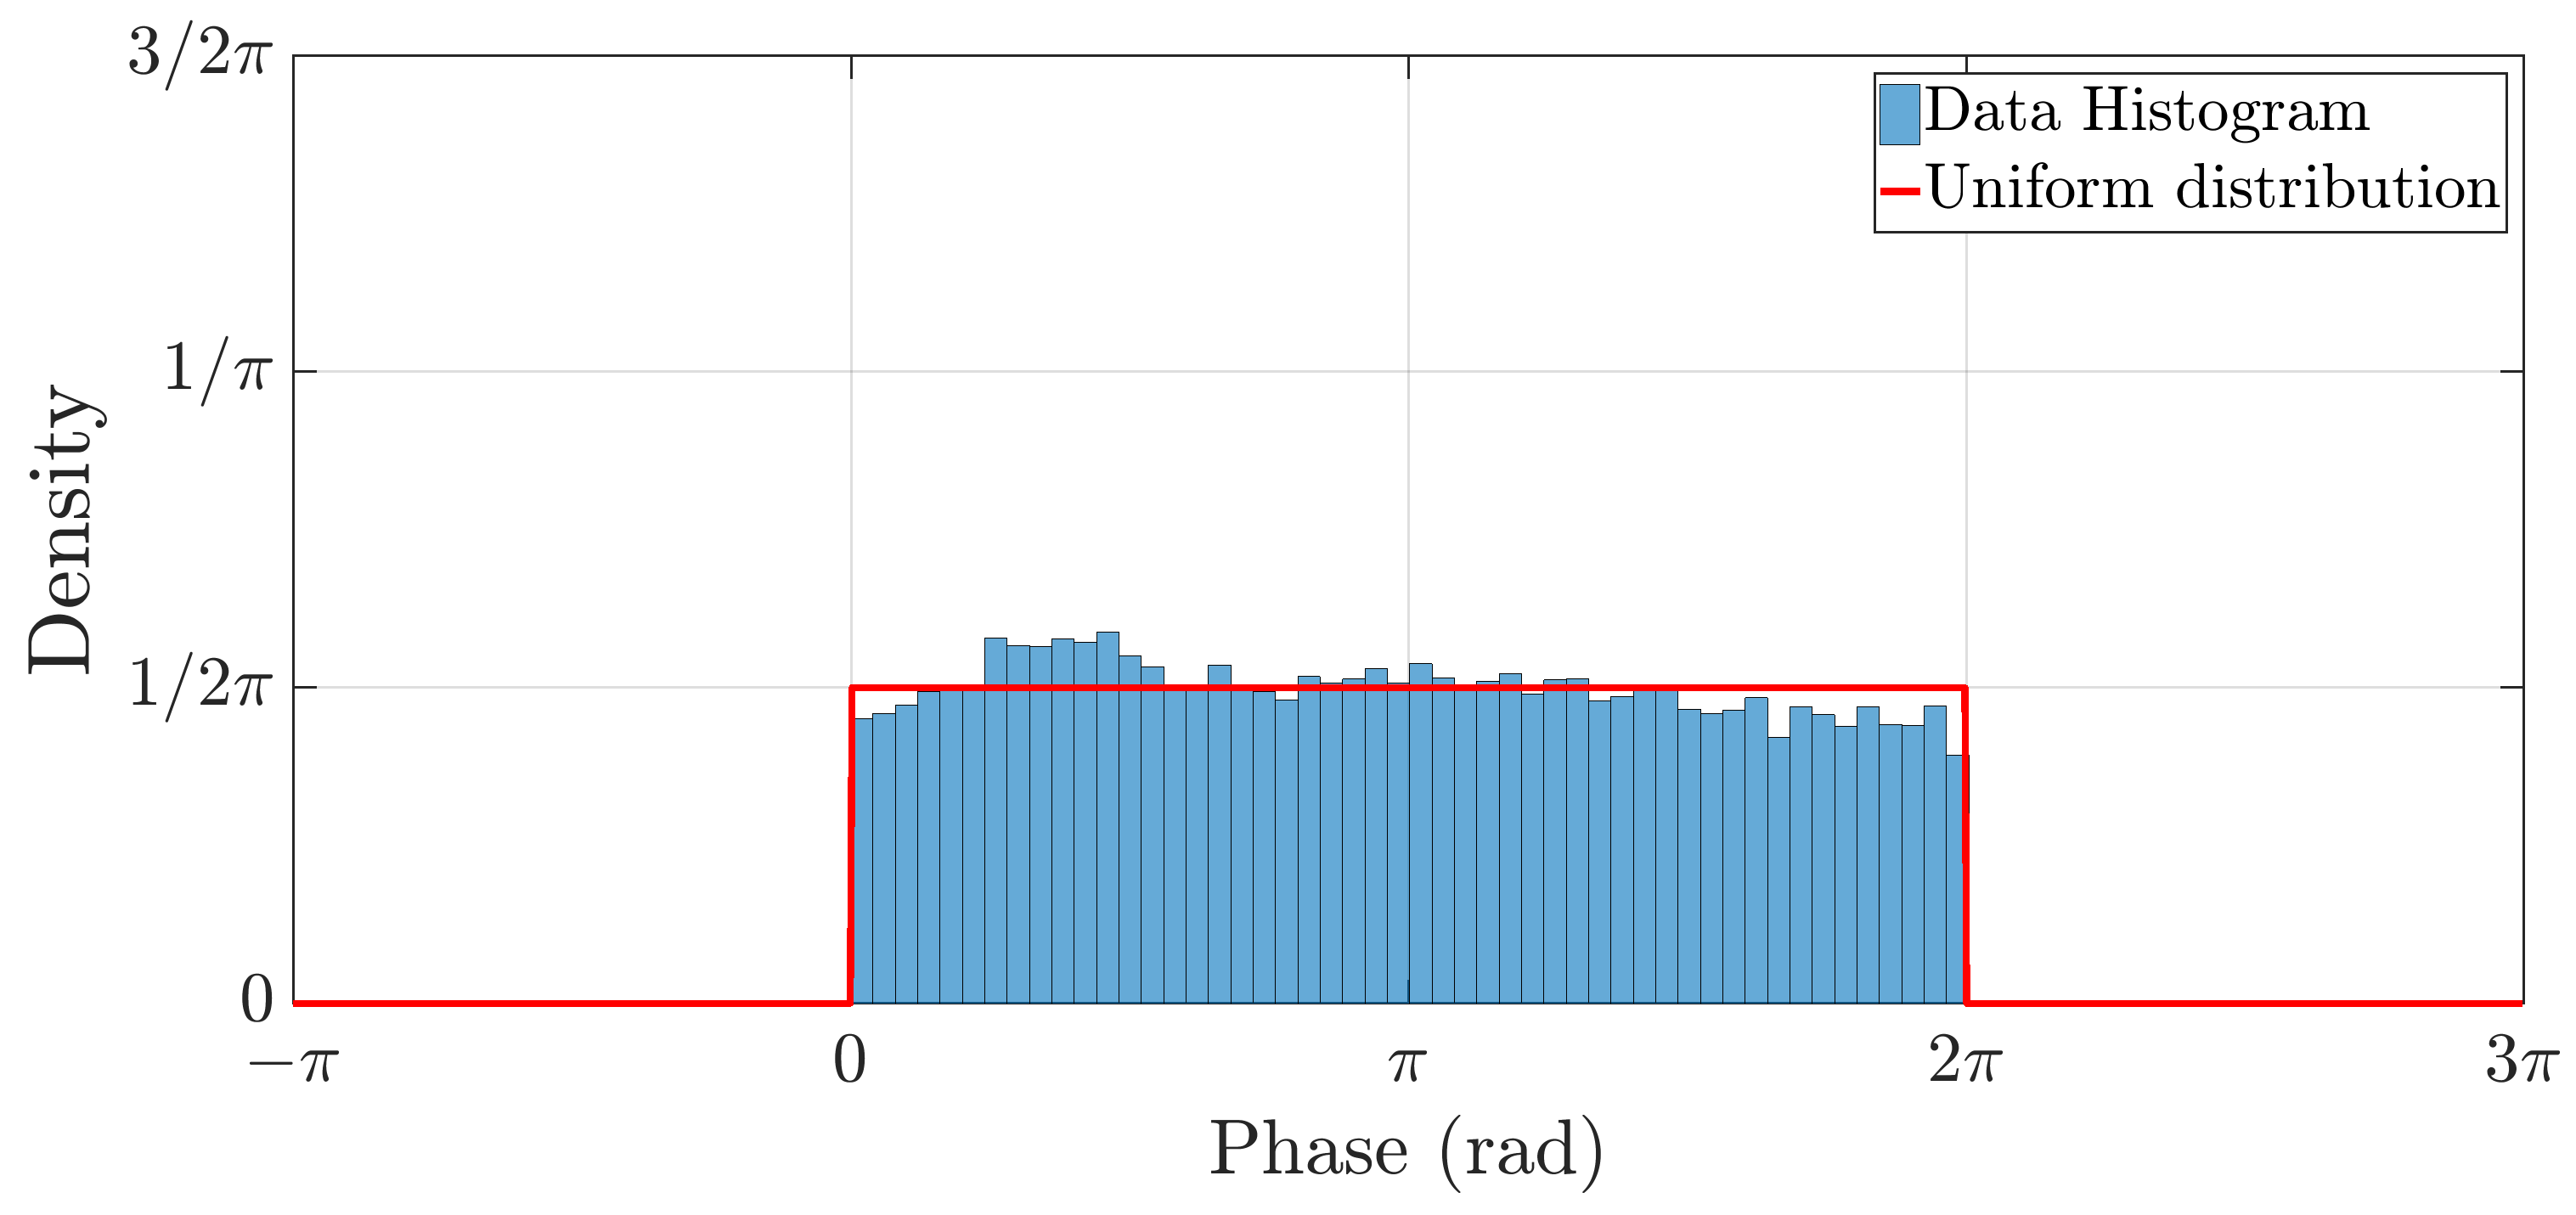
\includegraphics[width=0.9\textwidth]{images/Phase_hist2lW_2.eps}
	\caption{The relative frequency of the phase of the valid CFR estimates at the sample $k$ = 1600 ($k\Delta f= 78.1$ MHz) using the Uniform distribution.}
	\label{phase_example2lW}
\end{figure}

Overall, the use of the proposed enhanced statistical modeling method for modeling the \ac{CFR} of in-home \ac{PLC}-\ac{WLC} \textit{long-path} channels showed that the magnitude component of the in-home \ac{PLC}-\ac{WLC} \textit{long-path} channel can be modeled by the Log-normal distribution, with parameters value changing as the frequency varies, resulting in a non-stationary random process. The statistical analyses has also verified that the phase component of in-home \ac{PLC}-\ac{WLC} \textit{short-path} channels is a stationary random process, that can be modeled by the Uniform distribution.

%%%%%%%%%%%%%%%%%%%%%%%%%%%%%%%%%%%%%%%%%
\section{SUMMARY} \label{sec:NR5}
%%%%%%%%%%%%%%%%%%%%%%%%%%%%%%%%%%%%%%%%%

This chapter has presented statistical analyses of \acp{CFR} of \ac{PLC} and hybrid \ac{PLC}-\ac{WLC} channels, acquired through a measurement campaign. These analyses were performed by employing the enhanced statistical modeling method described in Chapter \ref{Proposal}. The statistical distributions offering the best models for the random processes ${|\bf{H}|}$ and ${\bf \Theta}$, which represent magnitude and phase components of the \ac{CFR}, respectively, were detailed for both \ac{PLC} and hybrid \ac{PLC}-\ac{WLC} scenarios in the frequency band from $1.7$ up to $100$~MHz.
